\setcounter{part}{21}   % M

\part{Mécanique} %1
\section{Oscillateur harmonique}
% Niveau :      PC
% Discipline :  Méca

\begin{exercise}{Questions préliminaires}{0}{Sup, Spé}
{Oscillateur harmonique,Questions préliminaires}{lelay}

Ces questions font appel soit directement au cours, soit à des raisonnements simples d'ordre de grandeur ou d'analyse dimensionnelle. Elles servent juste à aiguiser le sens physique : pas besoin de les rédiger. Il faut savoir y répondre rapidement.

\begin{questions}
    \question Donner la position à l'équilibre d'une masse $m$ attachée au plafond par un ressort de raiseur $k$. La pulsation des oscillations est-elle la même qui si le système était en position horizontale ?
    \question Donner la force minimale avec laquelle il faut appuyer sur une masse accrochée à un ressort contre un mur pour faire décoller le ressort du mur.
    \question Ordre de grandeur d'une raideur $k$ typique de ressort (ex : ressort de stylo à bille, ou stylo quatre couleurs).
    \question Quelles sont les approximations faites pour assimiler le système masse ressort à un oscillateur harmonique ?
\end{questions}
\end{exercise}
% Niveau :      PCSI 
% Discipline :  Méca

\begin{exercise}{\textit{L’amour est enfant de bohème}}{1}{Sup}
{Oscillateur harmonique}{strogatz}

Soit un couple canonique, Roméo et Juliette. On note $R$ l'affection que Roméo porte à Juliette et $J$ l'affection que Juliette porte à Roméo.

\newcommand{\heart}{\ensuremath\heartsuit}
\begin{questions}
    \question \textbf{The story of love and hate.} On considère que plus Roméo aime Juliette, plus celle-ci l'aime en retour. En revanche, plus Juliette s'attache à Roméo, moins il est attiré par elle. On modélise cette situation par
    \begin{align*}
        \dot J &= \alpha R, \\
        \dot R &= -\beta J,
    \end{align*} où $\alpha > 0$ et $\beta >0$.
    \begin{parts}
        \part Justifier le signe de $\alpha$ et $\beta$.
        \part Montrer que $R$ et $J$ vérifient chacun une équation d'oscillateur harmonique de pulsation $\omega_0$. Exprimer $\omega_0$ en fonction de $\alpha$ et $\beta$.
        \part En considérant la situation initiale $R(t=0) = R_0$ et $J(t=0)=0$, résoudre cette équation pour tout $t>0$.
        \part Montrer que la quantité
        $$\heart = \frac12 \alpha R^2+\frac12 \beta J^2$$
        est conservée. À quoi cette quantité vous fait-elle penser ?
        \part Portrait de phase : tracer la trajectoire du vecteur $(J(t), R(t))$ dans le plan $(J, R)$. Expliquer ce qu'il se passe. Donner une interprétation géométrique de $\heart$.
        \part Montrer que Roméo et Juliette ne sont jamais en phase pour le plus grand plaisir des dramaturges shakespeariens.
    \end{parts}
    \question \textbf{Roméo le robot.} On considère maintenant que Roméo aime tout le temps Juliette de la même manière : $\dot R = 0$.
    \begin{parts}
        \part Réécrire le système d'équation et le résoudre.
        \part Que se passe-t-il si $R(t=0) > 0$ ? Si $R(t=0) < 0$ ? 
        \part Celle fois-ci, {\heart} est-elle conservée ?
    \end{parts}
    \question \textbf{Juliette se méfie.} On considère maintenant que Juliette se méfie de cette relation : plus elle aime, plus elle doute. On modélise cela par $$\dot J = \alpha R - \gamma J,$$ avec $\gamma > 0$. 
    \begin{parts}
        \part Comment évolue $\heart$ avec le temps ? A priori, que vaut cette quantité lorsque $t \rightarrow \infty$ ?
        \part Écrivez l'équation vérifiée par $J(t)$, puis celle vérifiée par $R(t)$
        \part (\emph{Si vous avez fait les oscillateurs harmoniques amortis}) Résolvez cette équation et tracez la trajectoire de $(J,R)$ dans le portrait de phase.
    \end{parts}
\end{questions}

\vspace{15mm}

\begin{center}

\begin{minipage}{6cm}
    \itshape L'amour est enfant de bohème \\
    Il n'a jamais, jamais, connu de loi \\
    Si tu ne m'aimes pas, je t'aime \\
    Et si je t'aime, prends garde à toi
    
    \flushright Carmen, \normalfont Georges Bizet, 1875
\end{minipage}
\end{center}
\end{exercise}
% Niveau :      PCSI
% Discipline :  Méca


\begin{exercise}{Dynamique portuaire à Ploudalmézeau}{2}{Sup}
{Oscillateur harmonique}{lelay}

On considère le port breton de Ploudalmézeau dans le Finistère (29). Les principaux habitants en sont de fiers marins bretons, des goélands et des sardines dont les goélands sont friands.

On note $s(t)$ le nombre de sardines et $g(t)$ le nombre de goélands dans le port. Il y a en permanence de nouvelles sardines qui arrivent dans le port, attirées par le charme naturel des côtes bretonnes. De plus les goélands ont tendance à migrer vers l'intérieur des terres et à ne pas rester dans les environs du port. On modélise la situation comme suit :
\begin{align*}
    \dv{g}{t} &= b\:s(t) - \alpha \\
    \dv{s}{t} &= -c\:g(t) + \beta 
\end{align*}
\begin{questions}
    \question Justifier chacun des termes de la modélisation ci-dessus.
    \question Montrer que $g(t)$ et $s(t)$ obéissent chacun à une équation d'oscillateur harmonique de même pulsation.
    \question Trouver $g(t)$ et $s(t)$ sachant que à $t = 0$ jour, il y a 7 goélands et 250 sardines.
    \question Quel est le déphasage entre $g(t)$ et $s(t)$ ? Justifier qu'elles ne peuvent pas être en phase.
\end{questions}
\textbf{Données :} On pourra supposer que à l'équilibre la population de sardines est de 250 individus et celle de goélands de 5 individus, que chaque goéland mange 10 sardines par jour et qu'un nouveau goéland migre vers l'intérieur des terres chaque jour. 
\end{exercise}
% Niveau :      PCSI
% Discipline :  Méca

\begin{exercise}{Dynamique proie-prédateur}{3}{Sup}
{Oscillateur harmonique}{lelay}

L'exercise utilise un des modèles développés par Lotka et Volterra en 1925 pour modéliser les systèmes avec des proies et des prédateurs en interaction.

On considère une île au large de la Bretagne sur laquelle vivent des sardines et des goélands :
\begin{itemize}
    \item les sardines se reproduisent entre elles,
    \item les goélands se battent entre eux,
    \item les goélands mangent les sardines et se reproduisent si ils se sont suffisamment bien nourris.
\end{itemize}
On note $s(t)$ la population de sardines et $g(t)$ la population de goélands, et on considère la modélisation suivante :
\begin{align*}
    \dv{s}{t} &= a\:s(t) - b\:s(t)\:g(t) \\
    \dv{g}{t} &= -c\:g(t) + d\:s(t)\:g(t)
\end{align*}
\begin{questions}
    \question Justifier chacun des termes de la modélisation ci-dessus.
\uplevel{Faire un rictus de douleur à la vue de ce système d'équations, car il est non-linéaire : il n'a pas de solution analytique ! Mais cela ne nous empêchera pas de l'étudier.}
    \question Montrer que ce système admet deux \emph{points fixes}.\\
    Des points fixes sont des points d'équilibre $(s_0, g_0)$ tels que si pour un $t_0$ donné on a $s(t_0) = s_0$ et $g(t_0) = g_0$, alors $\forall t > t_0$, $s(t) = s_0$ et $g(t) = g_0$.
    \question On se place au voisinage du point fixe intéressant et on prend $s(t) = s_0 + x(t)$ et $g(t) = g_0 + y(t)$. Écrire les équations au premier ordre en $x$ et en $y$ (\emph{i.e.} les termes comme $x^2$, $y^2$ et $xy$ sont négligés devant les autres).
    \question Montrer qu'alors $x$ et $y$ obéissent à une équation d'oscillateur harmonique dont on exprimera la pulsation $\omega$ en fonction des paramètres du problème.
    \question Les sardines et les goélands peuvent-elles coexister ?
\end{questions}
\end{exercise}
% Niveau :      PCSI
% Discipline :  Méca

\begin{exercise}{Ressort sur un plan incliné}{1}{Sup}
{Mécanique,Oscillateur harmonique,Ressort}{lelay}

On considère une masse $m$ au bout d'un ressort sans masse de constante de raideur $k$ et de longueur à vide $\ell_0$ qui se déplace sans frottement sur un plan incliné d'un angle $\alpha$ par rapport à l'axe horizontal. Le ressort est fixé en $x=0$.

\begin{questions}
    \question Déterminer la longueur du ressort  à l'équilibre $\ell_\text{éq}$.
    \question On étire le ressort d'une longueur $\Delta\ell$, déterminer le mouvement du ressort. Commenter l'influence de l'angle pente ($\alpha$) sur les oscillations
    \question Retrouver ce résultat par des considérations énergétiques.
\end{questions}
\end{exercise}
% Niveau :      PCSI
% Discipline :  Méca

\begin{exercise}{Assemblage de ressorts}{1}{Sup}
{Mécanique,Oscillateur harmonique,Ressort}{lelay}

\begin{questions}
    \question Soit une masse reliée à un mur par deux ressorts de raideur $k_1$ et $k_2$, et de même longueur à vide $\ell_0$. Donner la raideur $k$ du ressort équivalent.
    \question Soit une masse reliée à un ressort de raideur $k_1$, lui même accroché à un ressort $k_2$ relié à un mur. Donner la raideur $k$ du ressort équivalent.
    \question Soit une masse reliée à un mur par deux ressorts de raideur $k_1$ et $k_2$, et de longueur à vide $\ell_1$ et $\ell_2$. Donner la distance de la masse au mur à l'équilibre en fonction des paramètres du problème.
    \question Soit une masse entre deux murs, reliée à chacun d'eux par un ressort de raideur $k$ et de longueur à vide $l_0$. Donner la position $x(t)$ de la masse en fonction du temps
    \questionbonus Quelle analogie peut-on faire avec l'assemblage de résistances en électronique ?
\end{questions}
\end{exercise}

% Niveau :      PCSI
% Discipline :  Méca

\begin{exercise}{Ressorts en chaîne}{2}{Sup}
{Mécanique,Oscillateur harmonique,Ressort}{lelay}

Dans cet exercice, tous les ressorts ont une raideur $k$ et une longueur à vide $a$, et toutes les masses ont une masse $m$.
\begin{questions}
    \question Soit une masse entre deux murs, reliée à chacun d'eux par un ressort. Donner la position $x(t)$ de la masse en fonction du temps
    \question Soit le système mur - ressort - masse - ressort - masse - ressort - mur. Donner les équations qui régissent le système.
    \begin{parts}
        \part Donner les équations qui régissent le système.
        \part En utilisant le changement de variable $X = x_1+x_2$ et $Y = x_1 - x_2$, résoudre le système et donner $X(t)$ et $Y(t)$
        \part En déduire $x_1(t)$ et $x_2(t)$. Interpréter.
    \end{parts}
    \question Soit le même système qui précédemment avec $N$ masses. Donner l'équation qui régit la masse $i$.
    \question On s'intéresse au cas $N=3$. % Ils sont en prépa faut bien qu'ils s'habituent à calculer un jour quand même.
    \begin{parts}
        \part Donner les équations qui régissent le système.
        \part En utilisant le changement de variable $X = x_1-x_3$, $Y = x_1 + \sqrt2 x_2 + x_3$ et $Z = x_1 - \sqrt2 x_2 + x_3$, résoudre le système et donner $X(t)$, $Y(t)$ et $Z(t)$
        \part Pensez-vous qu'il soit possible de généraliser ce processus ?
    \end{parts}
\end{questions}
\end{exercise}

% Niveau :      PCSI
% Discipline :  Méca

\begin{exercise}{Balle rebondissante}{2}{Sup}
{Mécanique, Oscillateur harmonique,Ressort}{lelay}

On considère une balle de masse $m$ qui se mouvoir verticalement dans le champ de gravité et sa hauteur par rapport au sol est notée $h$. En dessous de cette balle est accroché un ressort de raideur $k$ et de longueur $\ell_0$. Initialement, la balle est une la hauteur $h_0 > \ell_0$ du sol, et on la laisse tomber à $t = 0$. Attention, le ressort est fixé \textbf{uniquement} à la balle : en particulier, à $t=0$, il ne touche pas le sol.
\begin{questions}
    \questioncours Caractéristiques du mouvement de chute libre : trajectoire, évolution de la position et de la vitesse.
    \question Faire le bilan des forces sur la masse $m$ pour $h > \ell_0$.
    \question Donner les équations du mouvement et leur solution pour $h > \ell_0$
    \question  À quel temps $\tau_1$ la balle arrive-t-elle à une hauteur $\ell_0$ ? Que se passe-t-il alors ? 
    \question Faire le bilan des forces sur la masse $m$ pour $h \leq \ell_0$.
    \question En déduire les équations du mouvement. À quel temps $\tau_2$ la balle revient-elle à une hauteur $\ell_0$ ?
    \question Que se passe-t-il alors ? À quel temps $T$ la balle revient-elle à une hauteur $h_0$ ?
    \question Représenter graphiquement $h(t)$ en identifiant chaque phase du mouvement.
\end{questions}

\begin{solution}

\begin{questions}
    \questioncours Caractéristiques du mouvement de chute libre : trajectoire, évolution de la position et de la vitesse.
    \question C'est une chute libre. $F = -mg$, Le ressort ne touche pas le sol.
    \question $\ddot h = -g$, $\dot h  = -gt$, $h = h_0 - gt^2/2$
    \question À $\tau_1 = \sqrt{2(h_0 - \ell_0)/g}$ le ressort sous la balle touche le sol : le mouvement devient celui d'un système masse-ressort vertical.
    \question $F = -mg - k(h - \ell_0)$. deux forces.
    \question $\ddot h + \frac{k}m h= -g + \frac{k}m \ell_0$. La solution est 
    \begin{align*}
    h (t) &= A\cos(\omega_0t) + B \sin(\omega_0t) + \ell_0 - mg/k \\ 
    h (t) &= A'\cos(\omega_0(t - \tau_1)) + B' \sin(\omega_0(t - \tau_1)) + \ell_0 - mg/k
    \end{align*}
    Avec $\omega_0 = \sqrt{k/m}$. Peu importe le détail des constantes, dans tous les cas le temps mis pour revenir à $\ell_0$ est une période, donc $$\frac{\omega_0}{2\pi} = \frac{1}{2\pi}\sqrt{k/m} $$
    
    % Par ailleurs
    % \begin{align*}
    % h (\tau_1) = A' + \ell_0 - mg/k = \ell_0 \\
    % \dot h (\tau_1) = \omega_0 B' = - g\tau_1
    % \end{align*}
    % D'où $A' = mg/k$ et $B'= -g\tau_1 / \omega_0$
    
    D'où $\tau_2 = \tau_1 + \frac{1}{2\pi}\sqrt{k/m}$
    \question La balle refait une chute libre mais à l'envers, elle met donc encore $\tau_1$ à revenir à $h_0$ ?
    \question Portion de parabole décroissante, portion de sinus, portion de parabole, etc...
\end{questions}
\end{solution}

% VIEILLE VERSION
% On considère un ressort de raideur $k$ et de longueur à vide $\ell_0$ posé verticalement sur une table, sur lequel est posé une masse $m$.
% \begin{questions}
%     \question Déterminer la position d'équilibre notée $z_0$ de la masse $m$ sur l'axe vertical $O_z$ dirigé vers le haut.
%     \question On appuie sur la masse $m$ avec une force $F$ de manière à la déplacer à la position $z_1 < z_0$. Faire le bilan des forces sur la masse $m$ et sur la table.
%     \question À $t=0$, on arrête soudainement d'appuyer sur le système ($F= 0$, $z = z_1$, $\dot{z} = 0$). Appliquer le PFD à la masse $m$ et donner $z(t)$ pour $t>0$.
%     \question Donner la condition pour que le ressort décolle de la table.
%     \question En supposant cette condition vérifiée, trouver l'instant $t_0$ où le ressort décolle. En déduire la vitesse $\dot{z}_0$ de la masse quand elle décolle.
%     \question Donner $z(t)$ pour $t > t_0$. À quelle altitude considérer que le ressort touche de nouveau le sol ?
%     \question Tracer le graphe de $z(t)$ pour $t\in\mbb{R}$ et expliquer chaque étape.
% \end{questions}
\end{exercise}

% Niveau :      PCSI
% Discipline :  Méca

\begin{exercise}{La figure de Lissajous}{1}{Sup}
{Mécanique,Oscillateur harmonique,Pendule}{lelay}

Soit un mobile $M$ accroché à un mur par un ressort de raideur $k$ et de longueur à vide $\ell_0$. Le mobile est situé sur un rail et ne peux bouger que selon l'axe $Ox$.
\begin{questions}
    \question Appliquer le PFD à $M$. Donner l'expression générale de la trajectoire $x_M(t)$ de $M$.
    \uplevel{On considère maintenant un autre mobile de masse $m$ relié à $M$ par un ressort $k$, $\ell_0$ dans une direction orthogonale $Oy$. $M$ et $m$ sont reliés de telle manière que à tout moment $x_m(t) = x_M(t)$.}
    \question Faire un schéma. Appliquer le PFD à $m$. Donner l'expression générale de la trajectoire $y_m(t)$ de $m$.
    \question Donner l'expression générale de la position $(x_m(t), y_m(t))$ du mobile $m$. Dessiner la trajectoire de $m$ pour :
    \begin{parts}
        \part $\omega_1 = \omega_2$, $\varphi_1 = \varphi_2$
        \part $\omega_1 = \omega_2$, $\varphi_1 = \varphi_2+\frac\pi2$
        \part $\omega_1 = \omega_2$, $\varphi_1 = \varphi_2+\pi$
        \part $\omega_1 = \omega_2$, $\varphi_1 = \varphi_2+3\frac\pi2$
        \part $\omega_1 = 2\omega_2$, $\varphi_1 = \varphi_2+\frac\pi2$
        \part $\omega_1 = n\omega_2$, $\varphi_1 = \varphi_2+\frac\pi2$, $n\in\mbb{N}$
        \part Que pouvez-vous conjecturer si $\omega_1/\omega_2$ est une fraction rationnelle ? Irrationnelle ?
    \end{parts}
\end{questions}
\end{exercise}
\begin{exercise}{Le pendule de Lissajous}{2}{Sup}
{Mécanique,Oscillateur harmonique,Pendule}{lelay}

\begin{questions}
    \questioncours Rappeler l'équation qui régit les mouvements d'un pendule de masse $m$ accroché à une corde de longueur $\ell$ et la résoudre pour des petits angles.
    
    \uplevel{On considère une corde de longueur $2L$ accrochée en haut de deux poteaux écartés de $D < 2L$. Au point le plus bas de la corde est accroché un pendule de masse $m$ et de longueur $R$.}
    \question Faire un schéma, et expliquer pourquoi on peut considérer les mouvements dans le plan des poteaux et dans le plan non horizontal qui lui est orthogonal comme indépendants.

    \question En considérant des petits angles, résoudre l'équation dans le plan des deux poteaux puis dans le plan orthogonal.
    \question Dessiner la trajectoire du mobile dans le plan horizontal pour $\omega_1 = \omega_2$
    \question Expliquer à quoi ressemblera (grossièrement) la trajectoire si $\frac{\omega_1}{\omega_2}$ est une fraction rationnelle
    \question A votre avis, Que si passe-t-il si $\frac{\omega_1}{\omega_2} $ est irrationnelle ?
\end{questions}
\end{exercise}
\begin{exercise}{Le slinky au repos}{2}{Sup}
{Mécanique,Oscillateur harmonique,Ressort}{lelay}

À la fin de cet exercice, on aura modélisé la forme au repos d'un slinky (les grands ressorts qui descendent les escaliers tous seuls).
\begin{questions}
    \questioncours Force exercée par un ressort. Lois d'association de ressorts.
    \uplevel{On considère un assemblage constitué d'un mobile de masse $m_1$, reliée horizontalement à un mur situé en $x = 0$ par un ressort de raideur $k_1$ et de longueur à vide $\ell_1$. On repère la position de la masse par rapport au mur et on l'appelle $x(t)$.}
    \begin{center}
    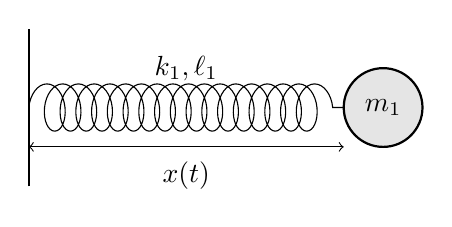
\begin{tikzpicture}
    
    \draw[thick, black] (0,-1) -- (0,1);
    
    \draw[decoration={aspect=0.6, segment length=2mm, amplitude=3mm,coil},decorate] (0,0) -- (4,0);
    \draw (2,0) node[above=6pt] {$k_1, \ell_1$};
    
    \filldraw[thick, color=black, fill=black!10] (4.5,0) circle (0.5);
    \draw (4.5,0) node {$m_1$};
    
    \draw[<->] (0,-0.5) -- (4,-0.5);
    \draw (2,-0.5) node[below=2pt] {$x(t)$};
    
    \end{tikzpicture}
    \end{center}
    \question Décrire qualitativement puis quantitativement les mouvements de perturbation d'amplitude initiale $y_0$ autour de la position de repos de la masse ? On appellera $y$ l'écart à l'équilibre.
    \question Comment évolue ce résultat si on suppose que le ressort est maintenant vertical et soumis à la gravité $g$ ?
    \uplevel{Cette fois-ci on utilise deux mobiles de masse $m_2$ et deux ressorts, de raideur $k_2$ et de longueur à vide $\ell_2$, comme dans l'illustration ci-dessous.}
    \begin{center}
    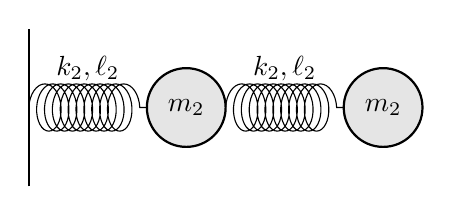
\begin{tikzpicture}
    
    \draw[thick, black] (0,-1) -- (0,1);
    
    \draw[decoration={aspect=0.6, segment length=1mm, amplitude=3mm,coil},decorate] (0,0) -- (1.5,0);
    \draw (0.75,0) node[above=6pt] {$k_2, \ell_2$};
    
    \filldraw[thick, color=black, fill=black!10] (2,0) circle (0.5);
    \draw (2,0) node {$m_2$};
    
    \draw[decoration={aspect=0.6, segment length=1mm, amplitude=3mm,coil},decorate] (2.5,0) -- (4,0);
    \draw (3.25,0) node[above=6pt] {$k_2, \ell_2$};
    
    
    \filldraw[thick, color=black, fill=black!10] (4.5,0) circle (0.5);
    \draw (4.5,0) node {$m_2$};
    
    \end{tikzpicture}
    \end{center}
    \question Que doivent valoir $m_2$ et $\ell_2$ pour que la position au repos de la masse la plus à droite et la masse totale soient les mêmes que précédemment ?
    \question On maintient la masse la plus à droite à une distance $y$ de sa position d'équilibre.
    \begin{parts}
        \part À l'équilibre, quelle est la position de la masse du milieu ? 
        \part Quelle est la force exercée par le ressort le plus à droite sur la masse la plus à droite ?
        \part Que doit valoir $k_2$ pour que cette force soit la même qu'avec l'assemblage précédent ?
    \end{parts}
    \question Comment choisir $\ell_n$, $m_n$ et $k_n$ dans le cas de $n$ masses ?
    
    \uplevel{On considère maintenant le même assemblage de deux masses $m_2$ que précédemment, mais cette fois à la verticale.}
    \question Quelle est la position d'équilibre de chaque ressort ?
    \question S'il y en a maintenant $n$, comment évolue l'écart entre chaque spire ?
\end{questions}
\end{exercise}


\section{Cinématique du point}
% % Niveau :      PC
% Discipline :  Méca

\begin{exercise}{Questions préliminaires}{0}{Sup, Spé}
{Cinématique, Questions préliminaires}{lelay}

Des petites questions pour commencer une colle dans la joie et la bonne humeur. Elles font appel soit directement au cours, soit à des raisonnements simples d'ordre de grandeur ou d'analyse dimensionnelle. Elles servent juste à aiguiser le sens physique : pas besoin de les rédiger. Il faut savoir y répondre rapidement.

\begin{questions}
    \question Donner la vitesse et l'accélération d'une particule en coordonnées sphériques et interpéter physiquement chaque terme.
\end{questions}
\end{exercise}
% \begin{exercise}{Questions de cinématique}{1}{Sup}
{Cinématique}{lelay}


\begin{questions}
    \questioncours Rappeler les caractéristiques des coordonnées cartésiennes, polaires et sphériques.
    \question Quel est le système de coordonnées le plus simple a priori ? Exprimez la position, la vitesse et l'accélération d'un point dans ce système de coordonnées.
    \question On s'intéresse dans un premier temps aux coordonnées polaires 
    \begin{parts}
        \part Montrez qu'on peut toujours trouver un repère cartésien $\ve_x, \ve_y, \ve_z$ tel que $\ve_r$ et $\ve_\theta$ peuvent s'exprimer seulement en fonction de $r, \theta, \ve_x$ et $\ve_y$
        \part Quelle est alors l'expression du vecteur position $\vec{OM}$ en coordonnées cylindriques ?
        \part Montrez qu'on a $\dv{\ve_r}{t} = \ve_\theta$. Comment interpréter cela graphiquement ? En déduire $\dv{\ve_\theta}{t}$.
        \part Démontrez la formule de la vitesse en cylindrique
        \part Démontrez la formule de l'accélération en cylindrique
    \end{parts}
    \question On s'intéresse ensuite aux coordonnées sphérique 
    \begin{parts}
        \part Le problème de la conversion cartésien -- sphérique peut-il toujours se ramener à un problème plan ?
        \part Quelle est l'expression du vecteur $\vec{OM}$ en coordonnées sphériques ?
        \part Montrez que le volume élémentaire en sphérique est donnée par $\dd{\tau} = \dd{r} \times r \dd{\theta} \times r \sin\theta \dd{\varphi}$
        \part Démontrez la formule de la vitesse en sphérique
        \part Démontrez la formule de l'accélération en sphérique
    \end{parts}
\end{questions}

\end{exercise}

\begin{solution}
J'avoue que l'accélération en sphérique je la sais pas par coeur lol
\end{solution}

\begin{exercise}{Mouvement d'un satellite}{1}{Sup}
{Cinématique}{lelay}

On considère un satellite en mouvement circulaire uniforme au dessus de la Terre. Il ressent une accélération 
$$a = g \qty(\dfrac{R}{r})^2,$$
avec $R$ le rayon de la Terre et $r$ le rayon de l'orbite. Ce satellite est dit géostationnaire, c'est-à-dire que la période de révolution du satellite est égale à la période de rotation propre de la Terre.


\begin{questions}
    \questioncours Rappeler les caractéristiques (position, vitesse, accélération) du mouvement circulaire uniforme. Qu'est-ce qui change si le mouvement n'est plus uniforme ?
    
    \question Déterminer l'altitude du satellite.
    
    \question Calculer la norme de la vitesse du satellite.
    
    \question Quel est, selon vous, l'intérêt d'un tel satellite ? Les inconvénients ?
\end{questions}

\end{exercise}

\begin{solution}

\begin{questions}
    \questioncours Rappeler les caractéristiques (position, vitesse, accélération) du mouvement circulaire uniforme. Qu'est-ce qui change si le mouvement n'est plus uniforme ?
    
    \question $a = r\omega^2$, 36 000 km (42 000 avec le rayon de la Terre)
    
    \question $v = a\omega$
    
    \question Intéret : ca bouge pas donc ca couvre la moitie de la surface de la Terre en continu. Inconvenient : aux bords de la zone couverte ça recoit mal. Or geostationnaire ce n'est possible qu'au dessus de l'équateur, donc les pôles l'ont dans l'os. 
    
    On utilise alors des orbites géosynchrones, qui ont une certaine inclinaison. Pb : La moitié du temps on couvre un pole, l'autre moitié l'autre (alors qu'on s'en fout).
    
    Solution : On utilise des orbites excentriques pour passer la plupart du temps dans la zone intéressante. Voir par ex l'orbite de Molnya (période 12h).
\end{questions}

\end{solution}

\begin{exercise}{Mouvement sur une ellipse}{1}{Sup}
{Cinématique}{lelay}

On considère un mobile $M$ se déplaçant sur une ellipse de demi grand axe $a$ et de demi petit axe $b$ en suivant les équations horaires suivantes
\begin{align*}
    \left\{
    \begin{array}{ccc}
         x(t) &=& \alpha \cos(\omega t + \phi) \\
         y(t) &=& \beta \sin(\omega t + \psi)
    \end{array}
    \right.
\end{align*}

\begin{center}
    \begin{tikzpicture}
    
    % x
    \draw[gray, thick, ->] (-5,0) -- (6,0);
    \draw (6,0) node[below=2pt] {$x$};
    
    % y
    \draw[gray, thick, ->] (0,-2.5) -- (0,3);
    \draw (0,3) node[left=2pt] {$y$};
    
    % centre, ellipse
    \node (C) at (0,0) {};
    \draw (0,0) ellipse (4 and 2);
    \path (C) -- coordinate[midway](A) (3,0);
    \draw (A) node[below=2pt] {$a$};
    \path (C) -- coordinate[midway](B) (0,2);
    \draw (B) node[left=2pt] {$b$};
    
    % Point
    \node (L) at (4,0) {};
    \filldraw[black,thick] (L) circle [radius=3pt] ;
    \draw (L) node[above right=2pt] {$L$};
    
    % Point quelconque
    \node (M) at (1.41*2,1.41) {};
    \filldraw[black,thick] (M) circle [radius=3pt] ;
    \draw (M) node[above right=2pt] {$M$};
    
    \draw[gray, thick, dotted] (C) -- (M);
    \draw[black] (2,0) arc (0:25:2);
    \draw (1.41,0.707) node[below right=2pt] {$\theta$};
    
    \end{tikzpicture}
\end{center}

\begin{questions}
    \questioncours Définir les coordonnées polaires et donner la correspondance entre ce système de coordonnées et le système cartésien.
    \question On indique qu'à $t = 0$, le mobile est situé sur le point $L$. En déduire les valeurs de $\alpha$, $\phi$ et $\psi$
    \question Des autres données, déduire la valeur du coefficient $\beta$
    \question Déterminer les composantes de la vitesse $(\dot x , \dot y)$ et de l'accélération $(\ddot x, \ddot y)$
    \question Montrez que l'accélération est de la forme $\vec{a} = - K \vec{OM}$. Déterminer la valeur de la constante $K$.
    \question Donner les équations horaires du mouvement en utilisant les coordonnées polaires.
    \question Que donnent les expressions précédentes pour $b = a$ ?
\end{questions}

\end{exercise}

\begin{solution}

\begin{questions}
    \questioncours Définir les coordonnées polaires et donner la correspondance entre ce système de coordonnées et le système cartésien.
    \question $\alpha = a$, $\phi = 0$, $\psi = 0$
    \question $\beta = b$
    \question Calcul de dérivées par rapport au temps
    \question $K = \omega^2$. Remarque sur l'analyse dimensionnelle.
    \question $r = \sqrt{x^2 + y^2}$, $\tan\theta = \frac{b}a \tan\omega t$
    \question Cercle, $r=r_0$ $\dot\theta = \omega$
\end{questions}

\end{solution}

\begin{exercise}{La torpille}{1}{Sup}
{Cinématique}{lelay}

Un navire $N$ est animé d'un mouvement rectiligne uniforme de vitesse $\vec{v}$ le long d'une droite $D$. Un sous marin immobile $S$ tire une torpille $T$ de vitesse $\vec{u}$ au moment à l'angle $(\vec{SN}, \vec{v})$ vaut $\alpha$.

\begin{center}
    \begin{tikzpicture}
    
    % Le navire
    \node (N) at (-4,0) {};
    \filldraw[black,thick] (N) circle [radius=3pt] ;
    \draw (N) node[above=2pt] {$N$};
    
    % La trajectoire
    \draw[gray, thick] (-5,0) -- (2,0);
    \draw (1.5,0) node[above=1pt] {$D$};
    
    % Le vecteur vitesse
    \node (v) at (-2,0) {};
    \draw[black, thick, ->] (N) -- (v);
    \path (N) -- coordinate[midway](labelv) (v);
    \draw (labelv) node[above=2pt] {$\vec{v}$};
    
    % Le sous marin
    \node (S) at (0,-3) {};
    \filldraw[black,thick] (S) circle [radius=3pt] ;
    \draw (S) node[below=2pt] {$S$};
    
    % La droite
    \draw[gray, thick, dotted] (S) -- (N);
    \draw[black] (-2.5,0) arc (0:-36.9:1.5);
    \draw (-2.5,-0.5) node[anchor=west] {$\alpha$};
    
    % Interception des trajectoires (cible)
    \node (C) at (-1,0) {};
    % \filldraw[black,thick] (C) circle [radius=3pt] ;
    % \draw (C) node[above=2pt] {$C$};
    
    % Trajectoire de la torpille
    \draw[gray, thick, dotted] (S) -- (C);
    
    % Position de la torpille
    \path (S) -- coordinate[midway](T) (C);
    \filldraw[black,thick] (T) circle [radius=2pt] ;
    \draw (T) node[right=2pt] {$T$};
    
    % Vecter vitesse de la torpille
    \path (T) -- coordinate[midway](u) (C);
    \draw[black, thick, ->] (T) -- (u);
    \path (T) -- coordinate[midway](labelu) (u);
    \draw (labelu) node[above right=1.5pt] {$\vec{u}$};
    
    \draw[black] (T) arc (105:143:1.5);
    \draw (-1.4,-1.5) node[anchor=west] {$\theta$};
    
    
    \end{tikzpicture}
\end{center}

\begin{questions}
    \questioncours Rappeler la définition d'un référentiel et d'un repère. Dans quel référentiel se place-t-on ici ?
    \question Commenter le schéma et identifier les cas limites.
    \question Quelle doit être la valeur de l'angle de tir $\theta = (\vec{SN}, \vec{u})$ pour que la torpille atteigne sa cible ?
    \question On souhaite que la torpille atteigne le navire en un temps minimum. Pour quelle valeur de $\alpha$ convient-il de tirer ? Calculer l'angle de tir correspondant. Interpréter ces résultats dans les limites $ u \gg v$ et $u \ll v$
\end{questions}

\end{exercise}

\begin{solution}


\begin{questions}
    \questioncours Rappeler la définition d'un référentiel et d'un repère. Dans quel référentiel se place-t-on ici ?
    \question L'idée est de réfléchir physiquement. Plein de choses à dire en regardant le dessin, par exemple :
    \begin{itemize}
        \item $u \gg v$ : $\theta \rightarrow 0$
        \item $v \gg u$ : impossible
        \item Si $\alpha \geq \pi/2$, on doit avoir $u \geq v$
        \item Si $\alpha = \pi/2$ et $u = v$, $\theta = \pi/4$
    \end{itemize}
    
    \question 2 possibilités :
    \begin{itemize}
        \item Utiliser la distance MC, M étant le projeté orthogonal du point de croisement des trajectoires (C) sur la droite reliant S à N. la distance MC est alros $MC = d = ut \sin \theta = v t \sin \alpha$ avec $t$ le temps de trajet de la torpille
        \item Partir directement de la loi des sinus : $\sin \alpha / uT = \sin \theta / vT$
    \end{itemize}
    À la fin on doit trouver $u \sin \theta = v \sin \alpha$
    
\begin{center}
    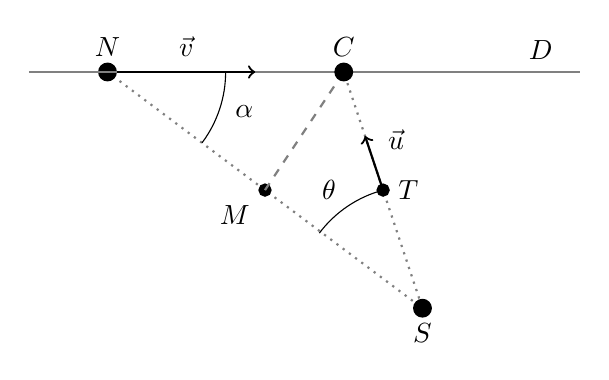
\begin{tikzpicture}
    
    % Le navire
    \node (N) at (-4,0) {};
    \filldraw[black,thick] (N) circle [radius=3pt] ;
    \draw (N) node[above=2pt] {$N$};
    
    % La trajectoire
    \draw[gray, thick] (-5,0) -- (2,0);
    \draw (1.5,0) node[above=1pt] {$D$};
    
    % Le vecteur vitesse
    \node (v) at (-2,0) {};
    \draw[black, thick, ->] (N) -- (v);
    \path (N) -- coordinate[midway](labelv) (v);
    \draw (labelv) node[above=2pt] {$\vec{v}$};
    
    % Le sous marin
    \node (S) at (0,-3) {};
    \filldraw[black,thick] (S) circle [radius=3pt] ;
    \draw (S) node[below=2pt] {$S$};
    
    % La droite
    \draw[gray, thick, dotted] (S) -- (N);
    \draw[black] (-2.5,0) arc (0:-36.9:1.5);
    \draw (-2.5,-0.5) node[anchor=west] {$\alpha$};
    
    % Interception des trajectoires (cible)
    \node (C) at (-1,0) {};
    \filldraw[black,thick] (C) circle [radius=3pt] ;
    \draw (C) node[above=2pt] {$C$};
    
    % Trajectoire de la torpille
    \draw[gray, thick, dotted] (S) -- (C);
    
    % Position de la torpille
    \path (S) -- coordinate[midway](T) (C);
    \filldraw[black,thick] (T) circle [radius=2pt] ;
    \draw (T) node[right=2pt] {$T$};
    
    % Vecter vitesse de la torpille
    \path (T) -- coordinate[midway](u) (C);
    \draw[black, thick, ->] (T) -- (u);
    \path (T) -- coordinate[midway](labelu) (u);
    \draw (labelu) node[above right=1.5pt] {$\vec{u}$};
    
    % angle theta
    \draw[black] (T) arc (105:143:1.5);
    \draw (-1.4,-1.5) node[anchor=west] {$\theta$};
    
    % Projeté orthogonal
    \path (N) -- coordinate[midway](M) (S);
    \filldraw[black,thick] (M) circle [radius=2pt] ;
    \draw (M) node[below left=2pt] {$M$};
    
    \draw[gray, thick, dashed] (M) -- (C);
    
    \end{tikzpicture}
\end{center}
    
    \question Il faut que la trejectoire de la torpille soit minimale : On frappe le navire lorsque il est a la distance minimale. On a alors $\theta = \arctan v/ u$ et $\alpha = \arctan(u / v)$
    
\begin{center}
    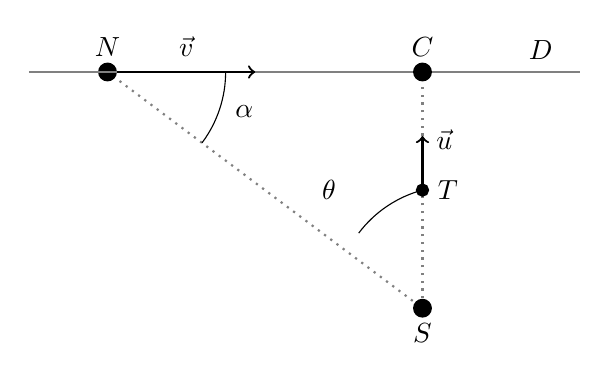
\begin{tikzpicture}
    
    % Le navire
    \node (N) at (-4,0) {};
    \filldraw[black,thick] (N) circle [radius=3pt] ;
    \draw (N) node[above=2pt] {$N$};
    
    % La trajectoire
    \draw[gray, thick] (-5,0) -- (2,0);
    \draw (1.5,0) node[above=1pt] {$D$};
    
    % Le vecteur vitesse
    \node (v) at (-2,0) {};
    \draw[black, thick, ->] (N) -- (v);
    \path (N) -- coordinate[midway](labelv) (v);
    \draw (labelv) node[above=2pt] {$\vec{v}$};
    
    % Le sous marin
    \node (S) at (0,-3) {};
    \filldraw[black,thick] (S) circle [radius=3pt] ;
    \draw (S) node[below=2pt] {$S$};
    
    % La droite
    \draw[gray, thick, dotted] (S) -- (N);
    \draw[black] (-2.5,0) arc (0:-36.9:1.5);
    \draw (-2.5,-0.5) node[anchor=west] {$\alpha$};
    
    % Interception des trajectoires (cible)
    \node (C) at (0,0) {};
    \filldraw[black,thick] (C) circle [radius=3pt] ;
    \draw (C) node[above=2pt] {$C$};
    
    % Trajectoire de la torpille
    \draw[gray, thick, dotted] (S) -- (C);
    
    % Position de la torpille
    \path (S) -- coordinate[midway](T) (C);
    \filldraw[black,thick] (T) circle [radius=2pt] ;
    \draw (T) node[right=2pt] {$T$};
    
    % Vecter vitesse de la torpille
    \path (T) -- coordinate[midway](u) (C);
    \draw[black, thick, ->] (T) -- (u);
    \path (T) -- coordinate[midway](labelu) (u);
    \draw (labelu) node[above right=1.5pt] {$\vec{u}$};
    
    % angle theta
    \draw[black] (T) arc (105:143:1.5);
    \draw (-1.4,-1.5) node[anchor=west] {$\theta$};
    
    
    \end{tikzpicture}
\end{center}
\end{questions}

\end{solution}

\begin{exercise}{Les quatres chiens}{2}{Sup}
{Cinématique}{lelay}

À l'instant $t = 0$, quatre chiens $A$, $B$, $C$ et $D$ initialement situés aux sommets d'un carré de côté $\ell_0$ se mettent en mouvement l'un vers l'autre. $A$ se dirige vers $B$ qui se dirige vers $C$ qui se dirige vers $D$ qui lui-même se dirige vers $A$. Tous les chiens se déplacent à la même vitesse $V$.
\begin{questions}
    \questioncours Donner la définition d'un repère et d'un système de coordonnées. Citer ceux que vous connaissez en expliquant leur fonctionnement.
    \question Faire un schéma. Représenter les positions des chiens ainsi que leurs vecteurs vitesse à $t = 0$, pour $t > 0$ et pour $t = \infty$.
    \question Argumenter que le quadrilatère $ABCD$ reste carré, de côté $\ell(t)$ (on pourra invoquer les symétries de la situation). $\ell(t)$ est-elle une fonction croissante ou décroissante du temps ?
    \question Montrer que $\dv{\ell}{t} = - v$. 
    \question En déduire la durée $t_f$ de la poursuite.
    \question Quelle est la distance $D$ parcourue par chaque chien ?
    \question Déterminer, en coordonnées polaires, l'équation horaire de la trajectoire d'un chien dans un repère à l'origine bien choisie.
\end{questions}

\end{exercise}

\begin{solution}
\begin{questions}
    \questioncours Donner la définition d'un repère et d'un système de coordonnées. Citer ceux que vous connaissez en expliquant leur fonctionnement.
    \question Sa toune
    \question Symétrie SO4, $\ell$ diminue.
    \question Y a plein de manières, On peut écrire $\ell^2 = (\vec{OB} - \vec{OA})^2$, et dériver. 
    \question On a $\dot \ell = - v$ d'où $t_f = \ell_0 / v$, 
    \question Les chiens se déplacent à la vitesse $v$, donc $D = v t_f = \ell_0$
    \question On met le centre au centre. On écrit le vecteur déplacement $\vec{\dd{\ell}}$ de norme $v \dd{t}$ que l'on décompose en deux composantes ($\dd{r}$ sur $\vec{e_r}$ et $r\dd{\theta}$ sur $e_\theta$), d'où $\dot r = \cos \pi/4 v$ et $r\dot\theta = \cos \pi/4 v$ et donc $r(t) = \ell_0 - \frac{\sqrt{2}}{2} vt$ et $\theta(t) =  \int_0^t \frac{\sqrt{2}v}{2r(t)}\dd{t}$
\end{questions}



$t_f = 2/3 \ell_0 / v$, $D = 2 / 3 \ell_0$, en polaire $r = r_0 - \sqrt{3}/2 v t$ et $\theta = V/(2r)$
\end{solution}
,
\begin{exercise}{Les trois chiens}{3}{Sup}
{Cinématique}{lelay}

À l'instant $t = 0$, trois chiens $A$, $B$ et $C$ initialement situés aux trois sommets d'un triangle équilatéral de côté $\ell_0$ se mettent en mouvement l'un vers l'autre. $A$ se dirige vers $B$ qui se dirige vers $C$ qui lui-même se dirige vers $A$. Les trois chiens se déplacent à la même vitesse $v$.
\begin{questions}
    \questioncours Donner la définition d'un repère et d'un système de coordonnées. Citer ceux que vous connaissez en expliquant leur fonctionnement.
    \question Faire un schéma. Représenter les positions des trois chiens ainsi que leurs vecteurs vitesse à $t = 0$, pour $t > 0$ et pour $t = \infty$.
    \question Argumenter que le triangle $ABC$ reste équilatéral, de côté $\ell(t)$ (on pourra invoquer les symétries de la situation). $\ell(t)$ est-elle une fonction croissante ou décroissante du temps ?
    \question Montrer que $\dv{\ell}{t} = \dfrac{\vec{v_A} \vdot \vec{v_B}}{v} - v$. 
    \question En déduire la durée $t_f$ de la poursuite.
    \question Quelle est la distance $D$ parcourue par chaque chien ?
    \question Déterminer, en coordonnées polaires, l'équation horaire de la trajectoire d'un chien dans un repère à l'origine bien choisie.
    \questionbonus Comment généraliser ceci à $N$ chiens ?
\end{questions}

\end{exercise}

\begin{solution}
\begin{questions}
    \questioncours Donner la définition d'un repère et d'un système de coordonnées. Citer ceux que vous connaissez en expliquant leur fonctionnement.
    \question Sa toune
    \question Symétrie SO3, $\ell$ diminue.
    \question Y a plein de manières, On peut écrire $\ell^2 = (\vec{OB} - \vec{OA})^2$, et dériver. 
    \question On a $\dot \ell = -3/2 v$ d'où $t_f = 2/3 \ell_0 / v$, 
    \question Les chiens se déplacent à la vitesse $v$, donc $D = v t_f = 2 / 3 \ell_0$
    \question On met le centre au centre. On écrit le vecteur déplacement $\vec{\dd{\ell}}$ de norme $v \dd{t}$ que l'on décompose en deux composantes ($\dd{r}$ sur $\vec{e_r}$ et $r\dd{\theta}$ sur $e_\theta$), d'où $\dot r = \cos \pi/6 v$ et $r\dot\theta = \cos \pi/3 v$ et donc $r(t) = \ell_0 - \frac{\sqrt{3}}{2} vt$ et $\theta(t) =  \int_0^t \frac{v}{2r(t)}\dd{t}$
\end{questions}



$t_f = 2/3 \ell_0 / v$, $D = 2 / 3 \ell_0$, en polaire $r = r_0 - \sqrt{3}/2 v t$ et $\theta = V/(2r)$
\end{solution}
,
\begin{exercise}{La tractrice}{3}{Sup}
{Cinématique}{lelay}

Claude Perrault (architecte français du XVIIe siècle) pose sa montre sur la table. Il la tient par le bout d'une chaînette de longueur $a$. Il avance alors sa main à une vitesse $v$ dans la direction orthogonale à la position initiale de la montre (à l'origine, la montre est en $(0,a)$ et le doigt de Charles est à tout instant $t$ à la position $(vt, 0)$). On dénote par $(x(t), y(t))$ la position de la montre.
\begin{questions}
    \question Faire un schéma. Que vaut $y(t)$ lorsque $t$ tend vers l'infini ? Même question pour $vt-x$.
    \question La distance entre la montre et le doigt est constante (c'est la longueur $a$ de la chaînette). Ecrire l'équation mathématique qui en découle.
    
    \question Dériver l'équation précédente par le temps pour obtenir la relation (1) :
    $$ y\dot y  + (x-vt)(\dot x - v) = 0$$
    
    \question Le vecteur vitesse de la montre est à tout instant dirigé de la montre vers le doigt. En déduire la relation (2) :
    $$ \dot y (x- vt) + \dot x y = 0$$
    
    \question En combinant les deux équations précédentes, obtenir la relation (3) :
    $$ \dot x = \frac{v}{a^2}(x-vt)^2$$
    \question Vérifier que la fonction $x_0(t) = vt-a$ est solution de (3). Quelle situation cela représente-t-il ?
    \question On va chercher une solution générale en s'aidant de la solution particulière. On utilisant la fonction $z$ telle que $x(t) = x_0(t) + \frac1{z(t)}$, Montrer que $z$ vérifie l'équation différentielle (4) :
    $$
    \dot z = \frac{2v}{a}z - \frac{v}{a^2}
    $$
    \question Montrer que $z(t) = Ae^{2vt/a} + \frac{1}{2a}$, où $A$ est une constante dépendant des conditions initiales,
    est solution  de (4). On admettra que toutes les solutions de (4) peuvent se mettre sous cette forme.
    \question En déduire $x(t)$ et $y(t)$.
\end{questions}
La courbe qui décrit la trajectoire de la montre s'appelle la tractrice. Elle fait partie avec ses consoeurs la chaînette et la brachistochrone des grandes questions mathématiques des XVII et XVIII e siècle qui ont été résolues avec l'émergence du calcul différentiel.

\end{exercise}

\begin{solution}

\begin{questions}
    \question vers l'infini, $y\rightarrow 0$ et $vt-x \rightarrow a$
    \question $a^2 = y^2 + (x - vt)^2$
    \question Dériver l'équation précédente par le temps pour obtenir la relation (1) :
    $$ y\dot y  + (x-vt)(\dot x - v) = 0$$
    
    \question Le vecteur vitesse $\mqty( \dot x \\ \dot y)$ est colinéaire à $\mqty(vt - x, y)$. On peut donc faire le produit vectoriel entre les 2 pour obtenir 0 
    
    \question On peut par ex écrire $y (2)$, remplacer $y \dot y$ en utilisant (1) et $y^2$ par $a^2 - (x - vt)^2$ pour obtenir le résultat
    
    \question C'est la situation ou la chainette est initialement alignée avec le doigt
    
    \question Il faut écrire $\dot x$ de deux manières et les égaler.
    
    \question (4) étant une equadiff d'ordre 1, tout va bien
    
    \question En déduire $x(t)$ et $y(t)$.
\end{questions}
\end{solution}
\begin{exercise}{Brèves}{1}{Sup}
{Cinématique}{bermu}

Brèves de cinématique. On pourra prendre et justifier les approximations effectuées.

\begin{questions}
    \question Un skieur de 70 kg allant à 8.2 m$\cdot$s$^{-1}$ sur une piste verglacée tombe sur son dos (dans la même direction où il allait avant de tomber). 3 secondes après sa chute, sa vitesse est passée à 3.1 m$\cdot$s$^{-1}$.

    Quand le skieur s'arrète-t-il ? Quel distance aura-t-il parcouru durant sa chute ?

    \question Un couple de patineurs est initialement immobile sur la glace. Se repoussant avec leurs mains, la première personne, qui pèse 68 kg, communique à son ou sa partenaire, qui pèse 52 kg, une vitesse de 10 km/h sur la glace.
    
    Quelle est la vitesse finale des deux patineurs ?
\end{questions}

\end{exercise}

\begin{solution}

\end{solution}

% \begin{exercise}{La poursuite}{4}{Sup}
{Cinématique}{lelay}

On considère un étang circulaire de rayon $a$. A la circonférence de celui-ci se trouve un têtard, et au centre un poisson. À $t=0$ le poisson se rend compte de la présence du têtard et se met en tête de l'attraper : il se déplace vers le têtard à la vitesse $V$. Le têtard, paniqué, se met à nager le plus vite possible en faisant des tours de l'étang à la vitesse $a\omega$. On appelle $R(t)$ la distance entre le têtard et le poisson, et $\theta$ l'angle centre de l'étang / têtard / poisson.
\begin{questions}
    \question Faire un schéma.
    % En fait cet exo est d'une extrême difficulté, j'ai moi-même passé une heure dessus avec un succès mitigé et j'ai fini par choper la réponse dans un vieux livre de maths des années 60, c'est assez dégueu et ça n'a aucun intérêt donc je propose de laisser ça en plan et on le rédigera si il faut le filer a qqn qu'on déteste
    
\end{questions}

\end{exercise}

\section{Mécanique du point}
% Niveau :      PCSI *
% Discipline :  Méca
% Mots clés :   Ballistique, Mécanique du point, PFD, Chute libre

\begin{exercise}{Parabole de sureté}{2}{Sup, Spé}
{Mécanique,Mécanique du point}{bedo,bermu}

\begin{questions}
\questioncours Conservation de l'énergie mécanique. Cas d'une chute libre.

\uplevel{
On considère un point matériel $m$ en chute libre dans un champ de pesanteur $g$ partant initialement de $(0,0)$ avec une vitesse initiale $$\vv_0 = v_0\cos\theta\ve_x + v_0\sin\theta\ve_z.$$
}

\question Quelle est l'altitude maximale $H$ que $m$ peut atteindre ? Pour quel angle de tir $\theta$ cette altitude est-elle atteinte ?

\question Quelle est la trajectoire $z(x)$ de $m$ ? On exprimera $z$ uniquement en fonction de $x$, $\tan\theta$ et $H$.\\[-2em]
\uplevel{\textbf{\sffamily Indication :} $\dfrac{1}{\cos^2 x} = 1 + \tan^2 x$.

\bigskip

Par la suite, on chercher à tirer sur une cible $M$ de coordonnées $(X,Z)$ avec la balle $m$.

On appelle \emph{parabole de sûreté} la courbe qui enveloppe toutes les trajectoires possibles de $m$, la norme de sa vitesse initiale $v_0$ étant constante.}

\question Déduire de la question précédente l'équation de la parabole de sûreté de ce tir balistique.

\question Qu’en est-il lorsque l’on prend en compte les frottements de l’air ? Donner qualitativement le changement des résultats précédents.
\end{questions}
\end{exercise}

\begin{solution}
\begin{questions}
    \questioncours $\vec{F} = m\vec{a}$
    \question Par intégration : $\vr(t) = -\dfrac{1}{2}\vg t^2 + \vv_0 t$, d'où la parabole
    $$z = -\dfrac{g}{2 {v_0}^2}(1 + \tan^2\theta)x^2 + \tan\theta x.$$
    \question Une considération d'énergie mécanique permet d'obtenir que : $m g h = \dfrac{1}{2}m v_0^2$. L'altitude maximale est donc $h = \dfrac{{v_0}^2}{2g}$, pour $\theta = 0$.
    \question 
    $$z = -\dfrac{1}{4 h}(1 + \tan^2\theta)x^2 + \tan\theta x.$$
     \questionIl faut que
    $$z_0 = -\dfrac{1}{4 h}(1 + \tan^2\theta){x_0}^2 + \tan\theta x_0.$$
    Donc le discriminant par rapport à $\tan\theta$ doit être positif ou nul
    $$h - z_0 - \dfrac{{x_0}^2}{4 h} \geqslant 0.$$
   \questionPour le cas limite on trouve l'équation de la parabole de sûreté
    $$z = h - \dfrac{x^2}{4 h},$$
    telle que si $(x_0,z_0)$ est à l'intérieur, il est touché.
    \question Qualitativement, la parabole de sûreté est plus petite (le projectile va moins haut moins loin), il faut viser plus haut pour aller un peu plus loin (a priori le projectile sera aussi ralenti verticalement dans sa chute que la balle).
\end{questions}
\end{solution}

%\section{Parabole de s\^uret\'e}
%\tags{M\'ecanique du point} \\
%\level{Sup} \\
%\difficulty{1}

%On cherche à tirer un projectile avec une vitesse $V_0$ sur un point $M$. Le but de l'exercice est de trouver un critère simple pour savoir si cela est ou non possible.
%\begin{questions}
%\question \'Ecrire l'\'equation cartésienne $z(x)$ de la parabole décrite par le projectile
%\question Le point $M$ est-il toujours solution de cette équation ?
%\question En déduire l'équation de la parabole de sûreté d'un tir balistique
%\end{questions}

%\section{Tir au pigeon}
%\tags{M\'ecanique du point} \\
%\level{Sup} \\
%\difficulty{2}

%À $t=0$, on tire avec un canon orienté avec un angle $\theta$ sur un objet lâché en chute libre.
%\begin{questions}
%\question On suppose dans un premier temps qu'il n'y a pas de frottements.
%    \begin{parts}
%        \part À quel temps $t$ le projectile atteindra-t-il l'abscisse de la cible ?
%        \part En déduire $\theta$. La puissance du canon est-elle importante ?
%    \end{parts}
%\question On suppose maintenant que le problème prend en compte les frottements.
%    \begin{parts}
%        \part Quels changements attend-t-on par rapport à la situation précédente ?
%        \part Proposer une modélisation des frottements.
%        \part Dans quel cas la situation précédente est-elle toujours vérifiée ?
%    \end{parts}
%\end{questions}

\begin{exercise}{Il touche à tous les coups}{2}{Sup, Spé}
{Mécanique,Mécanique du point}{bedo,bermu}

\begin{questions}
\questioncours Principe fondamental de la dynamique

\uplevel{
On considère un point matériel $P$ en chute libre dans un champ de pesanteur $g$ partant initialement de $(x_0,z_0,0)$ sans vitesse. On cherche à tirer dessus avec une balle $M$ partant de $(0,0)$ avec une vitesse $$\vv_0 = v_0\cos\theta\ve_x + v_0\sin\theta\ve_z.$$
}

\question Quelle est la trajectoire $X(t)$ et $Z(t)$ du point $P$ ?

\question Quelle est la trajectoire $x(t)$ et $z(t)$ de la balle $M$ ?

\question À quel temps $t$ la balle atteindra sa cible ?

\question En déduire la direction $\theta$ qu'il faut viser initialement pour qu’un tir balistique atteigne sa cible si elle est également en chute libre ? En quoi la puissance du canon intervient-elle ? Interpréter ces résultats.
\end{questions}
\end{exercise}
% Niveau :      PCSI
% Discipline :  Méca
% Mots clés :   Pendule

\begin{exercise}{Pendule compensé}{2}{Sup, Spé}
{Mécanique,Mécanique du point,Pendule}{lelay}

\begin{questions}
    \questioncours Donner l'équation du mouvement d'un pendule sans frottements
    \question On s'intéresse à un pendule de masse $m$ attaché à une corde de longueur $2L$ reposant sur 2 poulies dont l'autre extrémité est attachée à une masse $M$. La masse $M$ ne peut que monter et descendre. Initialement, la longueur du pendule est $L$.
    \begin{parts}
        \part Discuter de l'évolution du système.
        \part Donner les équations qui régissent le problème.
        \part On considère $M=m$ et on se place dans l'approximation des petits angles. Que se passe-t-il si à l'origine les deux masses sont immobiles et le pendule un peu désaxé ?
        \part Comment alors obtenir un comportement périodique ?
    \end{parts}
\end{questions}
\end{exercise}
% Niveau :      PCSI
% Discipline :  Méca

\begin{exercise}{Chaises volantes}{2}{Sup}
{Mécanique,Pendule,Pendule conique}{bermudez}

Voici la photographie d'un manège de chaises volantes.

\begin{figure}[H]
    \centering
    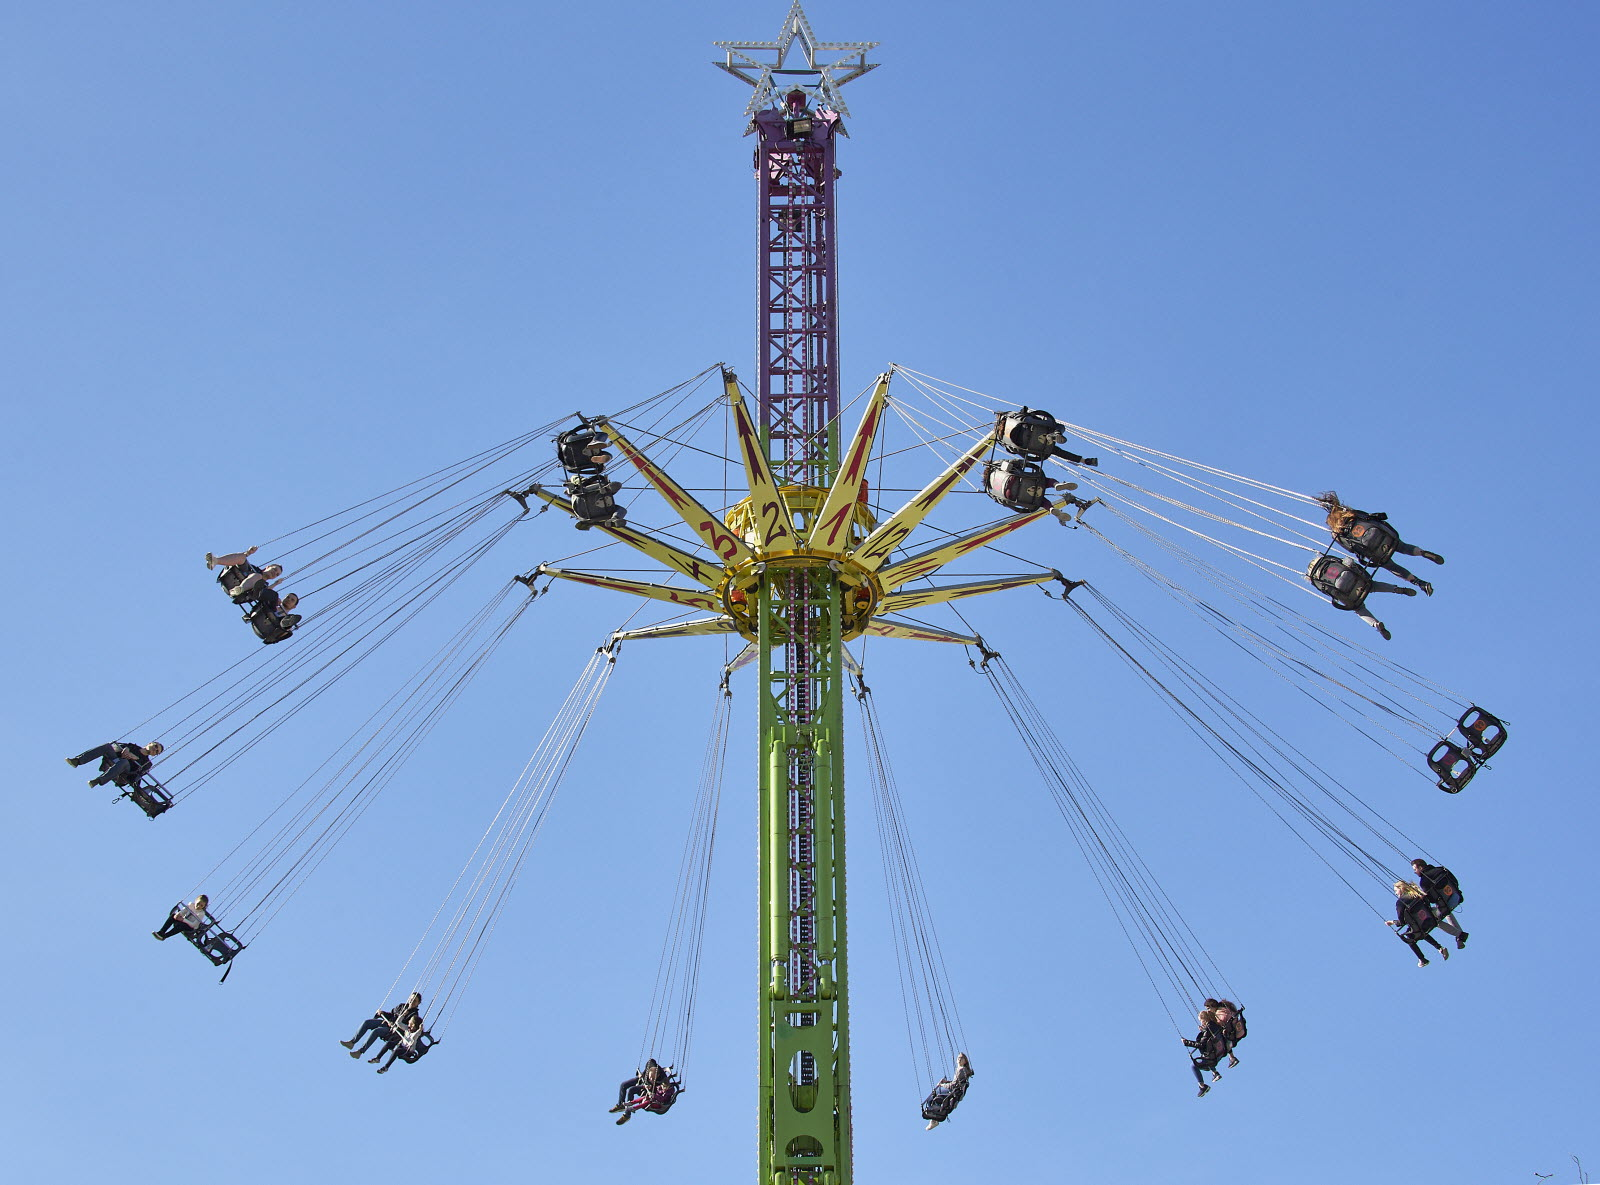
\includegraphics[width=\linewidth]{meca/mecapoint/chaises_volantes.png}
    \caption{Photographie du manège.}
    \label{fig:my_label}
\end{figure}

\textsf{Question ouverte :}~estimer la vitesse de rotation du manège, en rotations par minute.

\end{exercise}

\begin{solution}

Nous allons estimer la vitesse de rotation grâce à la dynamique d'une des chaises volantes, occupée par deux personnes.

Supposant qu'il s'agit d'une particule ponctuelle massive, dans le référentiel tournant, on connaît son accélération centripète due à la rotation $a = -R\Omega^2$. Celle-ci doit être compensée par la projection orthogonale de la force de tension des câbles, elle-même déterminée par la gravité ($g = \SI{9,81}{m^2\cdot s^{-1}}$) dans la direction verticale.

On estime grâce à la référence de taille connue, celle d'une personne assise, environ \SI{1}{m}, on peut estimer la longueur des câbles qui suspendent les chaises volantes : $L = \SI{10}{m}$, ainsi que l'angle entre la verticale et les câbles $\alpha = \SI{45}{deg}$.

On trouve donc :
$$\text{dans la direction $z$} : 0 = -mg + T\cos{\alpha}$$
$$\text{dans la direction $r$} : -mR\Omega^2 = -T\sin{\alpha}$$

Or connaissant également $R = L\sin\alpha$, on obtient :
$\Omega = \sqrt{\dfrac{g}{L\cos\alpha}}$

Ainsi sommes-toute : $\Omega = (\cos\alpha)^{-1/2} = \SI{1.2}{rad\cdot s^{-1}} = \SI{11}{rpm}$.

\end{solution}
% Niveau :      PCSI
% Discipline :  Méca

\begin{exercise}{Bille sur un cerceau}{2}{Sup}
{Mécanique,Ressort}{lelay}


\begin{questions}
    \questioncours Donner l'énergie potentielle correspondant à un ressort de raideur $k$ et de longueur à vide $\ell_0$.

\begin{EnvUplevel}
On considère une bague pesante de masse $m$ glissant sans frottement sur un cercle de rayon $R$, comme sur le schéma ci-dessous.

\begin{center}
    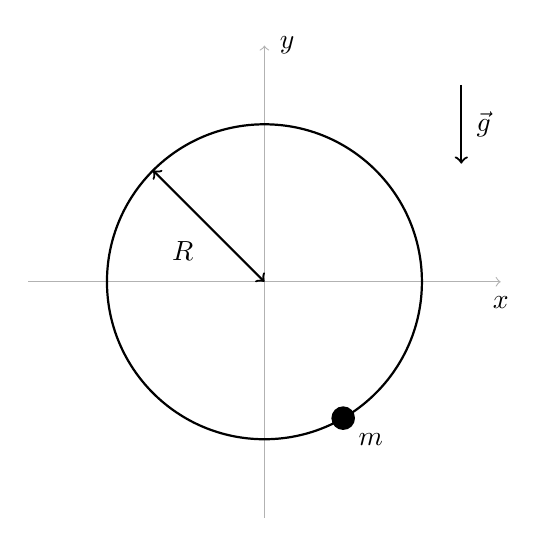
\begin{tikzpicture}
    
    \draw[->, black!30] (-3, 0) -- (3, 0);
    \draw (3,0) node[below=2pt] {$x$};
    
    \draw[->, black!30] (0, -3) -- (0, 3);
    \draw (0,3) node[right=2pt] {$y$};
    
    
    \draw[color=black, thick](0,0) circle (2);
    
    \fill[black] (0.5*2,-0.866*2) circle (0.15);
    \draw (0.5*2,-0.866*2) node[below right=2pt] {$m$};
    
    \draw[<->, thick] (0,0) -- (-0.707*2,0.707*2);
    \draw (-0.707*1,0.707*1) node[below left=2pt] {$R$};
    
    \draw[->, thick] (2.5, 2+0.5) -- (2.5, 2-0.5);
    \draw (2.5,2) node[right=2pt] {$\vec{g}$};
    
    \end{tikzpicture}
\end{center}

\end{EnvUplevel}
    
    \question Donner l'équation du mouvement de la bague. À quel système cette équation vous fait-elle penser ?
    \question En supposant la bille proche du bas du cerceau, quelle approximation permet de linéariser l'équation précédente ? Donner l'équation linéarisée et la famille de solutions correspondante.
    \uplevel{On ajoute maintenant un ressort de raideur $k$ et de longueur à vide $2R$ reliant la bague au point le plus haut du cerceau, comme sur le schéma ci-dessous.}

\begin{center}
    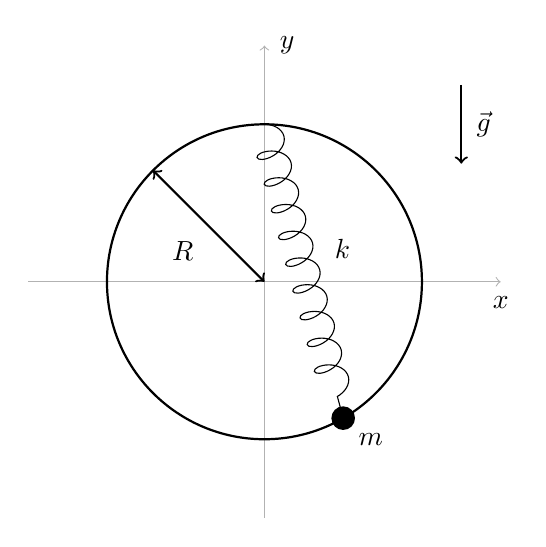
\begin{tikzpicture}
    
    \draw[->, black!30] (-3, 0) -- (3, 0);
    \draw (3,0) node[below=2pt] {$x$};
    
    \draw[->, black!30] (0, -3) -- (0, 3);
    \draw (0,3) node[right=2pt] {$y$};
    
    \draw[color=black, thick](0,0) circle (2);
    
    \fill[black] (0.5*2,-0.866*2) circle (0.15);
    \draw (0.5*2,-0.866*2) node[below right=2pt] {$m$};
    
    \draw[<->, thick] (0,0) -- (-0.707*2,0.707*2);
    \draw (-0.707*1,0.707*1) node[below left=2pt] {$R$};
    
    \draw[->, thick] (2.5, 2+0.5) -- (2.5, 2-0.5);
    \draw (2.5,2) node[right=2pt] {$\vec{g}$};
    
    \draw[decoration={aspect=0.6, segment length=10, amplitude=2mm,coil},decorate] (0,2) -- (0.5*2,-0.866*2);
    \draw (0.7,0.1) node[above right=2pt] {$k$};
    
    \end{tikzpicture}
\end{center}
    \question Donner la nouvelle équation du mouvement de la bague.
    \question En supposant la bille proche du bas du cerceau, développer l'équation jusqu'au premier terme non linéaire. On prendra $k = \frac43 \frac{mg}{R}$.
    \question Quel est l'intérêt de ce dispositif ?

\end{questions}

\end{exercise}

\begin{solution}

\begin{questions}
    \questioncours $E_p = \frac12 k (\ell-\ell_0)^2$
    \question Même dérivation que le pendule (par l'énergie ou la dynamique), on trouve une équation de pendule
    $$ \ddot \theta + {\omega_0}^2\sin \theta = 0$$
    avec $\omega_0 = \sqrt{g / R}$
    \question Équation d'oscillateur harmonique de pulsation $\omega_0$
    \uplevel{On ajoute maintenant un ressort de raideur $k$ et de longueur à vide $\ell_0 = 2R$ reliant la bague au point le plus haut du cerceau, comme sur le schéma ci-dessous.}

    \question 2 possibilités : 
    \begin{itemize}
        \item Rajouter une force de norme $k |\ell - 2R|$. L'angle rajoute un facteur $\sin(\frac\theta2)$.
        
        \item Travailler avec l'énergie mécanique, qui est
    \end{itemize}
    \begin{align*}
    E_m &= E_c + E_{p,g} + E_{p, r} \\
        E_m &= \frac12m R^2\dot{\theta}^2 + mgh + \frac12 k (\ell - 2R)^2
    \end{align*}
    Avec la hauteur $h = - R\cos \theta$ et la longueur du ressort $\ell = 2R \cos(\theta/2)$, d'où
    \begin{align*}
        E_m &= \frac12m R^2\dot{\theta}^2 - mgR\cos\theta + kR (\cos(\theta/2) - 1)^2 \\
        \dd{E_m}/\dd{t} = 0 &= mR^2 \ddot\theta + mgR\sin\theta + 2 kR \sin(\frac{\theta}2)\qty(1 - \cos(\theta/2))
    \end{align*}
    À la fin on doit retomber sur l'équation de la dynamique :
    \begin{align*}
        \ddot{\theta} + \frac{g}{R} \sin\theta + \frac{2k}{m} \sin(\frac{\theta}2)\qty(1 - \cos(\frac{\theta}2)) &= 0
    \end{align*}
    \question À l'ordre 1 le terme supplémentaire ne contribue pas (on a tj un oscillateur harmonique de pulsation $\sqrt{g/L}$). Surprise, les termes d'ordre 3 s'annulent ! Il reste des termes d'ordre 5.
    \question On a réussi à compenser la première non linéarité, on a donc des oscillations plus isochrones

\end{questions}
\end{solution}
% Niveau :      PCSI
% Discipline :  Mécanique
%Mots clés :    Météorite, pénétration

\begin{exercise}{Profondeur d'impact}{1}{Sup}
{Mécanique}{lelay}

On s'intéresse à la profondeur maximale de pénétration d'un objet lancé avec une vitesse initiale dans un milieu, comme par exemple dans le cas d'une météorite qui tomberait sur Terre.
\begin{questions}
    \question \textbf{Approche naïve.} On considère d'abord une approche naïve (appelée sur wikipédia "approche de Newton", cette approche a en fait été développée par Gamov en 1961 -- comme quoi il ne faut pas croire tout ce qu'on lit sur internet). On considère une objet de masse $m$ et de densité $\mu_m$ pénétrant dans un milieu de densité $\mu$ avec une vitesse initiale $v_0$. L'objet est supposé être de section $A$ et de longueur $\ell$.
        \begin{parts}
            \part Cette approche considère la pénétration dans les solides et les fluides de la même manière. Cela vous paraît-il raisonnable ? En fait ce n'est pas aberrant, car à partir d'une certaine vitesse d'impact les solides se comportent comme des fluides. Quelle est à votre avis cette vitesse ? En donner des ordres de grandeur dans différents milieux.
            \part En ne considérant que la quantité de mouvement, Gamov suppose que l'objet déplace le milieu à la vitesse à laquelle il se déplace, et que l'objet s'arrête après avoir transmis toute sa quantité de mouvement au milieu. Montrer que le profondeur de pénétration (la distance au bout de laquelle l'objet s'arrête) est alors $L = \ell \frac{\mu_m}{\mu}$
            \part Interpréter les termes de l'équation obtenue. Cela vous parait-il logique ? Quelles sont les limites de cette approximation ?
            \part En utilisant cette approximation, donner la portée d'une balle de .22 LR (15 mm de long, c'est le calibre de beaucoup de petites armes au poing dont celle utilisée par James Bond) dans l'air, puis dans l'eau. Justifier qu'on puisse arrêter une balle de ce pistolet en tirant dans un verre d'eau. Disserter longuement sur le fait que les adversaires de James Bond auraient gagné à se placer derrière un aquarium. 
            \part L'astéroïde de Chicxulub, au Mexique (celui qui a tué les dinosaures), avait une taille estimée entre 11 et 80 km. Le cratère de Chicxulub est large de plus de 150 km mais n'est profond que de 20 km. Est-ce cohérent avec l'analyse développée ci-dessus ?
        \end{parts}
    \question \textbf{Cas des fluides} Ici on considère la véritable approche de Newton dans les \textit{Principia} (livre 2, section 7), qui traitait du cas spécifique des fluides. Newton a conclu de ses expérience sur l'amortissement des oscillations d'un pendule que les deux principales forces ralentissant un objet passant dans un fluide étaient linéaires et quadratiques en la vitesse de l'objet.
        \begin{parts}
            \part Que savez-vous de ces forces de frottement fluide ? Quelle est celle qui prévaut à grande vitesse ? A faible vitesse ? Bonus : comment quantifier "faible vitesse" et "grande vitesse" dans ce cas ?
            \part En considérant un solide de masse $m$ et de vitesse initiale $v_0$ soumis uniquement à une force quadratique en la vitesse $F_Q = -\beta v^2$, montrez que cette force ne suffit pas pour que le solide s'arrête. Astuce : écrivez la PFD en utilisant $\dv{v}{x}$.
            \part En considérant cette fois la force quadratique précédente et une force linéaire en la vitesse $F_L = - \alpha v$, montrez que la distance d'arrêt est $L = \frac{m}{\beta}\ln{1+\frac{\beta}{\alpha}v_0}$.
            \part Sans intégrer ou dériver d'équation, donner la distance d'arrêt pour la force linéaire seule.
            \part En considérant comme on le fait classiquement que $\beta$ dépend linéairement de la surface frontale du l'objet et de la densité du milieu, montrer qu'on retrouve le résultat de la section précédente à un facteur sans dimension près.
        \end{parts}
    
    \pagebreak
    
    \question \textbf{Cas des solides} On s'intéresse maintenant au cas de l'impact d'objets dans des solides, tel qu'étudié par Young, ingénieur américain dans les années 60.
        \begin{parts}
            \part Young considère dans un premier temps qu'un objet s'enfonçant dans un milieu solide (comme la terre ou l'argile) est soumis à une force $F = F_0 + k v^2$. En intégrant le PFD, montrez qu'on obtient une profondeur de pénétration $L = \frac{m}{2k}\ln{1+\frac{k}{F_0}v_0^2}$
            \part Young trouvait son modèle peu fiable, il a donc fait beaucoup d'expériences et a trouvé que la profondeur était en fait donnée par $L = \sqrt{\frac{m}{A}}v_0\ln{1+jv_0^2}S$, où $A$ est la surface en coupe de l'objet, $j$ un facteur numérique et $S$ une constante dépendant du type de sol. Quelle est la dimension de $S$ ?
        \end{parts}
    
\end{questions}

\end{exercise}

\begin{solution}

% \question \textbf{Approche naïve.}
%     \begin{parts}
%         \part Vitesse du son.
%         \part qté de mvt de initiale : $\ell A \rho_m v_0$ (l'objet), qté de mvt finale : $L A \rho v_0$ (le milieu)
%         \part Là il faut dire que c'est bizarre parce qu'il n'y a pas la vitesse, donc ça ne doit pas marcher pour tous les régimes.
%         \part On trouve une dizaine de centimètres. Aux US Mythbusters on fait l'expérience, en tirant dans un verre d'eau plein depuis le dessus, et ils ne l'ont pas cassé.
%         \part Oui, la profondeur est de l'ordre de la taille de l'astéroïde. La taille du cratère montre que son énergie s'est dissipée latéralement et pas en profondeur
%     \end{parts}
% \question \textbf{Cas des fluides}
%     \begin{parts}
%         \part linéaire, quadratique. Pour le bonus : c'est le nombre de Reynolds bien sûr
%         \part Là il faut juste qu'il trouvent que $\dv{v}{t} = v\dv{v}{x}$, le reste est trivial.
%         \part Pareil, trivial
%         \part On fait tendre $\beta$ vers 0 et on fait un DL
%         \part prout. Si ils écrivent $\beta = A \rho k$ avec $k$ une constante, demander quelle est la dimension de $k$
%     \end{parts}
% \question \textbf{Cas des solides} 
%     \begin{parts}
%         \part C'est comme dans la partie d'avant
%         \part C'est chiant, les ingénieurs sont des relous avec leurs racines de $m$ à la mord-moi-le-noeud
%     \end{parts}

\end{solution}
\begin{exercise}{La fusée}{2}{Sup, Spé}
{Mécanique,PFD}{lelay}

\begin{questions}
    \questioncours Rappeler la seconde loi de Newton.
    \question Soit une fusée qui est propulsée en évacuant en permanence vers le bas du carburant (avec un débit $Q$)  à la vitesse $v_\text{e}$. Faire un schéma de la fusée à $t$ et $t+\dd{t}$
    \question Appliquer le second principe de Newton à la fusée, en déduire une expression de $\dv{v}{t}$.
    \question Proposer une modélisation de la masse de la fusée $m(t)$
    \question Donner $v(t)$. Quelle est la vitesse atteinte par la fusée une fois tout son carburant largué ? Comment optimiser cette vitesse ?
    \question Donner $x(t)$. Quelle est la hauteur finale atteinte par la fusée ?
    \question Faire des applications numériques sachant qu'une fusée Ariane 5 pèse 750 tonnes au décollage, que 97.5\% de cette masse consiste en du carburant, et que sa phase d'accélération dure environ 500s.
    \question Une de nos approximations est-elle remise en cause ? Proposer un moyen de résoudre ce problème.
\end{questions}
\end{exercise}

\begin{solution}


\begin{questions}
    \questioncours $F=ma$
    \question F F 
    \question $p(t) = m(t) v(t)$ et $p(t+\dd{t}) = m(t+\dd{t})v(t+\dd{t}) + (-\dd{m})(v(t)-v_e)$ (car la petite masse éjectée est $\delta m = - \dd{m}$ d'où $\dv{p}{t} = \dv{mv}{t} - \dv{m}{t}(v-v_e) = m\dv{v}{t} + v_e\dv{m}{t}$ or $\dv{p}{t} = -m(t)g$ (PFD) d'où $\dv{v}{t} = \qty( - g - \frac{v_e}{m}\dv{m}{t})$
    \question $m(t) = m_0 - Qt$ puis $m = m_f$ à partir de $t_f = \frac{m_0-m_f}{Q}$
    \question $\dv{v}{t} = \qty( -g + \frac{Qv_e}{m_0 - Qt})$. On intègre pour trouver $v(t_f) = -\frac{g m_0}{Q}\qty(1-\frac{m_f}{m_0}) + v_e\ln(\frac{m_0}{m_f})$ (à contre-checker)
    \question La primitive de $\ln(x+a)$ est $(x+a)\ln(x+a) - x$ (changement de variable)
    \question On trouve une hauteur où la gravité est faible ? Ai pas fait le calcul lol.
    \question On a supposé $g$ constant...
\end{questions}

\end{solution}
% Niveau :      PC *
% Discipline :  Méca
% Mots clés :   Lune

\begin{exercise}{Formule de Borda}{3}{Sup, Spé}
{Mécanique,Mécanique du point,Pendule}{bermu}

\begin{questions}
\questioncours pendule simple idéal pour de faibles amplitudes. On explicitera sa fréquence propre $\omega_0$ et sa période propre $T_0$. On se placera dans les coordonnées polaires $(r, \theta)$.
\question On étudie maintenant un pendule réel.
\begin{parts}
\part Quels phénomènes (on en citera au moins deux) ne sont pas traduits par le modèle de
l’oscillateur harmonique ? 
\part Tracer le portrait de phase du pendule simple idéal, puis réel, dans ces différentes configurations.

\textbf{Rappel :} le portrait de phase d'un système est le graphique représentant la vitesse en fonction de la position pour différentes conditions initiales.
\end{parts}
\question On se place désormais dans le cas général d’un régime lié sans frottements.
\begin{parts}
\part En utilisant la conservation de l’énergie mécanique, exprimer $\dot{\theta}(t)$ en fonction de $\theta(t)$ et $\theta_0=\theta(0)$.
\part En déduire une expression de $T$, la période du pendule (dans le cas général) en fonction de
$T_0$ et $\theta_0$ en utilisant la fonction elliptique $K$
$$K(m) = \dfrac{2}{\pi}\int_0^{\pi/2} \dfrac{\dd{\phi}}{1 - m \sin^2\phi}.$$
\part Linéariser l’expression pour de petits angles, et en déduire la formule de Borda :
$$T = T_0\qty(1 + \dfrac{{\theta_0}^2}{16}).$$
On pourra s'aider de la relation suivante sur les intégrales de Wallis
$$W_{2n} = \int_0^{\pi/2} \sin^{2n}\phi \dd{\phi} = \dfrac{\pi}{2} \dfrac{(2n)!}{(2^n n!)^2},$$
$$W_0 = \dfrac{\pi}{2}, \quad W_2 = \dfrac{\pi}{4}, \quad W_4 = \dfrac{3\pi}{16}, \quad W_6 = \dfrac{5\pi}{32}\  \ldots$$
Commenter au regard du portrait de phase.
\part Évaluer le domaine de validité de cette expression.
\end{parts}
\end{questions}

\paragraph{Donnée :}~\vspace{-3em}\\
\begin{figure}[H]
    \centering
    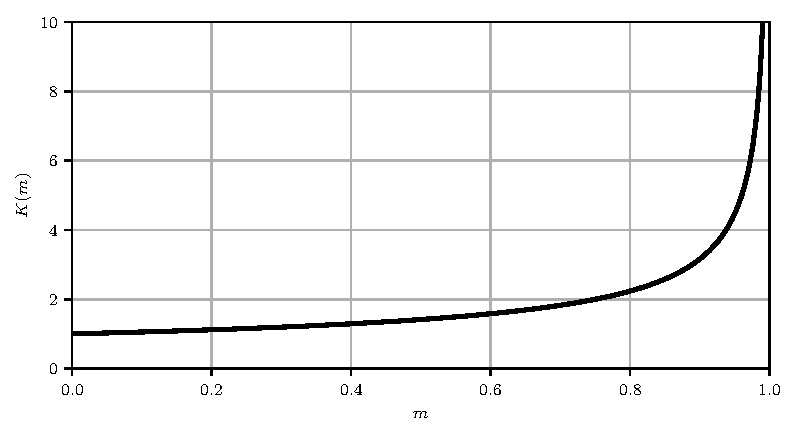
\includegraphics[scale=1]{meca/fonction_K.pdf}
    \vspace{-2em}
    \caption{Graphe de la fonction $K(m)$.}
\end{figure}
\end{exercise}

\begin{solution}
\begin{questions}
    \questioncours \'Equation du pendule $\Ddot{\theta} - k/m\sin\theta = 0$ d'où $\omega_0 = \sqrt{\dfrac{k}{m}}$.
    \question\begin{parts}
        \part Non linéarité et frottements.
        \part Idéal : cercles concentriques, réel sans frottement : des ovales rigolos, réel avec frottement : des spirales cheloues.
    \end{parts}
    \question\begin{parts}
        \part TMC depuis l'équation du pendule
        $$\dfrac{1}{2}\dv{}{t}\qty(\dot{\theta}^2) - {\omega_0}^2\sin\theta\dv{\theta}{t} = 0$$
        et par intégrale première du mouvement entre $\theta = \theta_0$ et $\theta(t)$ :
        $$\dot{\theta} = \omega_0\sqrt{\cos\theta_0 - \cos\theta}.$$
        \part D'où par intégration entre $0$ et $T/4$ et $0$ et $\theta_0$ :
        $$T = \dfrac{2T_0}{\pi}\int_{0}^{\theta_0}\dfrac{\dd{t}}{\sqrt{\cos\theta_0 - \cos\theta}}.$$
        et avec le changement de variable $\sin\phi = \dfrac{\sin(\theta/2)}{\sin(\theta_0/2)}$, on trouve $T = T_0 K(\sin^2(\theta_0)/2).$
        \part Pour $m$ petit,
        $$\frac{1}{\sqrt{1-m\sin^{2}\phi}}=1+\frac{\sin^{2}\phi}{2}m+\mathcal{O}(m^2\sin^{4}\phi),$$
        d'où par intégration on retrouve la formule de Borda.
        \part Le terme suivant, et on fait un critère.
    \end{parts}
\end{questions}
\end{solution}
% Niveau :      PC
% Discipline :  Méca
% Mots clés :   Van Der Pol

\begin{exercise}{Oscillateur Van Der Pol}{3}{Spé}
{Mécanique, Oscillateur harmonique, Pendule, Référentiel non galiléen}{lelay}

Il est possible en utilisant le montages montré sur l'image ci-dessous de faire en sorte que deux pendules se synchronisent : 

{\centering
    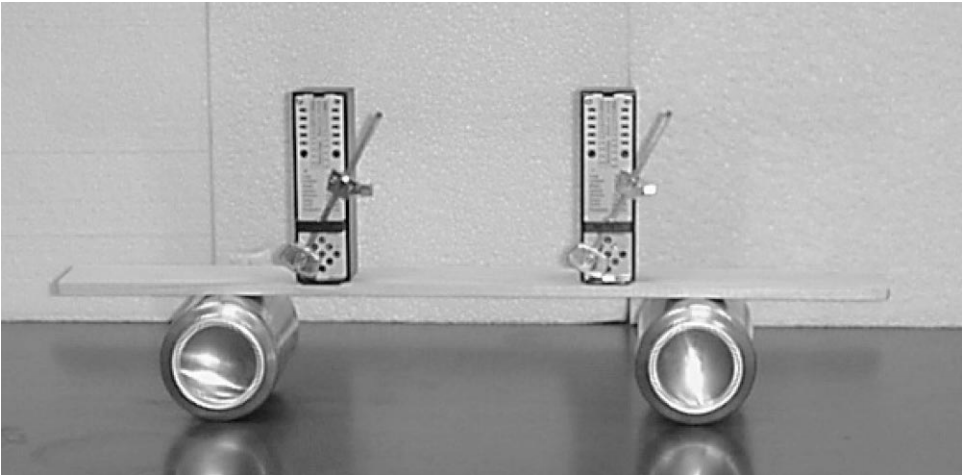
\includegraphics[scale=0.3]{meca/mecapoint/vanderpol.png}\par
}

Pour cet exercice, on considérera que les pendules sont auto-entretenus, que les canettes roulent sans glissement et que le mouvement d'un pendule auto-entretenu seul (sur une base fixe) est régi par l'équation dite de Van Der Pol : 
\begin{align*}
\frac{\dd^2 \theta}{\dd t^2} + \frac{g}L\sin\theta + \varepsilon\qty(\qty(\frac\theta{\theta_0})^2-1)\frac{\dd \theta}{\dd t}=0
\end{align*}

\begin{questions}
    \question Expliquer l'origine physique de chacun des termes de l'équation ci dessus.
    \question Justifier qu'un pendule obéissant à l'équation ci-dessus peut avoir un mouvement périodique d'amplitude constante. [Bonus : Le démontrer.]
	\question Établir l'équation du mouvement des deux pendules 
	\question Montrer qu'il peut y avoir synchronisation des pendules
\end{questions}
\end{exercise}
% Niveau :      PCSI
% Discipline :  Méca

\begin{exercise}{Bifurcation fourche supercritique}{3}{Sup}
{Mécanique,Ressort}{lelay}

On considère une bille de masse $m$ glissant sans frottement sur un rail (l'axe $Ox$) accrochée par un ressort de raideur $k$ et de longueur à vide $\ell_0$ placé à une distance $a$ du rail.
\begin{questions}
    \questioncours Rappeler la définition de point d'équilibre en mécanique
    \question À votre avis, quel va être le mouvement de la bille ? Comment va-t-il évoluer en fonction des paramètres du problème ?
    \question Par la méthode de votre choix, trouver les points d'équilibre de la bille. Combien y en a-t-il ?
    \question Représenter sur un graphe les points d'équilibres (sous forme adimensionnée $u=x_{eq}/a$) en fonction de $r = \ell_0/a$.
    \question On s'intéresse maintenant à la stabilité de ces points d'équilibre. Rappeler comment déterminer la stabilité d'un point d'équilibre. 
    \begin{parts}
        \part On considère le cas $a > \ell_0$. Combien de points d'équilibre y a-t-il ? Quelle est leur stabilité ?
        \part On considère le cas $a < \ell_0$. Combien de points d'équilibre y a-t-il ? Quelle est leur stabilité ?
        \part Redessiner le graphe $u = f(r)$ en prenant compte de la stabilité des points. Pourquoi appelle-t-on cette bifurcation \textit{fourche} supercritique ?
    \end{parts}
    \uplevel{\slshape Vous pouvez choisir de faire les deux prochaines question dans l'ordre que vous souhaitez.}
    \question\textsf{Le noeud du problème (\emph{Calculatoire})}.
    \begin{parts}
        \part Dans le cas où $\ell_0 = a$, combien y-a-t-il de points d'équilibre ? Sans calcul, ce point d'équilibre est-il stable ? 
        \part Écrire le PFD au premier ordre non nul en $x$ près du point d'équilibre. Connaissez vous une solution à cette équation différentielle ?
        \part Tracer le portrait de phase correspondant à cette équation, en déduire que le point d'équilibre est stable. \\
        \textbf{Rappel :} le portrait de phase d'un système est le graphique représentant la vitesse en fonction de la position pour différentes conditions initiales.
        \part En supposant que initialement on a $x = x_0$ et $\dot x = 0$, exprimer la période des oscillations en fonction des paramètres du problème et de l'intégrale
        \begin{align*}
        I &= \int_{-1}^1\frac{dy}{\sqrt{1-y^4}} \approx 2.62
        \end{align*}
        \part Proposer des valeurs pour $m$, $k$, $a$ et $x_0$ et calculer $T$.
    \end{parts}
    \question\textsf{La théorie des catastrophes.}
    \begin{parts}
        \part On suppose maintenant que le rail est incliné d'un angle $\alpha$ par rapport à l'horizontale. Montrer que l'équation que vérifient les points fixes donne sous forme adimensionnée :
        \begin{align*}
            1+\frac{h}u = \frac{r}{\sqrt{1+u^2}}
        \end{align*}
        où $h$ est une constante à déterminer.
        \part En supposant $u \ll 1$, montrer que cette équation se réduit à $u^3+h = (r-1)u$. En prenant $h \ll 1$, dessiner les graphes des fonctions $u \mapsto u^3+h$ et $u\mapsto (r-1)u$ pour $r > 1$ et $r<1$. 
        \part En déduire l'allure du graphe $u = f(r)$. Qu'est ce qui a changé par rapport à la situation précédente ? 
        \part Pour un $r>1$ donné, représenter l'allure de $u = f(h)$. Pouvez-vous expliquer pourquoi cette bifurcation est \textit{catastrophique} ?
    \end{parts}

\end{questions}
 \plusloin La théorie des bifurcations est une étape importante pour l'étude des objets complexes, par exemple les systèmes physiques modélisés par des équations non linéaires.
    
% \begin{figure}{H}
%     \centering
%     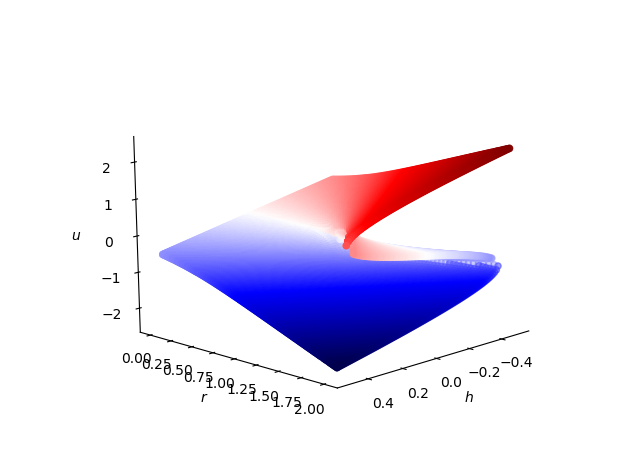
\includegraphics[height=15em]{meca/mecapoint/fourchevraie.png}
%     \caption{Vision pas d'artiste d'une bifurcation fourche supercritique.}
% \end{figure}

% \begin{figure}{H}
%     \centering
%     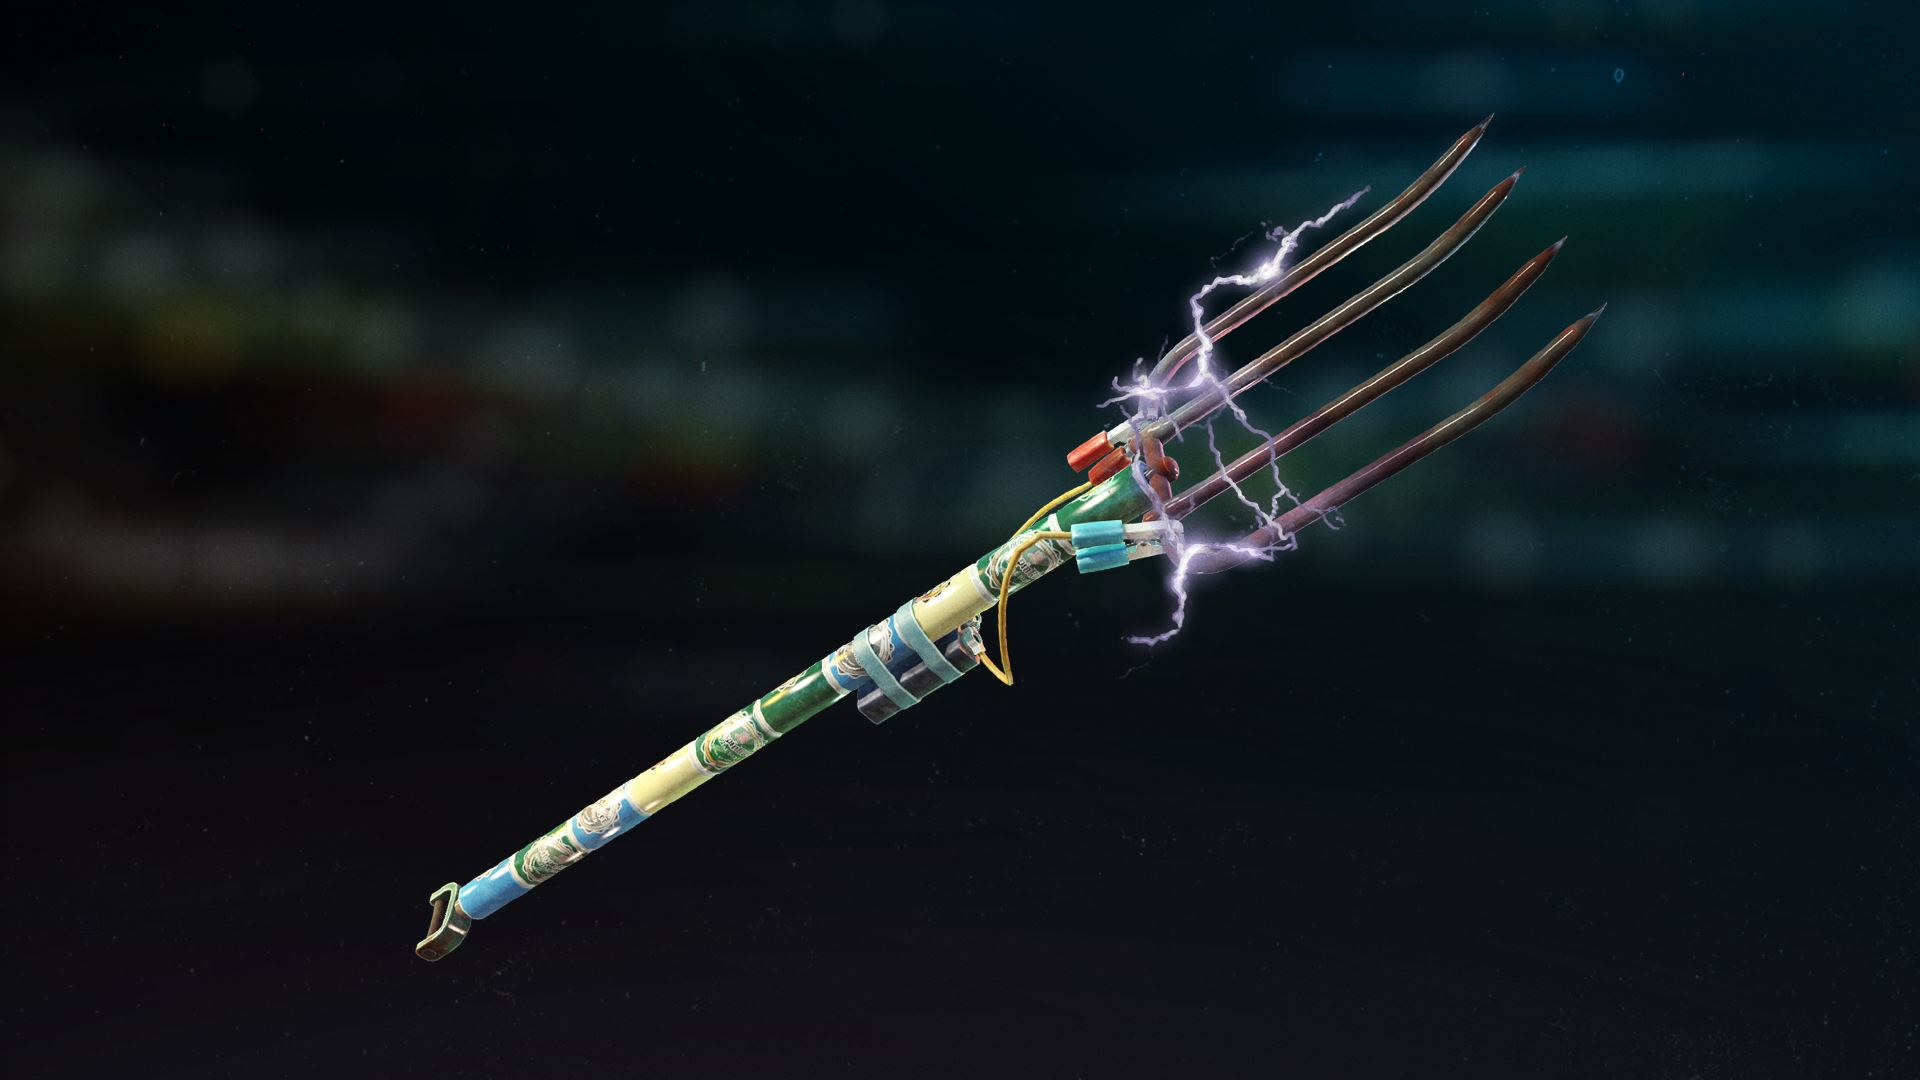
\includegraphics[height=15em]{meca/mecapoint/fourchesupercritique.jpg}%non ! siii ! %gros vilain !
%     \caption{Vision d'artiste d'une fourche supercritique.}
% \end{figure}

\end{exercise}
% Niveau :      PC **
% Discipline :  Méca
% Mots clés :   Brachistochrone, moindre action

\begin{exercise}{Brachistochrone}{4}{Spé}
{Mécanique,Mécanique du point}{bermu}

La brachistochrone (de \emph{chronos} le temps, \emph{brakhistos} le plus court) est la trajectoire la plus rapide (en temps) d’un point $A$ à un point $B$.
\begin{questions}
\question Décrire plusieurs situations où la brachistochrone n’est pas la droite $AB$, c'est à dire où le chemin le plus court n'est pas le plus rapide. \\
\textbf{Indice :} On pourra observer une masse $m$ dans un champ de pesanteur $g$ ayant pour trajectoires
\begin{parts}
\part la droite $AB$, \part un arc de cercle, \part une chute verticale un mouvement horizontal...
\end{parts}
\question Analogie avec l'optique.
\begin{parts}
\part Énoncer un principe optique analogue à celui de la brachistochrone.
\part \`A l’interface de deux milieux optiques, quelle loi caractérise ce principe ? Démontrer cette loi.

Supposons maintenant que le milieu soit à gradient d’indice optique $n(z)$.
\part En utilisant la loi précédente, exprimer en fonction de $\theta$, l’angle de la tangente à la trajectoire par rapport à l’axe $\hat{u}_z$, et de $n(z)$ une quantité qui se conserve sur le rayon lumineux.\\
Tracer qualitativement le rayon dans un cas simple.
\end{parts}
\question Retour sur la brachistochrone :
On considère une masse m dans un champ de pesanteur g
\begin{parts}
\part Donner une relation entre la vitesse v, et l’altitude z de m.
\part Par analogie avec la question 2c), donner une relation entre l’angle $\theta$ et l’altitude $z$.
\part Montrer qu’une cycloïde vérifie une telle relation et déduire l’équation de la cycloïde. Tracer cette trajectoire et la comparer aux trajectoires étudiées en 1. \\
\textbf{Donnée :} une cycloïde est la trajectoire d’un point fixé à un cercle qui roule sans glisser sur une droite qui
peut être paramétrée de la manière suivante :
$$\left\{\mqty{x(\nu) = R(\nu - \cos\nu) \\ z(\nu) = R(1 - \sin\nu)}\right., \nu\in[0,\pi].$$
\end{parts}
\end{questions}

\plusloin
On peut également montrer que la brachistochrone est aussi une tautochrone (de \emph{chronos} le temps, \emph{tautos} ) c’est-à-dire une courbe telle que tout point matériel lâché sans vitesse initiale sur la courbe arrive en un point donné en un temps indépendant du point de départ.

\end{exercise}
% Niveau :      PCSI *
% Discipline :  Méca
% Mots clés :   Ballistique, Mécanique du point, PFD, Chute libre

\begin{exercise}{Variations sur le looping}{2}{Sup, Spé}
{Mécanique,Mécanique du point}{bedo,bermu}

\begin{questions}
\questioncours Lois du frottement solide.

\bigskip

\question\textsf{Question ouverte :} On considère une bille dans un champ de pesanteur lancée avec une certaine vitesse horizontale. La bille est contrainte d'adopter une trajectoire lui faisant faire un looping.

\'Etudier la différence entre les trois situations suivantes :
\begin{enumerate}[label={\bfseries \sffamily (a)}]
    \item la bille est une perle enfilée dans un circuit rigide en forme de cercle ;
    \item la bille roule dans une gouttière circulaire ;
    \item la bille est attaché à une corde non rigide et non élastique.
\end{enumerate}

\end{questions}

\paragraph{Conseils méthodologiques :}
\begin{itemize}
    \item \textsl{Schématiser ces situations et poser les grandeurs physiques qui vous paraissent importantes} ;
    \item \textsl{\'Etudier qualitativement les trois situations et identifier les différences} ;
    \item \textsl{Faire les calculs pour chaque situations} ;
    \item \textsl{Conclure}.
\end{itemize}

\end{exercise}

% Niveau :      PCSI
% Discipline :  Méca

\begin{exercise}{Flambage}{3}{Sup}
{Mécanique,Ressort}{lelay}

\textsl{Le but de cet exercice est de modéliser de manière simple l'instabilité de flambage. C'est ce qui se produit par exemple lorsqu'on compresse une règle en plastique à ses extrémités.}

On considère deux murs verticaux situés en $x = \pm a$. Une masse $m$ est reliée à chacun des murs par un ressort de raideur $k$ et de longueur à vide $\ell_0$ dont les points d'attache sont situés face à face.
\begin{questions}
    \questioncours Définition d'un point d'équilibre stable, instable.
    \question Montrez qualitativement que si la masse est initialement centrée en $x=0$, elle y restera tout le temps. On considérera cette condition comme vérifiée par la suite.
    \uplevel{On considère dans un premier temps que la masse n'est pas soumise à son poids ($g = 0$).}
    \question On considère le cas $a > \ell_0$. Appliquer le PFD à la masse.
    \begin{parts}
        \part Combien y a-t-il de points d'équilibre ?
        \part Donner l'équation horaire du mouvement de la masse en considérant qu'elle commence son mouvement à $t=0$ proche d'un point d'équilibre et sans vitesse initiale.
    \end{parts}
    \question On considère le cas $a < \ell_0$. Écrire l'énergie potentielle de la masse.
    \begin{parts}
        \part Combien y a-t-il de points d'équilibre ?
        \part Donner l'équation horaire du mouvement de la masse en considérant qu'elle commence son mouvement à $t=0$ proche d'un point d'équilibre et sans vitesse initiale.
    \end{parts}
    \question Représenter sur un graphe les points d'équilibres (sous forme adimensionnée $u=z_{eq}/\ell_0$) en fonction de $r = a/\ell_0$.
    \question On s'intéresse maintenant à la stabilité de ces points d'équilibre. Rappeler comment déterminer la stabilité d'un point d'équilibre. 
    \begin{parts}
        \part On considère le cas $a > \ell_0$. Combien de points d'équilibre y a-t-il ? Quelle est leur stabilité ?
        \part On considère le cas $a < \ell_0$. Combien de points d'équilibre y a-t-il ? Quelle est leur stabilité ?
        \part Redessiner le graphe $u = f(r)$ en prenant compte de la stabilité des points. Pourquoi appelle-t-on cette bifurcation \textit{fourche} super critique ?
    \end{parts}
    \uplevel{On considère maintenant que la bille est soumise à son poids ($g \neq 0$).}
    \question À votre avis, qu'est-ce que cela va changer au problème ? 
    \question On considère une bille de faible poids. Comment quantifier physique cette affirmation ?
    \begin{parts}
        \part On suppose maintenant que le rail est incliné d'un angle $\alpha$ par rapport à l'horizontale. Montrer que l'équation que vérifient les points fixes donne sous forme adimensionnée :
        \begin{align*}
            1+\frac{h}u = \frac{r}{\sqrt{1+u^2}}
        \end{align*}
        où $h$ est une constante à déterminer.
        \part En supposant $u \ll 1$, montrer que cette équation se réduit à $\frac{u^3}{2r^3}+h = \frac{1-r}{r}u$. En prenant $h \ll 1$, dessiner les graphes des fonctions $u \mapsto u^3+h$ et $u\mapsto (r-1)u$ pour $r > 1$ et $r<1$. 
        \part En déduire l'allure du graphe $u = f(r)$. Qu'est ce qui a changé par rapport à la situation précédente ? 
        \part Pour un $r>1$ donné, représenter l'allure de $u = f(h)$. Pouvez-vous expliquer pourquoi l'ajout de $g$ est \textit{catastrophique} ?
    \end{parts}
    \question Que se passe-t-il  si $g$ est grand ?
\end{questions}

% \begin{figure}{H}
%     \centering
%     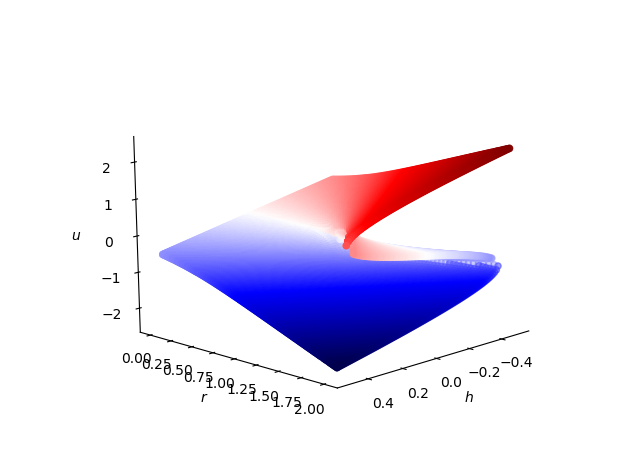
\includegraphics[height=15em]{meca/mecapoint/fourchevraie.png}
%     \caption{Vision pas d'artiste d'une bifurcation fourche supercritique.}
% \end{figure}

% \begin{figure}{H}
%     \centering
%     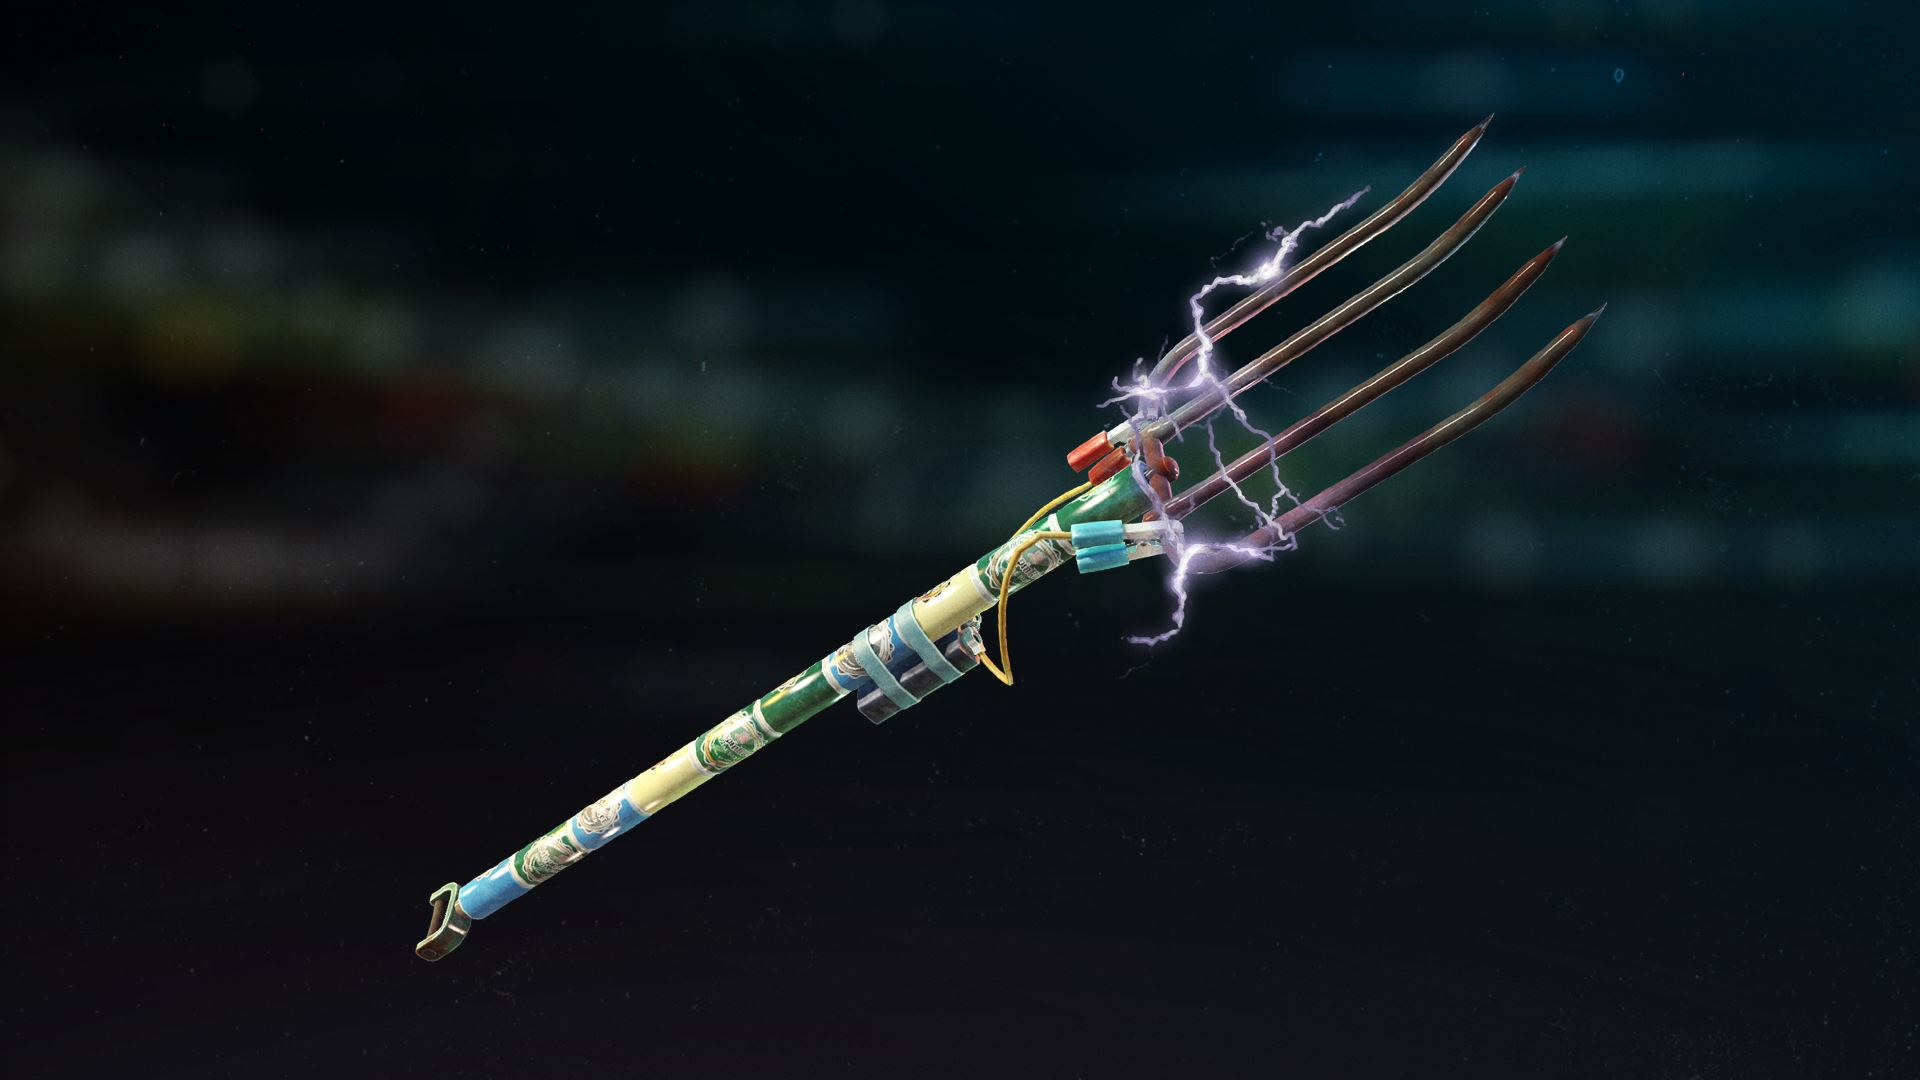
\includegraphics[height=15em]{meca/mecapoint/fourchesupercritique.jpg}%non ! siii ! %gros vilain !
%     \caption{Vision d'artiste d'une fourche supercritique.}
% \end{figure}

\end{exercise}
\begin{exercise}{Distance au firmament}{2}{Sup, Spé}
{Mécanique,Mécanique du point}{lelay}

Xénophanes de Colophon, auteur grec de l'antiquité, affirmait que les étoiles étaient fixes et collées sur une grande surface semi-sphérique qu'il appelait firmament. Hésiode, à la même époque, précise la distance entre la surface de la Terre et le firmament en affirmant qu'un enclume lâchée depuis les étoiles mettrait neuf jours et autant de nuits à atteindre la Terre.  

\begin{questions}
    \questioncours Intégrale première du mouvement
    \question On suppose d'abord que l'accélération de la pesanteur est constante égale à $g$. Déterminer la distance entre les étoiles et la surface de la Terre d'après Hésiode. Cela vous paraît-il réaliste ?
    \question On suppose maintenant que la force de gravité s'exerçant sur l'enclume est la force générale de gravitation due à la Terre. Estimer la distance totale parcourue par l'enclume.
    \question Comparer aux autres distances du système solaire : Distance Terre Lune 384 000 km, distance Terre Mras 306 millions de km
\end{questions}

Données : On donne $\int \frac{\dd{x}}{\sqrt{\frac1x-1}} = -x\sqrt{\frac1x-1} - \arctan(\sqrt{\frac1x-1})$
\end{exercise} 

\section{Particules chargées}
% Niveau :      PCSI *
% Discipline :  Méca
% Mots clés :   Trajectoire particule chargée

\begin{exercise}{Arc électrique : c'est disruptif !}{2}{Sup, Spé}
{Mécanique,Mécanique particules chargées,Thermodynamique}{bermu}

\begin{questions}
\questioncours Quelle est la définition de l'électron-volt eV et dans quels cas l'utilise-t-on ?

\begin{EnvUplevel}
On se propose d'étudier une décharge électrique entre deux électrodes planes séparées d'une distance $d = 10$ mm et donc la différence de potentiel est $V_0 = 1$ kV. Le problème étant quasi 1D, on ne regardera que la variable d'espace $x$.
\end{EnvUplevel}

\question Quelle est l'expression du potentiel $V$ et du champ électrique $\vE$ entre les deux électrodes ?

\question Quelle est la trajectoire d'un seul électron en fonction du temps ? Cela vous paraît-il réaliste ?

\uplevel{La décharge électrique est créée par un phénomène d'\emph{avalanche électronique} : à chaque collision avec un atome d'air, un électron arrache un électron à l'atome qui lui-même arrache d'autres électrons \textit{etc}.}

\question Entre deux collisions, l'électron parcours une distance $\ell$ correspondant au libre parcours moyen dans le gaz. Supposant qu'il soit réémis suivant $Ox$, quelle est la vitesse moyenne $v_m$ de l'électron ?

%\question Et s'il était réémis dans des directions aléatoires ? (\emph{Vous pouvez seulement entamer la démarche sans faire les calculs.})

\question Sachant qu'il faut un travail $W_\text{ion}$ pour arracher un électron, donner un critère sur $V_0$ et le libre parcours moyen $\ell$ du gaz pour qu'il y ait une avalanche électronique. \\
Calculer $V_0$. Cela vous parait-il cohérent ?

\question Combien d'électrons auront été émis après un temps $t$ ? En déduire que la loi de courant des électrons est exponentielle
$$\vj_e = j_0 e^{\alpha x}\ve_x,$$
$j_0$ et $\alpha$ étant des paramètres que vous identifierez.

\uplevel{La décharge électrique étant aussi liée au courant des ions il faut également prendre en compte la dynamique des ions.}

\question Comment se comportent les ions ? Donner l'énergie cinétique des ions lorsqu'ils arrivent en $z=0$ et comparer à $W_\text{ion}$.

\uplevel{Cette vitesse étant très grande, cela signifie que les ions arrachent également des électrons à la cathode.}

\question Estimer le nombre $\gamma$ d'électrons arrachés par  un ion.

\question Justifier que
$$j(0) = \gamma\qty(j(0) - j(d)),$$
et en déduire la loi de Townsend
$$j(d) = j(0) \dfrac{e^{\alpha d}}{1 + \gamma(1 - e^{\alpha d})}.$$

\question Cette loi admet une singularité : donner la relation entre $\alpha$ et $\gamma$ à la singularité et interpréter physiquement la singularité.
\question En déduire la loi de Paschen :
$$V_\text{disruption} = U_\text{ion}\dfrac{d/\ell}{\ln{d/\ell} - \ln(1+\gamma^{-1})}.$$
Quelle est la tension de disruption du système ?
\end{questions}

\paragraph{Données :}
\begin{itemize}
    \item charge élémentaire $e = 1,6\times 10^{-19}$ C,
    \item masse le l'électron $m_e = 9,1\times 10^{-31}$ kg,
    \item masse d'un ion $m_i = 2,6\times 10^{-26}$ kg,
    \item dans l'air sec : $W_\text{ion} = 34$ V et $\ell = 70$ nm.
\end{itemize}
\end{exercise} 
\begin{exercise}{Piège de Penning}{2}{Spé}
{Magnétostatique}{lelay}

On souhaite réaliser un champ électrostatique permettant de confiner des particules de charge $q > 0$ et de masse $m$ au voisinage d'un point $O$ dans le vide.

\begin{questions}
    \questioncours Équation de Maxwell--Gauss, équation de Poisson pour le potentiel.
    \uplevel{On envisage dans un premier temps de réaliser ce confinement en créant un champ électrostatique approprié. On admet qu'il est toujours possible de choisir un système d'axes $(Oxyz)$ pour que le développement limité du potentiel près de $O$ puisse s'écrire}
    $$
    V(x, y, z) = V_0 + a_1 x + a_2 y + a_3 z + b_1 x^2+ b_2y^2 + b_3z^2 + \order{\abs{\vr}^2}
    $$
    \question Comment doivent être les coefficients $b_i$ pour que le point $O$ soit un point d'équilibre ? Quid des $a_i$ et de $V_0$ ?
    \question Quelle équation locale est vérifiée par le potentiel, et qu'implique-t-elle quant aux coefficients $b_i$ ? Montrer qu'en conséquence de l'équation de Maxwell-Gauss, il est impossible de confiner une charge au voisinage d'un point en utilisant le seul champ électrique.
    \uplevel{On suppose qu'un arrive à réaliser à l'aide du système d'électrodes approprié le champ électrique $\vec{E}$ dérivant du potentiel $V$ si dessous}
    $$
    V(x, y, z) = -\frac{E_0}{2d}(x^2+y^2-2z^2)
    $$
    \question Une particule chargée positivement soumise à ce potentiel est confinée sur le plan $z = 0$. En déduire le signe de $E_0$. Qu'en est-il du mouvement de la particule dans le plan $xy$ ?
    \question On ajoute à l'installation un dispositif générant un champ $\vec{B} = B_0 \ve_z$ (Bonus : comment réaliser un tel champ expérimentalement ?). Établir l'équation différentielle vérifiée par $u = x+  iy$.
    \question Montrer que si le champ magnétique dépasse une valeur critique $B_c$, il est possible de confiner la particule.
    \question Déterminer $x(t)$ et $y(t)$ pour $B_0 \gg B_c$ en prenant comme condition initiale $\vec{OM} = x_0 \ve_x$ et $\vec{v}(0) = \vec{0}$. On fera apparaître deux pulsations caractéristiques.
    
\end{questions}

\paragraph{Données :} 
% Rotationnel en coordonées cartésiennes
% $$\rot\vA = \qty(\pdv{A_z}{y} - \pdv{A_y}{z}) \ve_x
% + \qty(\pdv{A_x}{z} - \pdv{A_z}{x}) \ve_y
% + \qty(\pdv{A_y}{x} - \pdv{A_x}{y}) \ve_z$$ 
Rotationnel en coordonnées cylindriques
$$\rot\vA = \qty(\dfrac{1}{r}\pdv{A_z}{\theta} - \pdv{A_\theta}{z}) \ve_r
+ \qty(\pdv{A_r}{z} - \pdv{A_z}{r}) \ve_\theta
+ \qty(\dfrac{1}{r}\pdv{}{r} (r A_\theta) - \dfrac{1}{r}\pdv{A_r}{\theta}) \ve_z$$ 

\end{exercise}

\begin{solution}
\begin{questions}
    \questioncours --
    \uplevel{On envisage dans un premier temps de réaliser ce confinement en créant un champ électrostatique approprié. On admet qu'il est toujours possible de choisir un système d'axes $(Oxyz)$ pour que le développement limité du potentiel près de $O$ puisse s'écrire}
    $$
    V(x, y, z) = V_0 + a_1 x + a_2 y + a_3 z + b_1 x^2+ b_2y^2 + b_3z^2 + \order{\abs{\vr}^2}
    $$
    \question Les $b_i$ doivent être positifs (Il faut un minimum global de potentiel), les $a_i$ doivent être nuls (0 est le minimum, pas un autre point) et $V_0$ peut importe, invariance de jauge le potentiel est défini à une constante près.
    \question Équation de Poisson, $\triangle V = 0$ donc au moins un des $b_i$ est positif : on ne peut pas faire de piège électrostatique.
    \uplevel{On suppose qu'un arrive à réaliser à l'aide du système d'électrodes approprié le champ électrique $\vec{E}$ dérivant du potentiel $V$ si dessous}
    $$
    V(x, y, z) = \frac{E_0}{2d}(x^2+y^2-2z^2)
    $$
    \question On a le long de l'axe $z$ $F_z = -eE_0 \frac{z}{d}$, qui est une force de rappel élastique ssi  $E_0 > 0$. Par contre en $z=0$ (dans le plan $xy$) on a $F_{xy} = qE = e -\grad_{xy} V = eE_0 \frac{x+y}{2d}$ : ça diverge exponentiellement !
    \question On a $$ \ddot u - i \omega_B \dot u - \frac{1}{\tau^2}u = 0 $$
    avec $\omega_B = \frac{qB}{m}$ la pulsation cyclotron et $\tau = \sqrt{md/q E_0}$ le temps typique d'éloignement de la particule.
    \question Le déterminant de l'équation caractéristique est $(-i\omega_b)^2 - 4(-1/\tau^2) = 4/\tau^2 - \omega_B^2$ qui est négatif (racine imaginaires pures, solutions purement oscillantes donc système stable) pour $\omega_B > 2/\tau$ soit $B_0 > 2\sqrt{E_0 m/ dq}$
    \question Les pulsations d'oscillations sont 
    \begin{align*}
        \omega_\pm &= \frac{\omega_B}{2}\qty(1 + \sqrt{1 - \frac{1}{\tau^2\omega_B^2}}) \\
        &\approx \omega_B \qqtext{ou bien} 1/2\tau^2\omega_B
    \end{align*} 
    soit une pulsation ra[ide et une pulsation lente.
    
\end{questions}
\end{solution}

%\begin{exercise}{Pouvoir rotatoire des champs}{2}{Sup}
{Particuleschargees}{lelay}

On dispose d'un faisceau d'électrons allant à la vitesse $\vec{v_0} = v_0 \vec{e}_x$ et on souhaite le faire tourner d'un angle $\alpha$.

\begin{questions}
    \questioncours Force de Lorentz
    \uplevel{On utilise dans un premier temps un champ électrique $\vec{E} = E_0\vec{e}_y$}
    \question Établir les équations du mouvement d'un électron dans ce champ
    \question Au bout d'un temps $t$, de quel angle aura tourné l'électron ?
    \question Donner la distance $D_E$ (en $x$) que doit parcourir l'électron pour tourner d'un angle $\alpha = \frac{\pi}{4}$
    \uplevel{On se place maintenant dans un champ magnétique $\vec{B} = B_0\vec{e}_z$}
    \question Établir les équations du mouvement d'un électron dans ce champ
    \question Au bout d'un temps $t$, de quel angle aura tourné l'électron ?
    \question Donner la distance $D_B$ (en $x$) que doit parcourir l'électron pour tourner d'un angle $\alpha = \frac{\pi}{4}$
    \question Est-il plus efficace d'utiliser un champ magnétique ou électrique pour faire tourner un faisceau d'électrons ?
    
\end{questions}
Données : Ordre de grandeur des valeurs atteignable avec du matériel de TP : champ magnétique de 1~T, champ électrique de 300~kV/m, électrons à la vitesse $c/10$]

\end{exercise}

\begin{solution}

\begin{questions}
    \questioncours $F = q(E + v \cross B)$
    \uplevel{On utilise dans un premier temps un champ électrique $\vec{E} = E_0\vec{e}_y$}
    \question $m a_y = -e E_0$, 
    \question Au bout de $t$, on a $v_y = -e E_0 t/m$ et $v_x = v_0$ d'où $\alpha = \arctan(v_y/v_x) = \arctan(e E_0 t / v_0m$
    \question $\alpha = \frac{\pi}{4} \Rightarrow e E_0 t = v_0 m$ i.e. $D_E = v_x t = v_0 (v_0 m / e E_0) = m v_0^2 /e E_0$
    \uplevel{On se place maintenant dans un champ magnétique $\vec{B} = B_0\vec{e}_z$}
    \question Mouvement cyclotron de pulsation $\omega_c = eB/m$ et de rayon $R_c = v_0/\omega_c$
    \question Mouvement circulaire, 'angle est $\omega_c t$
    \question Pour avoir 45 deg, on fait un huitième de cercle en un huitième de période (donc $t = 1/8 2\pi/\omega_c$). Un dessin donne $\sin(\frac{\pi}{4}) = \frac{D_B}{R_c}$ d'où $D_B = R_c/\sqrt{2} = v_0 m/\sqrt{2} eB$
    \question On a $D_e/D_B =\sqrt{2} B_0 v_0/E_0 \sim 1 \cdot 1 \cdot 3\cdot 10^7/3\cdot 10^5$ donc on met une distance 100 fois moins grande pour faire tourner un électron avec un champ magnétique qu'avec un champ électrique.
    
\end{questions}

\end{solution}
\begin{exercise}{Spectromètre de masse}{2}{Sup}
{Particuleschargees}{lelay}

On s'intéresse au spectromètre de masse, un dispositif permettant de discriminer des ions par rapport à leur rapport masse sur charge $\mu$.

\begin{multicols}{2}
\begin{figure}[H]
    \centering
    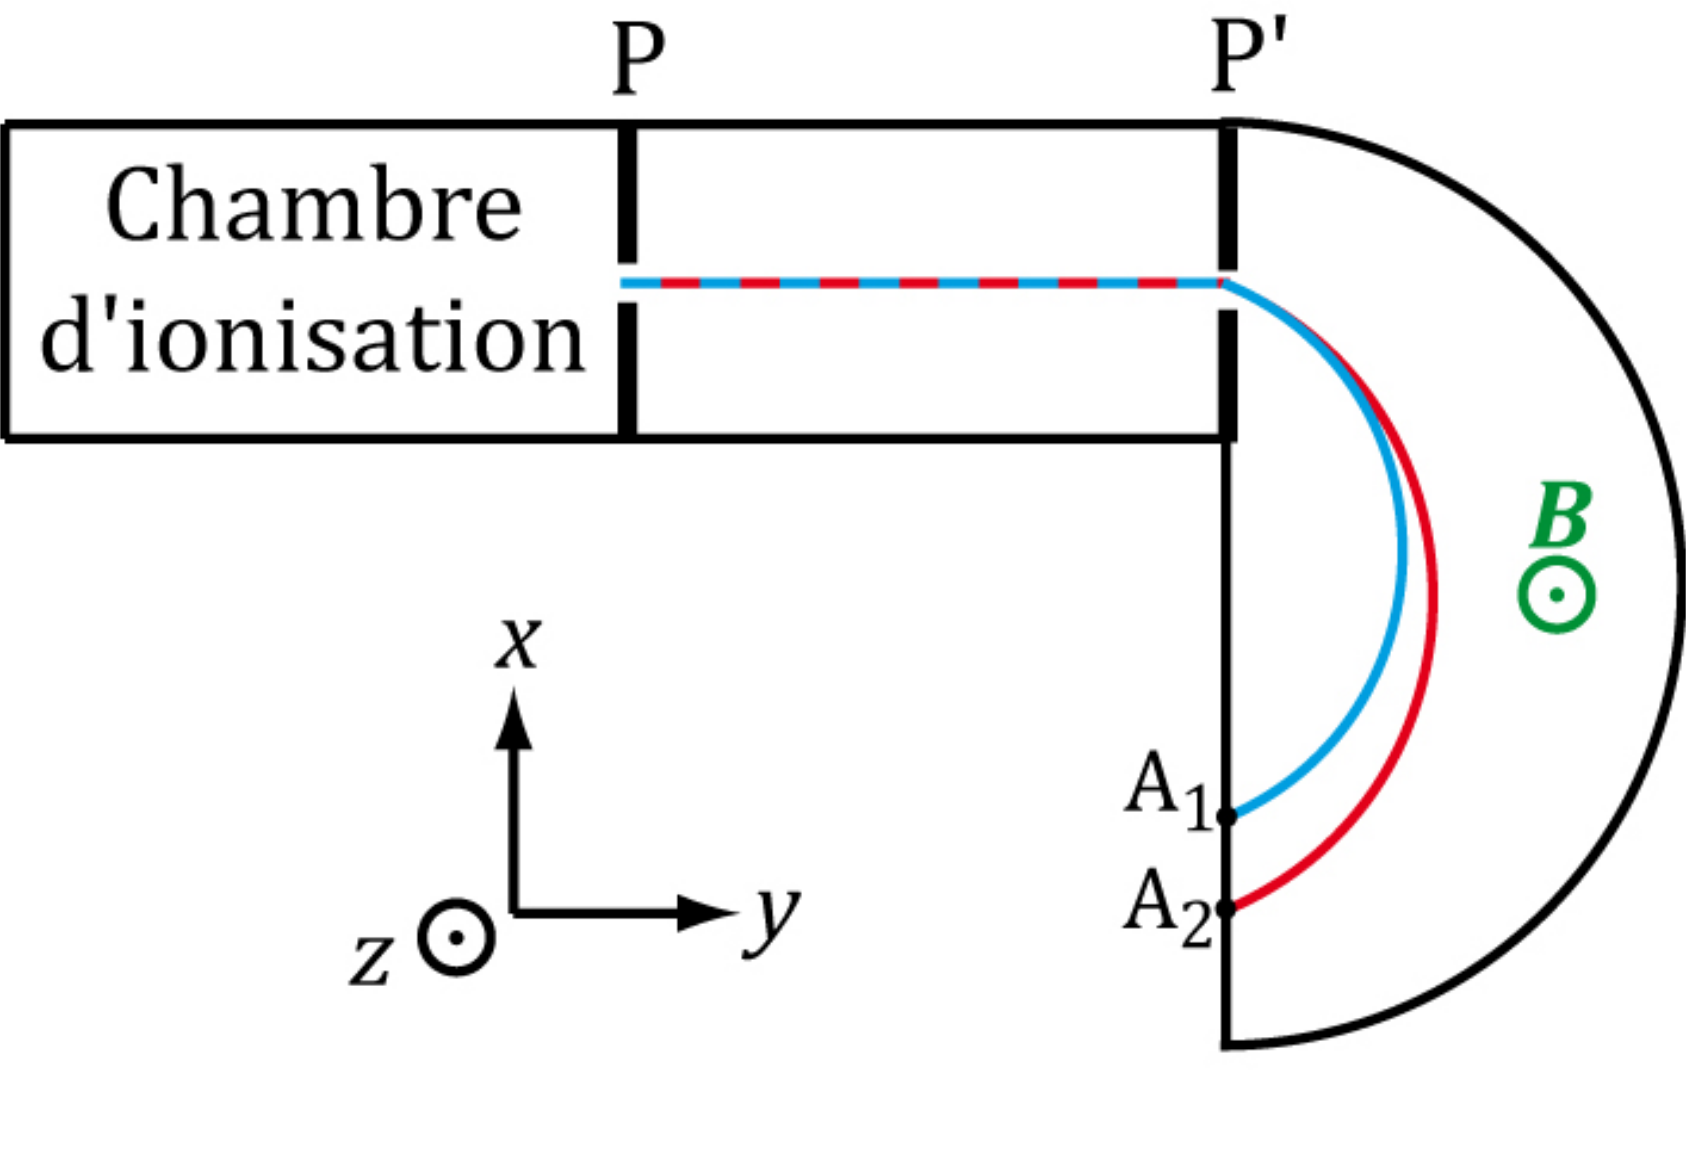
\includegraphics[width=.8\linewidth]{meca/particuleschargees/spectromasse.png}
    \caption{Schéma simplifié d'un spectromètre de masse.}
\end{figure}
\begin{figure}[H]
    \centering
    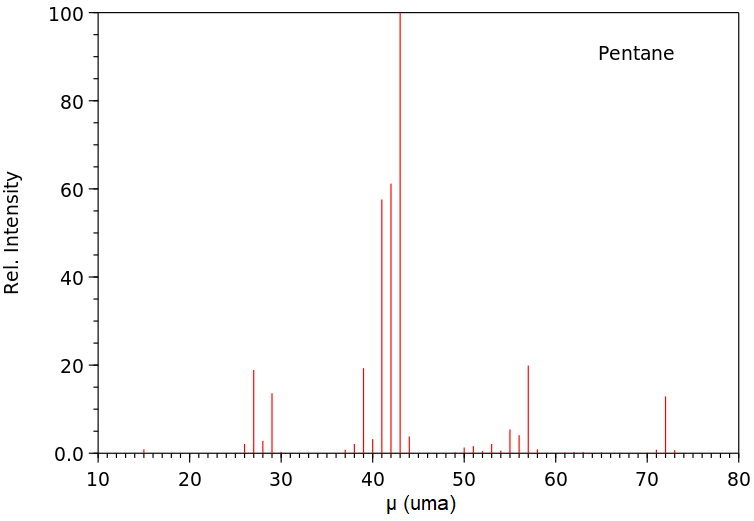
\includegraphics[width=\linewidth]{meca/particuleschargees/mass_pentane.png}
    \caption{Spectre de masse du pentane.}
\end{figure}
\end{multicols}

Le principe est schématisé en figure 1. Dans la chambre d'ionisation on transforme les molécules en ions de faible vitesse. Ils passent ensuite dans un accélérateur linéaire où une tension $U = 8$ kV est imposée entre les plaques $P$ et $P'$. Enfin ils sont soumis dans la zone de déviation à un champ $\vec{B} = B_0\vec{e}_z$, avec $B_0 = 4$ T.

\begin{questions}
    \questioncours Force de Lorentz
    \question On considère deux particules de masse $m_1$ et $m_2$ et de charge $q_1$ et $q_2$. Donner leur vitesse respectives $v_1$ et $v_2$ en sortie de la zone d'accélération. On introduira $\mu = m e/q$, le rapport de masse (sur charge).
    \question Décrire la trajectoire des ions dans la zone de déviation. Quels sont les rayons $R_1$ et $R_2$ de ces trajectoires ?
    \question En déduire l'exrepssion de la distance $d = A_1A_2$ séparant les points d'impact des ions sur la plaque finale en fonction des rapport de masse $\mu_1$ et $\mu_2$. Pourquoi accélère-t-on les ions avant qu'ils entrent dans la zone de déviation ?
    \question Quel est le rapport de masse d'un ion éthyle (chargé +1) dans le SI et en uma ? En ordre de grandeur, calculer la distance nécessaire pour résoudre des écarts de masse de l'ordre d'un nucléon (de 1 uma) sur l'ion méthyle.
    \question On donne le spectre de masse du pentane en figure 2. En quels ions le pentane est susceptible de se fractionner ? Quels sont leur $\mu$ ? Interpréter le spectre.
\end{questions}

\paragraph{Données :}
\begin{itemize}
    \item unité de masse atomique : $1$ uma $= 1,66\times 10^{-27}$ kg ;
    \item masse d'un atome hydrogène : 1 uma, \quad masse d'un atome de carbone : 12 uma ;
    \item charge de l'électron $1,61 \times 10^{-19}$ C.
\end{itemize}
Dans la littérature, $\mu$ est plus souvent noté $m/z$.
\end{exercise}

\begin{solution}
    \begin{questions}
        \questioncours $\vF_\textsc{l} = q\vE + q\vv\wedge\vB$
        \question $\dfrac{1}{2}m v^2 = q U$ donc $v = \sqrt{\dfrac{2Ue}{\mu}}$.
        \question $m\dv{\vv}{t} = q\vv\wedge\vB$ d'ou $\omega_\text{c} = \dfrac{e B_0}{\mu}$ et $R = \dfrac{v \mu}{e B_0} = \sqrt{\dfrac{2U}{e B_0^2}} \sqrt{\mu}$.
        \question $d = \sqrt{\dfrac{2U}{e B_0^2}} (\sqrt{\mu_1} - \sqrt{\mu_2})$.
        \question Ethyle $\mathrm{C_2H_4^+}$ : $m = 28$ uma, $q = e$, $\mu = 28$ uma.
        Donc $d =  \sqrt{\dfrac{2U m_u}{e B_0^2}}(\sqrt{29} - \sqrt{28}) = 130$ $\mu$m.
        \question Typiquement le pentane se fragmente en :
        \begin{align*}
            \mathrm{C_5H_{12}} & \mathrm{\longrightarrow C_5H_{12}^+ \text{\small ($\mu = 72$)} + e^-} \\
            \mathrm{C_5H_{12}} & \mathrm{\longrightarrow C_4H_9^+ \text{\small ($\mu = 57$)} + CH_3^\bullet + e^-} \\
            \mathrm{C_5H_{12}} & \mathrm{\longrightarrow C_3H_7^+ \text{\small ($\mu = 43$)} + C_2H_5^\bullet + e^-} \\
            \mathrm{C_5H_{12}} & \mathrm{\longrightarrow C_2H_5^+ \text{\small ($\mu = 29$)} + C_3H_7^\bullet + e^-} \\
            \mathrm{C_5H_{12}} & \mathrm{\longrightarrow CH_3^+ + \text{\small ($\mu = 15$, non résolu)} + C_4H_9^\bullet + e^-}
        \end{align*}
        Les petits pics off de 1 ou 2 par rapport aux grands sont liés à des pertes d'un H typiquement.
    \end{questions}
\end{solution}
\begin{exercise}{Mouvement cyclotron avec dérive électrique}{2}{Sup}
{Particules chargees}{bermudez}

On s'intéresse au mouvement d'un électron dans un faisceau électronique cylindrique soumis à un champ magnétique $\vB = B_0\ve_z$.

\begin{questions}
    \questioncours Mouvement cyclotron. On fera la démonstration de la loi horaire du mouvement et on donnera l'expression de la pulsation cyclotron $\omega_c$.
    \uplevel{\`A cause du faisceau électronique, l'électron est également soumis à un champ électrique
    $$\vE = -\dfrac{n e}{2\ep_0} \vr,$$
    $n$ étant la densité (par m$^3$) d'électrons.}
    \question Écrire la nouvelle expression de la Force de Lorentz. \`A quelle force mécanique le terme électrique vous fait-il penser ?
    \question Établir les équations du mouvement de la particule pour $x(t)$ et $y(t)$. On considérera que la particule n'a pas de mouvement suivant $z$.
    \question Introduire la pulsation cyclotron $\omega_c$ ainsi qu'une autre puslation caractéristique, notée $\omega_p$, la pulsation plasma, pour simplifier l'expression précédente.
    \question On introduit $\cal{Z}(t) = x(t) + i y(t)$. Donner l'équation temporelle vérifiée par $\cal{Z}(t)$.
    \question Résoudre l'équation sous forme complexe et donner une condition sur $\dfrac{\omega_c}{\omega_p}$ afin que le mouvement soit borné.
    \question Pour finir, donner la loi horaire $\cal{Z}(t)$ et caractériser le mouvement.
\end{questions}

\end{exercise}

\begin{solution}
    \begin{questions}
        \questioncours $\omega_\text{c} = \dfrac{eB_0}{m}$.
        \question Le terme électrique est une force centrale (répulsive car $q = -e$) : $\vF_\textsc{l} = q\vE + q\vv\wedge\vB = -\dfrac{nqe}{2\ep_0}(x\ve_x + y\ve_y) + q B (\dot{y}\ve_x - \dot{x}\ve_y)$
        \question \begin{align*}
            \ddot{x} &= \omega_p^2x - \omega_c \dot{y} \\
            \ddot{y} &= \omega_p^2y + \omega_c \dot{x}
        \end{align*}
        \question avec $\omega_p = \dfrac{nq^2}{m\ep_0}$.
        \question $\ddot{\cal{Z}} = \omega_p^2\cal{Z} -i\omega_c\dot{\cal{Z}}$.
        \question Si $\cal{Z} = e^{i\omega t}$ :
        $$\omega^2 + \omega_p^2 - \omega \omega_c = 0.$$

        On a donc $\omega = \dfrac{\omega_c}{2}\qty(1 \pm \sqrt{1-4\omega_p^2/\omega_c^2})$. Il faut $\omega_p < \omega_c/2$ pour avoir $\omega$ imaginaire pur.
        \question Donc $\cal{Z} = A e^{i\omega_+ t} + B e^{i\omega_- t}$ : c'est la combinaison de deux mouvements circulaires, soit une épicycle. Si $\omega_p = 0$ on retrouve un mouvement circulaire à la pulsation $\omega_c$. Si $\omega_p = \omega_c/2$ (cas limite), on trouve $\omega_{\pm} = \frac{\omega_c}{2}$ : Le mouvement est aussi circulaire, mais deux fois plus lent.
    \end{questions}
\end{solution}
\begin{exercise}{Mouvement cyclotron avec dérive magnétique}{2}{Sup}
{Particules chargees}{bermudez}

On s'intéresse au mouvement d'une particule chargée dans un champ magnétique.

\begin{questions}
    \questioncours Mouvement cyclotron. On fera la démonstration de la loi horaire du mouvement et on donnera l'expression de la pulsation cyclotron.
    \uplevel{Dans la vie réelle, les champs magnétiques uniformes+ n'existent pas... Typiquement, pour avoir des dispositifs type cyclotron, on a un champ dans une direction fixe, axisymétrique, qui est maximal sur cet axe et nul loin de l'axe. On modélise la situation comme suit, en géométrie cylindrique, $\vB = B(r) \ve_z$.}
    \question Donner une fonction $B$ qui telle qu'elle décroît continûment de $B(r=0) = B_0$ à $B(r\rightarrow +\infty)= 0$.
    \question \'Etablir les équations du mouvement de la particule. Ces équations peuvent-elles être résolues comme précédemment ?
    \question La force de Lorrentz magnétique travaille-t-elle ? Par conséquent, donner une grandeur $V$, homogène à une vitesse, qui est conservée lors du mouvement. Justifier qu'on puisse considérer qu'il n'y a pas de mouvement suivant $z$.
    \question On introduit une autre grandeur $w =r\dot{\theta} + g(r)$. Que doit valoir $g(r)$ afin que $w$ soit également une constante du mouvement ? On prendra $w(r=0) = 0$.
    \question À l'aide des deux questions précédentes, donner l'expression de $\dot{r}^2$ en fonction de $r$ uniquement, et des deux constantes du mouvement $V$ et $w$.
    \question Montrer que le mouvement de la particule est borné.
    \question Déduire que tout se passe comme si on avait une particule de masse $m$ dans un potentiel $V(r)$.
\end{questions}

\end{exercise}

\begin{solution}
    \begin{questions}
        \questioncours $\omega_\text{c} = \dfrac{eB}{m}$.
        \question Exemples : $B(r) = B_0 e^{-r/\lambda}$, $B(r) = B_0 e^{-r^2/2\lambda^2}$, $B(r) = \dfrac{B_0}{1+(r/\lambda)^2}$... \`A ce niveau, prendre une fonction qui s'intègre bien (pas la gaussienne).
        \question \begin{align*}
            \ddot{r} - r \dot{\theta}^2 &= \omega_c \dot{\theta} r b(r) \\
            r\ddot{\theta} + \dot{r}\dot{\theta} &= -\omega_c \dot{r} b(r) \\
            \ddot{z} &= 0
        \end{align*}
        \question Travail nul donc énergie cinétique conservée donc $V^2 = \dot{r}^2 + r^2\dot{\theta}^2$ conservée. ($\dot{z}$ étant également un invariant mais on n'a pas besoin de se le trainer).
        \question $\dv{t} \qty\Big(r\dot{\theta} + g(r)) = \dot{r}\qty\Big( -\omega_c b(r) + g'(r))$ donc on prend $g(r) = \omega_c \int_0^r b(\rho)\dd{\rho}$. $w = r\dot{\theta} + g(r)$ est ainsi conservée.
        \question Ainsi,
        $$\dot{r}^2 = V^2 - (w - g(r))^2.$$
        \question
        Et donc  $\abs{w - g(r)} < V$
        \question On dérive la Q6 :
        $$\ddot{r} = g'(r)\times(w-g(r))$$
        On retrouve la considération précédente (comme $g'(r)>0$).
    \end{questions}
\end{solution}

\section{Mécanique du solide}
\begin{exercise}{Vitesse d'un satellite sur son orbite elliptique}{2}{Sup}
{Mécanique, Moment cinétique}{correge}

On considère un satellite de masse 1 tonne en orbite elliptique autour de la Terre. Le satellite se maintient sur cette trajectoire car il est soumis à la force gravitationnelle qu’exerce sur lui la Terre. Cette force est en permanence dirigée vers le centre de la Terre. On note :
\begin{itemize}
    \item $O$ le centre de la Terre qui est un des foyers de l’ellipse;
    \item $C$ le centre de l’ellipse;
    \item $A$ l’apogée du satellite (point de l’orbite le plus éloignée de la surface de la Terre);
    \item $P$ son périgée (point de l’orbite le plus proche de la surface de la Terre);
    \item $A'$ le point de la surface de la Terre qui fait face à A, l’apogée du satellite;
    \item $P'$ le point de la surface de la Terre qui fait face à P, le périgée du satellite;
    \item $S$ le point tel que $\vec{CS}$, vertical dirigé vers le haut, représente le demi-petit axe de l’ellipse.
\end{itemize}
On donne les grandeurs suivantes :
\begin{itemize}
    \item Distance $CS=16715$km;
    \item Distance $AA'=35000$km;
    \item Distance $PP'=350$km;
    \item Distance $OA'=OP'=RT=6400$km;
\end{itemize}
On considère que le satellite est en mouvement dans un référentiel galiléen dont le centre est situé au centre de la Terre.

\begin{questions}
    \questioncours Moment cinétique.
    \question Réaliser une figure comportant toutes les indications de l’énoncé. Représenter le satellite en $S$ avec sa vitesse $\vec v$ et les vecteurs polaires unitaires.
    \question La vitesse en $S$ est $v_S=\SI{14650}{km.h^{-1}}$. Calculer le moment cinétique du satellite en $S $ par rapport au point $O$ (un angle permettant de repérer le satellite peut être utile).
    \question En appliquant le théorème du moment cinétique, trouver la vitesse du satellite à son apogée $A$ et à son périgée $P$.
\end{questions}

\end{exercise}

\begin{solution}
\begin{questions}
    \questioncours 
    \question 
    \question $L_O(S)=mvCS=\SI{2.4e17}{kg.m^2.s^{-1}}$
    \question Avec le théorème du moment cinétique, on trouve un moment cinétique est constant. On sait qu'au périgée et à l'apogée, rayon vecteur et vitesse sont orthogonales. Donc $v_A=\SI{5.9e3}{km.h^{-1}}$, $v_P=\SI{3.6e4}{km.h^{-1}}$
\end{questions}

\end{solution}


\begin{exercise}{Pendule simple incliné}{2}{Sup}
{Mécanique, Moment cinétique}{correge}

On réalise un pendule simple à l’aide d’un mobile autoporteur sur table à coussin d’air. Le mobile de masse $m$ est accroché à l’extrémité d’un fil de longueur $\ell$ dont l’autre extrémité est attachée à un point fixe $O$ de la table.Le mobile peut alors se déplacer sans frottement dans un plan $xOy$.

\begin{center}
    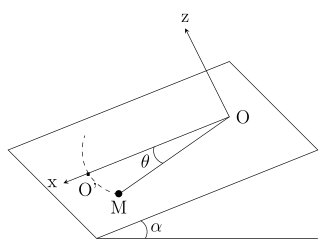
\includegraphics[scale=0.6]{meca/mecasolides/pendule_incline}
\end{center}

\begin{questions}
    \questioncours Moment cinétique.
    \question Exprimer le moment cinétique de $M$ par rapport à $O$.
    \question Identifier les forces et exprimer leur projection sur la base cylindrique.
    \question Appliquer le théorème du moment cinétique afin d’établir l’équation différentielle du mouvement dans le cas des petites oscillations.
    \question En déduire l’expression de la période des petites oscillations.
    \question Le pendule est lancé depuis sa position d’équilibre $O$’ avec un vitesse initiale $v_0$. Quel est l’angle maximal atteint (l’hypothèse des petites oscillations étant toujours valable) ?
\end{questions}

\end{exercise}

\begin{solution}
\begin{questions}
    \questioncours 
    \question $L = m\ell^2 \dot{\theta}^2$
    \question $\vec{P} = mg(\sin \alpha \cos \theta, -\sin \alpha \sin \theta,  -\cos \alpha)_{(r,\theta,z)}$
    \question $\ddot \theta + \theta \frac{g}{\ell}\sin \alpha = 0$
    \question $\omega_0^2 = \frac{g}{\ell}\sin \alpha$
    \question On trouve la solution, et on cherche le maximum. On trouve $\theta_{max} = \frac{v_0}{\ell \omega_0}$
\end{questions}

\end{solution}


%\begin{exercise}{La poutre}{2}{Sup}
{Mécanique,Moment cinétique, Couple}{lelay}

On considère une poutre de longueur $L$ et de masse $M$, qui est portée à l'horizontale par deux bûcherons. L'un d'eux se trouve à l'une des extrémités de la poutre, l'autre se trouve à une distance $\ell$ du premier. Les bûcherons ne peuvent exercer sur la poutre que des forces dirigées verticalement.

\begin{questions}
    \questioncours Moment d'une force en un point.
    \question Sans calculs, quel est la force exercée par chacun des bûcherons sur la poutre dans le cas (a) $\ell = L$ et $\ell = L/2$ ?
    \question Montrer que l'équilibre de la poutre en position horizontale se traduit par un système de deux équations.
    \question Tracer la force exercée par chaque bûcheron pour la maintenir position horizontale en fonction de $\ell$. Que se passe-t-il pour $\ell \rightarrow 0$ ?
    \question Le bûcheron situé à l'extrémité de la poutre se suspend à elle pour faire une farce à son collègue. Quel est le poids que celui-çi doit alors soulever ? Où doit-il se placer sur la poutre ?
\end{questions}

\end{exercise}

\begin{solution}
    \begin{questions}
    \questioncours $M = OP x F$
    \question $\ell = L$ : chacun soulève un poids $M/2$. $\ell = L/2$ : le bucheron au centre soulève toute la poutre, l'autre ne sert à rien.
    \question Équilibre des forces (PFD sur la poutre) : $F_1 + F_2 = Mg$. Équilibre des moments (TMC sur la poutre) $F_1 \frac{L}{2} + F_2 \qty(\frac{L}{2}-\ell)$
    \question $F_2 = Mg\frac{L}{2\ell}$ ; $F_1 = Mg\qty(1 - \frac{L}{2\ell})$
    \question En notant $m$ la masse du bûcheron farceur, $F_1 = -mg$ et donc $F_2 = (M+m)g = Mg\frac{L}{2\ell}$ d'où $\ell = \frac{L}{2}\frac{M}{M+m}$. On a bien $\ell < L/2$ puisque $F_1 < 0$
    \end{questions}
\end{solution}
% Niveau :      PCSI *
% Discipline :  Méca
% Mots clés :   Ballistique, Mécanique du point, PFD, Chute libre

\begin{exercise}{Le bûcheron canadien}{2}{Sup, Spé}
{Mécanique,Moment cinétique}{bermu}

Un bûcheron canadien veut abattre un pin qui est légèrement incliné suite à une tempête. On assimile cet arbre à une tige longue et homogène de longueur $L$ et de masse $m$. Alors qu'il scie l'arbre à la base du tronc, l'arbre se met à tomber s'appuyant sur la base de la souche, supposée fixe lors de la chute.

On appelle $\theta$ l'inclinaison de l'arbre par rapport à la verticale.

\begin{questions}
    \question \'Etablir l'équation du mouvement de l'arbre lors de sa chute.
    \question Montrer que la vitesse de chute de l'arbre peut s'écrire
    $$\dot{\theta} = \dfrac{1}{\tau}\sqrt{\cos\theta_0 - \cos\theta},$$
    $\tau$ étant un temps caractéristique dont on déterminera l'expression.
    \question En déduire le temps de chute de cet arbre à l'aide de $\tau$ et de la fonction
    $$I(\theta_0) = \int_{\theta_0}^{\pi/2}\dfrac{\dd{\theta}}{\sqrt{\cos\theta_0 - \cos\theta}}.$$
    Quel est le temps du chute pour un arbre de 20m initialement incliné à $5^\circ$ ? Le bûcheron aura-t-il le temps de reculer ?
\end{questions}

\plusloin
Que cela changerait-il si le tronc glissait sur le sol lors de sa chute ? S'il tournait sur sa base ?

\paragraph{Données :}
\begin{itemize}
    \item Le moment d'inertie d'un cylindre fin $J = \frac{1}{3}mL^2$,
    \item Graphe de la fonction $I(\theta_0)$ :
        \begin{figure}[H]
            \centering
            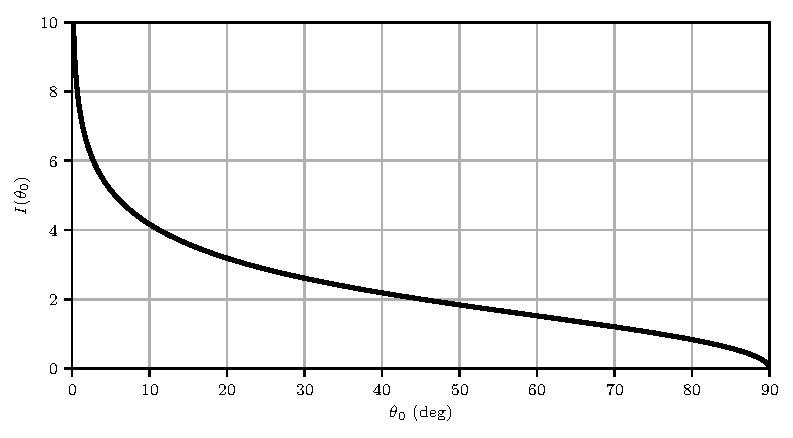
\includegraphics[scale=1]{meca/fonction_I.pdf}
            \vspace{-1em}
            \caption{Graphe de la fonction $I(\theta_0)$.}
        \end{figure}
\end{itemize}

$$\text{En }\theta_0 \rightarrow 0^+, \qquad I(\theta_0) \simeq - \sqrt{2}\ln(\theta_0/\pi).$$
\end{exercise}
% Niveau :      PCSI
% Discipline :  Méca

\begin{exercise}{Le crayon immobile}{3}{Sup, spé}
{Mécanique,Moment cinétique,Mécanique quantique}{lelay}

On considère un crayon de papier extrêmement bien taillé, au point que sa pointe ne soit plus épaisse que d'un atome à son bout. On essaye de le poser sur la pointe de manière à ce qu'il reste vertical le plus longtemps possible. 
On appelle $\theta$ l'inclinaison du crayon par rapport à la verticale et $J$ son moment d'inertie par rapport au point où est posée la pointe, supposé immobile.

\begin{questions}
    \question Modéliser la situation, faire un schéma.
    \question \'Etablir l'équation du mouvement de du crayon lors de sa chute.
    \question On s'intéresse au mouvement initial. Réécrire l'équation précédente dans la limite des petits angles. Cette équation est-elle stable en $\theta = 0$ ?
    \question Donner une estimation numérique du temps caractéristique de chute du crayon $\tau$.
    \question Résoudre l'équation précédente pour un angle initial $\theta_0$ et un moment angulaire initial $L_0 = \frac{J}{\tau} \theta_0$. Quelle est la condition nécessaire pour que le crayon reste vertical ? Pensez-vous que ce soit (en théorie du moins) réalisable ?
    \question En réalité, la relation d'indétermination de Heinsenberg impose $\theta_0 L_0 \geq \frac{\hbar}2$. Quel est alors le $\theta_0$ minimal atteignable ?
    \question Exprimer $t_1$, le temps auquel $\theta = \theta_1$ radians, en fonction de $\tau$ et de $\theta_0$. 
    \question Le temps de chute du crayon entre $\theta_1$ et $\frac\pi2$ est $t_2 = \tau \: I(\theta_1)$ où $I$ est une fonction que l'on ne cherchera pas à exprimer. \\
    Donner le temps maximal de chute d'un crayon. Ce résultat vous semble-t-il étonnant ?
\end{questions}

\plusloin
Retrouver l'expression de la fonction $I$ sous forme d'une intégrale.

\paragraph{Donnée :}~\vspace{-3em}\\
\begin{figure}[H]
    \centering
    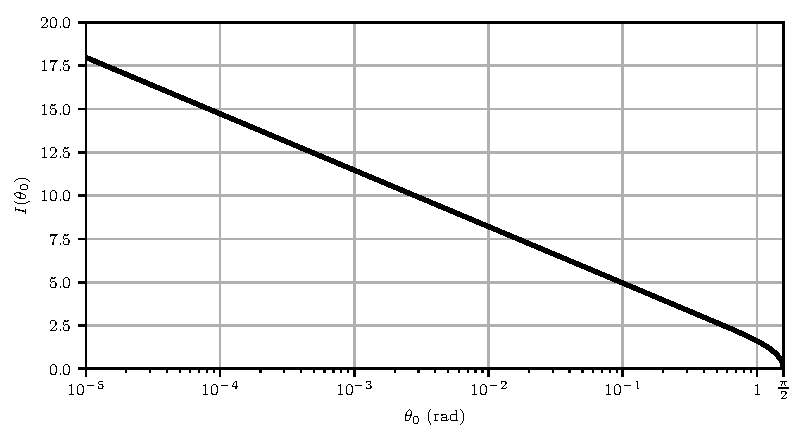
\includegraphics[scale=1]{meca/fonction_Ilog.pdf}
    \vspace{-1em}
    \caption{Graphe de la fonction $I(\theta_0)$.}
    \end{figure}
\end{exercise}
%% Niveau :      sup
% Discipline :  Méca

\begin{exercise}{Fluctuation de la durée du jour}{3}{Sup, spé}
{Mécanique,Moment cinétique}{bermudez}


\begin{questions}
    \questioncours Présenter l'analogie entre moment cinétique et quantité de mouvement, et discuter de leur conservation. On fera un tableau pour comparer les différentes grandeurs en jeu dans chaque cas.
    \uplevel{
La durée du jour, $\tau_\text{j}$, actuellement de 24h, fluctue sur des échelles de temps très variées allant de quelques jours sur plusieurs millions d'années. La figure ci-dessous représente la variation de la durée d'une journée depuis les années 1900.

\begin{figure}[H]
    \centering
    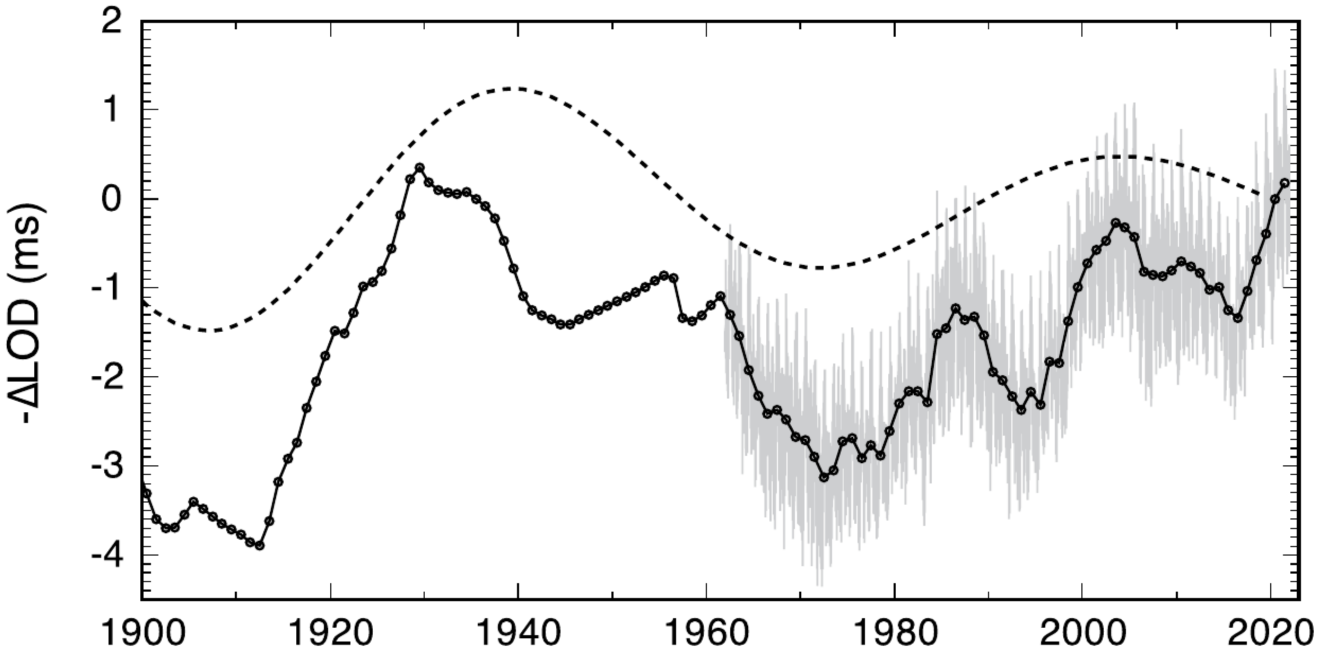
\includegraphics[width=.7\linewidth]{meca/mecasolides/lengthoftheday.png}
    \caption{Variation de la durée d'une journée en millisecondes par rapport aux 24h standard.}
    \label{fig:LOD}
\end{figure}

Il y a plusieurs million d'années, elle était de 22h. Par l'effet du couplage Terre--Lune, elle a augmentée graduellement avec le temps.

Il a été mis en évidence très récemment, que la durée du jour pouvait également fluctuer sur des périodes d'environ 70 ans (en pontillés sur la figure~\ref{fig:LOD}) à cause du renversement de la rotation du noyau interne de la Terre, qui libre de tourner dans le noyau externe, liquide, est presque immobile depuis 2013.

La durée du jour fluctue également sur des échelles de temps plus courtes par couplage entre l'atmosphère et la Terre. Pour des échelles de temps de l'ordre de quelques jours à quelques années (en gris sur la figure~\ref{fig:LOD}), cela est principalement attribué aux courants atmosphériques globaux, comme les alizés (vents d'est, à l'équateur en basse altitude), les vents d'ouest (latitude $30^\circ$, basse altitude) et les jet stream (vents d'ouest aux latitudes $60^\circ$ en haute altitude), qui ont des vitesses qui varient sur des valeurs de l'ordre de 100 km/h typiquement.

\textsf{Problème ouvert :} en utilisant les résultats de la question précédente et à l'aide des données, estimer en ordre de grandeur les quantités suivantes :
}

    \question la fluctuation d'une journée due à l'arrêt de la rotation du noyau interne de la Terre ;
    \question la fluctuation d'une journée due aux courants atmosphériques globaux ;
    \question l'éloignement moyen entre la Terre et la Lune en cm/siècle.
\end{questions}

\paragraph{Données :}(toutes ne sont pas utiles)\\[-2em]
\begin{multicols}{2}
\begin{itemize}
    \item masse de la Terre : $m_\textsc{t} = 6,0\times 10^{24}$ kg ;
    \item masse de la Lune : $m_\textsc{l} = 7,4\times 10^{22}$ kg ;
    \item masse de l'atmosphère : $m_\text{a} = 5,3\times 10^{18}$ kg ;
    \item densité normale de l'air au niveau de la mer : $\rho = 1,3\ \mathrm{kg\cdot m^{-3}}$ ;
    \item densité myenne du noyau interne : $\rho = \SI{12 300}{kg/m3}$ ;
    \item distance Terre--Lune : 384 400 km ;
    \item rayon moyen de la Terre : $R_\textsc{t} = 6371$~km ; 
    \item rayon moyen du noyau interne : $R_\text{n} = 1220$~km ;
    \item constante universelle de gravitation : $G = 6,67\times 10^{-11}$ SI ;
    \item moment d'inertie d'une boule remplie uniformément : $J=\dfrac{2}{5}MR^2$ ;
    \item moment d'inertie d'une sphère creuse : $J=\dfrac{2}{3}MR^2$ ;
    \item moment d'inertie d'un anneau fin : $J =MR^2$.
    \item
\end{itemize}
\end{multicols}
\end{exercise}

\begin{solution}

\plusloin~\\[-2em]
\begin{itemize}
    \item Retrouver la masse de l'atmosphère et de la Terre à partir des données ;
    \item Retrouver les formules littérales des moments d'inertie ;
\end{itemize}

\end{solution}

\section{Mécanique céleste}
% Niveau :      PCSI
% Discipline :  Mécanique céleste
%Mots clés :    Astronaute

\begin{exercise}{Autour des vitesses cosmiques}{1}{Sup}
{Mécanique, Mécanique céleste}{lelay}


\begin{questions}
    \questioncours Donnez la définition de la vitesse d'échappement. Quelle est celle de la Terre ?
    \question Quelle est la distance des satellites géostationnaires par rapport à la Terre ? Quelle est leur vitesse de déplacement ?
    \question Un cosmonaute échoué sur un astéroïde de rayon $R$ et de même densité que la terre parvient a s’en échapper en sautant. Quelle est la valeur maximale de $R$ ?
\end{questions}

\end{exercise}

\begin{solution}

\begin{questions}
    \questioncours $\frac12 m v ^2 - GMm/R = 0 \Rightarrow v =\sqrt{2GM/R} \approx 11$ km/s
    
    \question 3e loi de Kepler $R^3/T^2 = GM/4\pi^2$ d'où avec $T = $24 h, $R = 42300$ km. Vitesse $v = R\omega = 2\pi R/T = \sqrt{GM/R}$ soit 3 km/s.
    
    \question Il faut prendre comme vitesse d'échappement la vitesse maximale d'un être humain (autour de 10 m/s pour les champions olympiques) et en déduire $R$, en sachant que $M = \frac43 \pi \rho_T R^3 = M_T R^3/{R_T}^3$ selon que l'élève connaisse mieux la masse de la Terre ($6\times 10^{24}$ kg) ou sa densité ($5000$ kg/m$^3$). On trouve en OdG 10 km.
\end{questions}

\end{solution}

% Niveau :      PC *
% Discipline :  Méca
% Mots clés :   Lune

\begin{exercise}{Autour des trous noirs}{2}{Sup, Spé}
{Mécanique,Mécanique céleste}{bermu}

\begin{questions}
    \questioncours Vitesse de satellisation (\emph{i.e.} la vitesse nécessaire à un corps pour échapper à la gravité de l'astre sur lequel il se trouve).
    \question Définir brièvement ce qu'est un trou noir (et éventuellement l'horizon des évènements) et comment il se forme.
\begin{EnvUplevel}
Pour un trou noir classique, on peut estimer quelle est la taille critique $R_\textsc{s}$ en dessous de laquelle un objet de masse $M$ devient un trou noir en disant qualitativement que "même la lumière ne peut pas échapper à la gravité du trou noir".
\end{EnvUplevel}
    \question En utilisant les résultats de la question de cours, explicitez sous forme de formule mathématique la phrase précédente.
    \question En déduire le rayon de Schwarzschild $R_\textsc{s}$, en fonction de la masse de l'objet $M$ ainsi que du rayon $R_\odot$ et de la masse $M_\odot$ du soleil. Ce résultat est malgré toutes nos approximations exact !\\
    De combien doit-on réduire la taille du soleil pour qu'il devienne un trou noir. Interpréter au regard de la question 2.
\uplevel{\plusloin ~\vspace{-1em}}
    \question Discuter qualitativement des limites du modèle. Interpréter le terme de \emph{lentille gravitationelle}
\begin{EnvUplevel}
Dans le cas où le trou noir est en rotation à la vitesse $\Omega$ (trou noir de Kerr), comme par exemple le système binaire \textsf{GRS 1915+105}, l'horizon des évènements est donné par la relation
$$R_\textsc{k} = \dfrac{R_\textsc{s}}{2}\qty[1 + \sqrt{1 - \qty(\dfrac{2}{5}\dfrac{R^2 \Omega}{R_\textsc{s}\:c})^2}].$$
\end{EnvUplevel}
    \question Interpréter cette équation. Quid du soleil et de la terre ?
\end{questions}

\paragraph{Données :}
\begin{itemize}
    \item constante universelle de gravitation $G = \SI{6,674e-11}{SI}$,
    \item vitesse de la lumière dans le vide $c = \SI{2,998e8}{m.s^{-1}}$,
    \item masse du soleil $M_\odot = \SI{1,989e30}{kg}$,
    \item rayon du soleil $R_\odot = \SI{6,963e8}{m}$.
    \item période de rotation du soleil $T_\odot = 27$ j.
\end{itemize}
\end{exercise}

\begin{solution}  
    \begin{questions}
        \question $\En_p = \En_c$
    \end{questions}
\end{solution}
% Niveau :      PCSI - PC
% Discipline :  Méca
% Mots clés :   Hohmann

\begin{exercise}{Orbite de Hohmann}{2}{Sup,Spé}
{Mécanique,Mécanique céleste}{lelay}

On cherche à mettre un satellite en orbite géostationnaire. Dans un premier temps, on le met en orbite circulaire autour de la Terre à une altitude de 300 km au dessus du sol.

\begin{questions}
    \questioncours Donner l'expression et la valeur altitude d'un satellite géostationnaire.
    \question Donner l'énergie mécanique d'un satellite en orbite stationnaire à un rayon $R$ autour de la Terre en fonction de $R$ et d'une constante $K$ que l'on précisera. En déduire par analogie l'énergie de ce satellite sur une orbite elliptique de demi grand axe $a$.
    \question En repartant de la formule générale de l'énergie mécanique, donner la vitesse $v$ d'un mobile de masse $m$ en orbite elliptique autour de la Terre en fonction de $r$, $a$ et de $K$.
    \question On veut passer d'une orbite circulaire de rayon $R_-$ à une orbite circulaire de rayon $R_+$ en utilisant une \textit{orbite de transfert} elliptique, de manière à utiliser le moins de carburant possible (minimiser les phases d'accélération). Faire un schéma et proposer une telle orbite.
    \question Donner la quantité totale d'énergie cinétique à fournir en tout. Montrer qu'elle est minimale.
    \question Expliquer pourquoi cette technique est utilisée pour les voyages visant à rejoindre l'ISS.
\end{questions}
\end{exercise}

\begin{solution}

\begin{questions}
    \questioncours 3e loi de Kepler $R^3/T^2 = GM/4\pi^2$ d'où avec $T = $24 h, $R = 42300$ km, d'où une \textbf{altitude} d'environ 36000 km.
    \question On a (3e loi de Kepler) $R^3\omega^2 = GM$ or $v = R\omega$ soit $v = \sqrt{GM/R} = \sqrt{K/R}$ avec $K = GM$. D'où l'énergie mécanique $E = \frac12 m v^2 - \frac{mMG}{R} = \frac12 \frac{Km}{R} - \frac{Km}{R} = -\frac12\frac{Km}{R}$ on retrouve le résultat bien connu. On généralise pour une ellipse en remplaçant $R$ par $a$ : $E = -\frac12\frac{Km}{a}$
    \question On a $E = \frac12m v^2 - \frac{Km}{r}$ soit $v^2 = -\frac{K}{a} - \qty(-\frac{K}{2r})$ d'où $v = \sqrt{K}\sqrt{\frac2r-\frac1a}$
    \question Il faut en gros proposer le schéma suivant :
    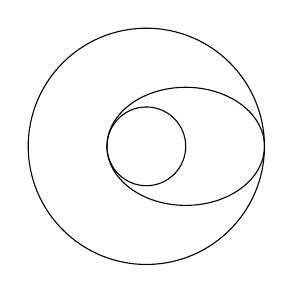
\begin{tikzpicture}
    
    \draw (0,0) ellipse (0.5);
    \draw (0.5,0) ellipse (1 and 0.75);
    \draw (0,0) ellipse (1.5);
    
    \end{tikzpicture}
    La petite orbite est l'orbite initiale, la grande l'orbite finale, et entre les deux une orbite qui interpole.
    Il y a donc 3 étapes, et pour passer de chaque orbite a la suivante on met un coup d'accélérateur, i.e. on change de vitesse.
    Le demi grand axe de l'orbite de Hohmann est évidemment $a = (R_- + R_+)/2$.
    \question 
    \begin{itemize}
        \item Transition départ -> Hohmann : la vitesse passe de $v = \sqrt{\frac{K}{R_-}}$ à $v' = \sqrt{K}\sqrt{\frac{2}{R_-}-\frac1a}$ d'où $\Delta {E_c}_1 = \frac1{2} m ({v'}^2 - v^2) = \frac{12}mK\qty(\frac{1}{R_-} - \frac1a)$
        \item Transition Hohmann -> arrivée : la vitesse passe de $v = \sqrt{K}\sqrt{\frac{2}{R_+}-\frac1a}$ à $v' = \sqrt{\frac{K}{R_+}}$ d'où $\Delta {E_c}_2 = \frac1{2} m ({v'}^2 - v^2) = \frac{12}mK\qty(\frac{1}{a} - \frac1{R_+})$
    \end{itemize}
    Au total on a donc dépensé une énergie $\Delta {E_c}_1 + \Delta {E_c}_2 = \frac{12}mK\qty(\frac{1}{R_-} - \frac1{R_+}) = {E_m}_\text{finale} - {E_m}_\text{initiale}$ : aucune dépense superflue.
    \question C'est la moins coûteuse en énergie puisqu'elle est optimale. En pratique on utilise plusieurs orbites de transfert, en diminuant l'ellipticité quand on s'approche de la cible (3 orbites pour l'ISS).
\end{questions}

Masse de la Terre : $6\cdot 10^{24}$ kg

Rayon de la Terre : 6400 km
\end{solution}
\begin{exercise}{Points de Lagrange}{3}{Sup, Spé}
{Mécanique,Mécanique céleste,Mécanique en référentiel non galiléen}{lelay}

\begin{questions}
    \questioncours Position d'équilibre d'un satellite dans un champ gravitationnel et lois de Kepler.
\uplevel{Nous nous plaçons désormais dans le référentiel héliocentrique $(S ; r,\theta)$ en coordonnées polaires dans lequel la Terre $T$ est fixe en $r = R_\oplus = 1$ U.A. et $\theta=0$.}
\question Ce référentiel est-il Galiléen ?
\begin{EnvUplevel}
Dans ce cas, pour un corps de masse $m$, il faut prendre en compte la force centrifuge d'inertie
$$\vf_i = m\omega^2\vr,$$
dans le bilan des forces, avec $\omega$ la période orbitale de la Terre.
\end{EnvUplevel}
    \question Quelle est la valeur de $\omega$ ? Donner l'expression de $\omega$ à l'aide de la troisième loi de Kepler.
\uplevel{On appelle points de Lagrange, les positions d'équilibre d'un satellite de la terre dans le précédent référentiel.}
    \questionbonus Contributions scientifiques de Joseph-Louis Lagrange.
    \question Donnez l'équation vectorielle de ce point $\vr$ sans chercher à la résoudre pour le moment. \\
    Exprimer cette équation uniquement en fonction de
    $$Q = \dfrac{M_\oplus}{M_\odot} \qqtext{et} \vu = \dfrac{\vr}{R_\oplus}.$$
    \question Cette équation n'étant pas très simple, nous allons chercher plusieurs solutions particulières :
    \begin{parts}
        \part En projetant l'équation sur l'axe $\ve_y$, montrez que l'équation admet que le point de Lagrange se situe sur l'axe Terre--Lune. \\
        Nous ne regardons pas le second cas.
        \part Chercher les solutions de cette équation dans l'axe Terre -- Lune, proche de la Terre \emph{i.e.} $u \simeq 1$. \\
        Discuter de la pertinence de cette approximation.
        \part Comparer avec la position de la Lune ou d'un satellite en orbite géostationnaire et commenter.
        \part (\emph{Question facultative}) Ou chercheriez vous d'autres solutions sur l'axe des abscisses ?
    \end{parts}
\end{questions}

\plusloin[Les autres points de Lagrange]
Il y a 5 points de Lagrange, notés L$_1 \ldots$L$_5$. Comme nous l'avons vu en 6(b) L$_1$ et L$_2$ se situent proches de la Terre. L$_4$ et L$_5$ se situent au sommet des deux triangles équilatéraux dont un côté est le segment $ST$. On pourra montrer que ces deux points sont solution de l'équation au premier ordre en $Q$. 

\paragraph{Données :}
\begin{itemize}
    \item constante universelle de gravitation $G = 6,674 \times 10^{-11}$ SI, m$\cdot$s$^{-1}$,
    \item masse du Soleil $M_\odot = 1,989 \times 10^{30}$ kg,
    \item masse de la Terre $M_\oplus = 5,974 \times 10^{24}$ kg $= 3 \times 10^{-6} M_\odot$,
    \item distance Terre--Soleil $R_\oplus = 1$ U.A. $ = 1,496 \times 10^{11}$ m,
    \item distance Terre--Lune $d = 384 400$ km $= 2,6 \times 10^{-3}$ U.A.
\end{itemize}
\end{exercise}
% Niveau :      PCSI - PC
% Discipline :  Méca
% Mots clés :   Problème à 2 corps

\begin{exercise}{Le problème à deux corps}{3}{Sup, Spé}
{Mécanique,Mécanique céleste}{bermu,lelay}

On considère deux corps dans l'espace de masse $m_1$ et $m_2$, dont les positions par rapport à une origine placée en un point arbitraire sont $\vr_1$ et $\vr_2$.

\begin{questions}
    \question Donner la trajectoire des deux corps si $m_1 = m_2 = 0$
    \question Rappeler qualitativement la trajectoire de $m_1$ si $m_2 \gg m_1$
    \question On pose $\vR = \dfrac{m_1\vr_1 + m_2\vr_2}{m_1+m_2}$. Donner l'interprétation physique ce vecteur. Justifier puis démontrer qu'il n'est pas accéléré.
    \question Proposer un changement de variable $\vr = f(\vr_1, \vr_2)$ qui semble simplifier le problème.
    \question Exprimer $\vr_1$ et $\vr_2$ en fonction de $\vR$ et $\vr$
    \question Donner l'équation du mouvement de $\vr$. Cette équation vous est-elle familière ? Interprétez les différents termes et donner une signification physique à $\vr$.
    \question Donner une caractéristique du mouvement de $\vr$. Écrire l'équation différentielle vérifiée par $r = \| \vr \|$. Savez-vous la résoudre ?
    \question Ne vous sous-estimez pas. Réécrire l'équation avec le changement de variable $u = \frac1r$ et en notant par un point la dérivée par rapport à $\theta$ (on utilisera une identité bien connue du problème à deux corps pour faire le lien entre $\dd{t}$ et $\dd{\theta}$). Reconnaissez-vous l'équation obtenue ?
    \question Résoudre l'équation, exprimer la trajectoire $r(\theta)$ et discuter de la courbe obtenue en fonction d'un paramètre que l'on précisera.
\end{questions}
\textbf{Pour aller plus loin :} Effectuer le même raisonnement avec trois corps. Quid du cas à $N$-corps ?
\end{exercise}
% Niveau :      PC *
% Discipline :  Méca
% Mots clés :   Lune

\begin{exercise}{Autour de la Lune}{5}{Spé Ulm physique}
{Mécanique,Mécanique céleste}{bermu}

\begin{questions}
\question Soit un satellite autour de la Terre. \`A quelle conditions le satellite s’effondre-t-il sur lui-même ? La Lune est-elle donc stable ?
\question La période orbitale de la Lune est peu ou proue synchronisée avec celle de la terre, comment expliquer un tel phénomène ?
\end{questions}

\paragraph{Indices 1 : }
\begin{enumerate}
    \item Considérer les forces de marées et les forces de cohésion du satellite.
    \item Question très technique. Justifier que la forme de la Lune dans le champ de pesanteur de la terre ne peut être un sphère.
\end{enumerate}

\paragraph{Indices 2 : }
\begin{enumerate}
    \item Calculer le différentiel de forces gravitationelles entre les points du satellite le plus proche et le plus éloigné de la Terre, et comparez les à la force de gravité du satellite même. \\
Vous devriez trouver un rayon en deçà duquel le satellite s'effondre sur lui-même. C'est la limite de Roche.
    \item La Lune étant asymétrique par rapport à l'axe Lune terre, on peut par exemple la modéliser comme deux masses reliées par un bras rigide. Montrer que ce système décrit une équation d'oscillateur harmonique.
\end{enumerate}
\end{exercise}
% Niveau :      PC *
% Discipline :  Méca
% Mots clés :   Lune

\begin{exercise}{Autour de la Lune}{3}{Spé}
{Mécanique,Mécanique céleste}{lelay}

On s'intéresse à la synchronisation Terre--Lune
\begin{questions}
        \question Que savez-vous des phases de la Lune ? Comment expliquez-vous que de la Terre on ne voit qu'une seule face de la Lune ?
        \question Sans calcul, expliquez pourquoi la Lune ne peut être une sphère parfaite.
        \question En proposant une modélisation simple de la Lune, montrer que sa rotation dans le référentiel géocentrique obéit à une équation bien connue.
        \question Expliquez la stabilisation de la rotation de la lune.
\end{questions}

\end{exercise}

\begin{solution}
\begin{questions}
    \question C LA SYNCHRO
    \question L'assymétrie du champ gravitationnel impose qu'une sphère parfaite n'est pas stable si elle est déformable.
    \question On modélise la Lune par 2 masses reliées par une barre rigide. On calcule la couple au centre de la barre. SI C'EST TROP CHAUD : ne prendre en compte que la force d'inertie d'entraienment et conclure. NE PAS OUBLIER DE FAIRE UNE ANALYSE A PRIORI. Avec la force gravitationnelle, aux petits angles, on trouve (je crois) quelque chose comme $\ddot{\theta} + 4\Omega^2 \sin(\theta) = 0$.
\end{questions}
\end{solution}
% Niveau :      PC *
% Discipline :  Méca
% Mots clés :   Lune

\begin{exercise}{Autour de la Lune}{3}{Spé}
{Mécanique,Mécanique céleste, Mécanique en référentiel non galiléen}{bermu}

Considérons un satellite en orbite autour de la Terre, disons la Lune par exemple. Ce satellite est sous l'influence gravitaire de la Terre mais également du Soleil.

\begin{questions}
        \question (\emph{Culture sciences-physiques}) Que savez-vous du problème à 3 corps (c'est d'ailleurs le titre d'un roman de Cixin Liu) ?
        \question Sans calcul, montrez que si un satellite est trop éloigné de la Terre, il peut sortir de son orbite sous l'effet du Soleil.
        \question Soit un satellite de masse $\delta_m$ situé dans l'alignement Terre-Soleil. On se place dans le référentiel où le Soleil et la Terre sont fixes : ce référentiel est-il galiléen ? Si non, indiquer l'amplitude des forces d'inertie.
        \question On appelle $D$ la distance Soleil--Terre et $d$ la distance Terre--satellite, $M_\odot$ la masse du Soleil et $m_\oplus$ la masse de la terre. Quelles sont les forces s'exerçant sur $\delta_m$ ? 
        \question En supposant $\frac{d}{D} \ll \qty(\frac{m_\oplus}{M_\odot})^{\frac12}$, quelle est la valeur de $r$ pour laquelle ces forces sont à l'équilibre ? c'est la limite de Hill.
        \question Calculer la limite de Hill pour la Terre et le Soleil, et montrer que la Lune n'est pas en danger immédiat de sortir de son orbite.
\end{questions}

\paragraph{Données}
\begin{itemize}
    \item Masse de la Terre : $m_\oplus$ à retrouver
    \item Masse du Soleil : $M_\odot = 1,99\times 10^{30}$ kg.
\end{itemize}

\end{exercise}

\begin{solution}
\begin{questions}
    \question C UN ROMAN
    \question Zou
    \question Non, $F_i = \delta m r\Omega^2 \vb{e_r}$
    \question Si on prend le satellite entre le soleil et la Terre, $F_{\odot} = -\frac{GM_{\odot}\delta m}{(a-r)^2}\vb{e_r}$ et $F_{M} = \frac{GM\delta m}{r^2}\vb{e_r}$
    \question On doit trouver $r_H = a\qty(\frac13\frac{m}{M})^{1/3}$
    \question On trouve 1 500 000 km, la distance Terre-Lune est 380 000 km
\end{questions}
\end{solution}
% Niveau :      PC *
% Discipline :  Méca
% Mots clés :   Lune

\begin{exercise}{Limite de Roche}{2}{Spé}
{Mécanique,Mécanique céleste}{bermu,lelay}

Considérons un satellite en orbite autours de la Terre, disons la Lune par exemple, tiraillé par la gravité terrestre. 

\begin{questions}

    \questioncours Effets de marées.
    
    \question Sans calcul, montrez que si un satellite est trop près de son corps de référence, il peut se disloquer sous l'effet du gradient gravitationnel. 
    
    \uplevel{Soit un satellite sphérique $m$ de rayon $r$ et de densité $\rho_m$ orbitant circulairement à une distance $d$ autour d'une planète sphérique $M$ de rayon $R$ et de densité $\rho_M$.
    
    On modélise la déformation du satellite en le découpant en deux sphères tangentes de masse $m/2$.}
    
    \question Quelle est la force de cohésion entre les deux sphères ?
    
    \question Quelle est la force de marée subie par les deux sphères ? \\ On rappelle que la force de marée est la différence entre la force appliquée en deux points de l'astre.
    
    \question Donner la distance $d$ pour laquelle ces forces sont égales. C'est la \textit{limite de Roche}. 
    
    \question Calculer la limite de Roche pour la Terre et la Lune, et montrer que la Lune n'est pas en danger de se disloquer. Calculer aussi cette limite pour Jupiter et la Terre (si vous vous demandez pourquoi : cf \textit{The Wandering Earth} (2019), film de Frant Gwo adapté de la nouvelle \textit{Terre errante} de Cixin Liu).
 \end{questions}

\paragraph{Données}
\begin{itemize}
    \item Masse de la Terre : à retrouver
    \item Rayon de la Terre : à retrouver
    \item Densité de la Lune : $3.34$ g/cm$^3$
    \item Densité de Jupiter : $1.33$ g/cm$^3$
    \item Rayon de Jupiter : $69\,911$ km
\end{itemize}

\end{exercise}

\begin{solution}
\begin{questions}
        \question C LÉ MARÉES
        \question Zou la dislocatioon 
        \question $ \frac{Gm\delta m}{r^2} $
        \question $ \frac{2GM \delta m r}{d^3} $
        \question $ d = r\qty( 2\frac{M}{m})^{1/3} = R\qty(2\frac{\rho_M}{\rho_m})^{1/3}$
        \question Rayon de Roche Terre-Lune : $\sim 9500$ km.
\end{questions}
\end{solution}
% Niveau :      PC *
% Discipline :  Méca
% Mots clés :   Lune

\begin{exercise}{Palet sur table}{2}{Sup}
{Mécanique,Forces centrales}{lelay}

Considère deux masses, $m$ et $M$, reliées par un fil de longueur $L$.

La masse $m$ est posée sur une table horizontale, libre de glisser sur sa surface sans frottement. Un trou est percé dans cette table, par lequel passe le fil. On note $r$ la distance entre le trou et $m$. La masse $M$, soumise à son propre poids, se déplace uniquement selon la verticale et son altitude est notée $z$, $z=0$ étant l'altitude de la table.

\begin{questions}

    \questioncours Lois de Kepler, conditions d'application.
    
    \question Mettre la situation en équations. En quoi cette situation est-elle assimilable à un problème de type force centrale ?
    
    \question Montrer que le problème se réduit à l'étude du mouvement unidimensionnel d'une masse dans un potentiel effectif $E_{\text{p}}^{\text{eff}}$. Expliciter et représenter graphiquement ce potentiel en fonction de $r$. Existe-t-il des états liés ? Des états de diffusion ? Interpréter.
    
    \question Existe-t-il une trajectoire circulaire pour la masse $m$ ? Si oui, donner le rayon de cette trajectoire. Quel est alors le mouvement de la masse $M$ ?
    
    \question Pour cette trajectoire, peut-on retrouver un équivalent de la troisième loi de Kepler (relation liant la période et le rayon de la trajectoire à des constantes du problème) ?
    
    \question Pour cette question on considère qu'à $t = 0$ la masse $m$ est lâchée sans vitesse initiale à une distance $r_0$ du trou. Combien de temps mets-elle à atteindre le trou dans la table ? Interpréter les limites $m \ll M$ et $m \gg M$.
    
    \questionbonus Quel est le rôle de la longueur du fil $L$ dans le problème ? Commenter sa présence ou son absence dans les résultats des questions précédentes.
    
    \questionbonus Dans le cas non-circulaire, quel est le mouvement de la masse $m$ ? De $M$ ? À votre avis, ce mouvement est-il périodique ?
 \end{questions}

\end{exercise}

\begin{solution}
\begin{questions}
        \questioncours ...
        \question $z$ est pris opposé à la gravité.
        \begin{align*}
            -z + r &= L \\ 
            r^2\dot\theta &= C \\
            m \qty(\ddot{r} - r{\dot{\theta}}^2 ) &= -T \\
            M \ddot{z} &= - M g + T
        \end{align*}
        ($T$ est la tension du fil, la même de part et d'autre)
        
        La force sur $m$ est bien centrale mais a priori elle dépend de $\ddot{z}$ et donc le problème est complexe. Heureusement la longueur de la corde est constante ce qui nous ramène à un problème 1D : $\ddot{z} = \ddot{r}$ d'où
        $$ (m+M)\ddot{r} - mr {\dot{\theta}}^2 + Mg = 0$$
        \question $E_{\text{p}}^{\text{eff}} \propto \frac{mC^2}{2r^2} + Mgr$. Tous les états sont liés, il n'y a pas d'états de diffusion. Interprétation : Des états de diffusions où $m$ part à l'infini signifieraient une énergie infinie, car le poids finit toujours par faire redescendre $M$.
        \question Oui, minimum d'E pot eff pour $r = \qty(\frac{mC^2}{Mg})^{1/3}$. La masse $M$ est alors stationnaire.
        \question Pour $r = cste = a$ on a $a^3 = mC^2/Mg $ et on utilise par exemple $C=a^2\frac{2\pi}{T}$ d'où \begin{align}
            \frac{a}{T^2} = \frac1{4\pi^2}\frac{M}{m} g
        \end{align}
        \question On a $C = 0$ d'où $t_\text{chute} \sqrt{2\qty(1 + \frac{m}{M})}\sqrt{\frac{r_0}{g}}$
        
        $m \ll M$ : C'est une chute libre (temps de chute independant de la masse)
        
        $m \gg M$ : Cette fois le temps dépends de la masse : l'inertie domine.
    
    \questionbonus $L$ sert uniquement si $m$ atteint le trou ou $M$ le niveau de la table : Un fil infini ne change pas le problème hors de ces situations extrêmes, d'où le fait qu'il n'intervienne pas dans les résultats (on pouvait donc tout trouver par homogénéité).
    
    \questionbonus $m$ tourne autour du centre et $M$ vibre entre une position haute et basse. Le mouvement est intégrable et quasi-périodique : A priori, il n'est périodique que pour une ensemble de conditions initiales de mesure nulle.
\end{questions}
\end{solution}



\section{Ondes mécaniques (PC)}
%% Niveau :      PCSI
% Discipline :  Ondes
% Mots clés :   Breves

\begin{exercise}{Anharmonicité d'une corde de piano}{1}{Sup}
{Ondes,Corde}{lelay}

On s'intéresse aux modes propres d'une corde de piano de longueur $L$, fixée en ses deux extrémités. 

On peut montrer que la relation entre le vecteur d'onde et la pulsation d'une onde se propageant le long de cette corde est $\omega = ck \sqrt{1+ \alpha k^2}$, où $c$ et $\alpha$ dépendent de la section de la corde et de sa tension, mais pas de sa longueur.

Le coefficient $\alpha$ est dû à la raideur de la corde (il serait nul pour une corde parfaitement souple comme la corde de Melde).

\begin{questions}
    \questioncours Ondes le long d'une corde vibrante (corde de Melde), modes propres
    \question Quelles sont les valeurs possibles de $k$ pour une onde stationnaire existant sur cette corde ? Exprimer les fréquences correspondantes en fonction de $c$, $\alpha$, $L$ et d'un entier $n$.
    \question Les cordes d'un piano de concert sont plus longues que les cordes d'un piano de salon. Pourquoi cela améliore-t-il la qualité musicale du son ?
\end{questions}
\end{exercise}

\begin{exercise}{Réflexion d'une déformation}{2}{Sup}
{Ondes,Corde}{lelay}

On considère une corde de longueur $L$ qui s'étend de $x = 0$ à $x = L$. Un opérateur impose à l'extrémité le mouvement suivant :

$y(0, t) = 0$ pour $t \leq 0$
    
$y(0, t) = at/\tau$ pour $0 \leq t \leq \tau$
    
$y(0, t) = a(2\tau-t)$ pour $\tau \leq t \leq 2\tau$
    
puis laisse la corde au repos.

On considère $L = 10\ c\ \tau$, où $c$ est la célérité de propagation des ondes le long de la corde.
 
\begin{questions}
    \questioncours Propagation des ondes le long d'une corde
    \question Représenter l'allure de la corde à la date $t = 4\ \tau$
    \question On note $y_\text{i}(x, t) = F(x-ct)$ l'amplitude de l'onde incidente. Montrer qu'il existe nécessairement une onde réfléchie et déterminer son amplitude $y_\text{r}(x, t)$.
    \question En déduire la représentation de l'allure de la corde à $t = 11.5\  \tau$.
    \question On considère cette fois que l'extrémité de la corde, en $x=L$, peut coulisser sans frottements parallèlement à l'axe transverse $(Oy)$. Reprendre les deux questions précédentes avec cette nouvelle condition aux limites. On admet que la tension de la corde s'écrit $T(x, t) = T_0\pdv{y}{x}(x, t)$
\end{questions}
\end{exercise}


\begin{exercise}{Battements}{1}{Sup}
{Ondes,Battements}{lelay}

La figure ci-dessous présente l'enregistrement des battements de deux signaux sinusoïdaux produits par deux générateurs de basses fréquences. On demande de déterminer les fréquences des signaux ainsi que leurs amplitudes.
 
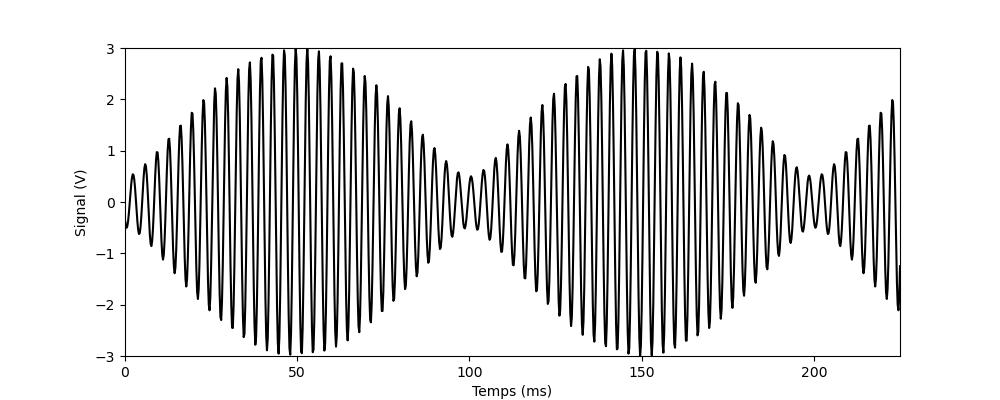
\includegraphics[width=0.95\textwidth]{propagation/battements.jpg}
\end{exercise}

\begin{solution}
Pour les fréquences, la porteuse a une demi-période de 100 ms et l'oscillation rapide fait 15 oscillations en 50 ms soit d'où $f_1 + f_2 = 600$~Hz et $f_1-f_2 = 10$~Hz et donc $f_1 = 295$~Hz et $f_2 = 305$~Hz.

Pour les amplitudes, $A_1 + A_2 = 3$ et $A_1- A_2 = 0.5$ d'où $A_1 = 1.25$ V et $A_2 = 1.75$ V
\end{solution}
% Niveau :      PC
% Discipline :  Méca
% Mots clés :   Pont suspendu

\begin{exercise}{Pont suspendu}{2}{Sup, Spé}
{Mécanique, Ondes mécaniques, Corde}{bermu}

Soit un pont suspendu enjambant un bras de mer, maintenu par un câble de poids négligeable attaché à deux poteaux de hauteur $H$ plantés de part et d'autre du pont et séparés d'une longeur $L$.

\begin{figure}[H]
    \centering
    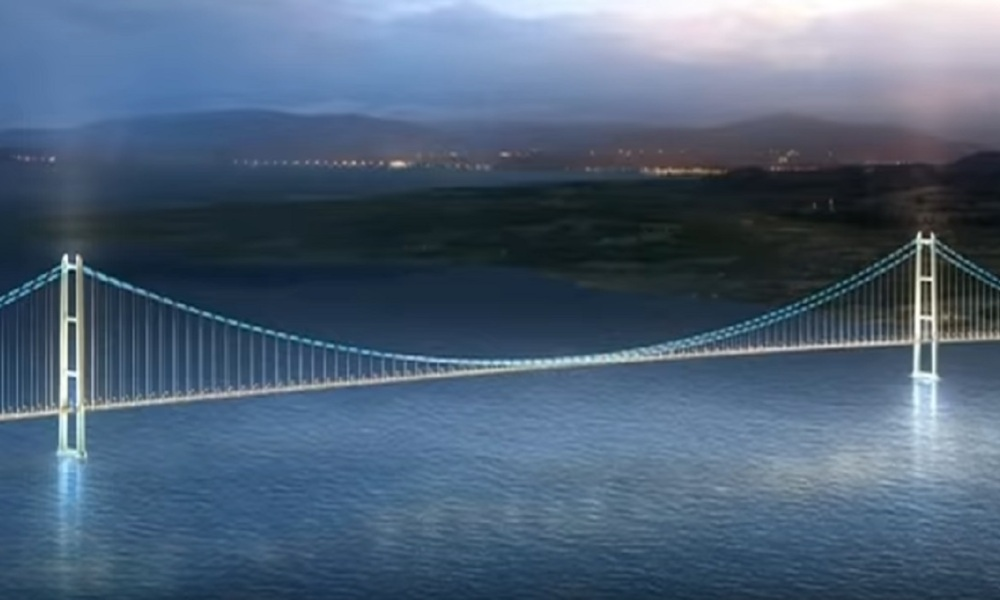
\includegraphics[height=15em]{meca/ondes_meca/pont-suspendu.jpeg}
    \caption{Vision d'artiste du projet du plus grand pont suspendu du monde, en Turquie.}
\end{figure}

\begin{questions}
\question Donner l'équation décrivant la forme du câble.
\uplevel{On s'intéresse maintenant au tablier du pont (la partie où se trouve la route) qui, lorsque le pont est au repos, est horizontal.}
\question Montrez que la hauteur du tablier vérifie une équation d'onde. On précisera la célérité associée.
\question Dans quel cas le tablier peut-il entrer en résonance ? Citer un cas célèbre où un tel phénomène s'est produit.
\end{questions}

\paragraph{Données :}  L’abscisse curviligne $s$ est telle qu’un élément de longueur de la corde $\dd{s}$ de la courbe vérifie
\begin{align*}
    \dd{s}^2 = \dd{x}^2 + \dd{z}^2 &= \qty(1+ z'(x)^2)\dd{x}^2.
\end{align*}
\end{exercise}
% Niveau :      PC
% Discipline :  Méca
% Mots clés :   Chaînette

\begin{exercise}{Chaînette}{3}{Spé}
{Mécanique,Ondes mécaniques,Corde}{bermu}

Soit une chaînette homogène de masse linéique $\mu_\ell$, fixée en $\pm L/2$ à une altitude $H$.

À quelle condition la chaînette touche le sol à $z = 0$ ? Donner des systèmes physiques réels ayant un tel comportement et estimer les paramètres intervenants.

\paragraph{Données :} L’abscisse curviligne $s$ est telle qu’un élément de longueur de la corde $\dd{s}$ de la courbe vérifie
\begin{align*}
    \dd{s}^2 = \dd{x}^2 + \dd{z}^2 &= \qty(1+ z'(x)^2)\dd{x}^2. \\
    \mathrm{argsinh}'(x) &= \dfrac1{\sqrt{1+x^2}}.
\end{align*}
\end{exercise}
% Niveau :      PC
% Discipline :  Méca
% Mots clés :   Chaine, caténaire

\begin{exercise}{Les caténaires du TGV}{3}{Spé}
{Mécanique, Ondes mécaniques, Corde}{potier}

Le TGV (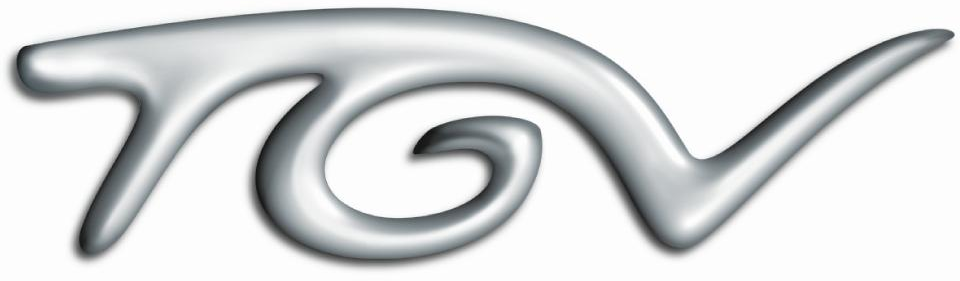
\includegraphics[height=1em]{meca/ondes_meca/TGV.png}) est alimenté en électricité par un pantographe (bras articulé) qui doit rester en contact avec la caténaire (le câble électrique d’alimentation) au cours du déplacement du train. Sur un ligne classique, ce câble est un câble de cuivre pur, tendu, dont la section vaut $150$  mm$^2$.

Montrer que quelles que soient les performances des moteurs électriques, la vitesse
du TGV est limitée par une limite physique qu’on évaluera.

On rappelle que le record actuel de vitesse du TGV est de $574,8$ km$\cdot$h$^{-1}$ en 2007.

Quelles solutions techniques à apporter pour augmenter cette vitesse limite sans que le 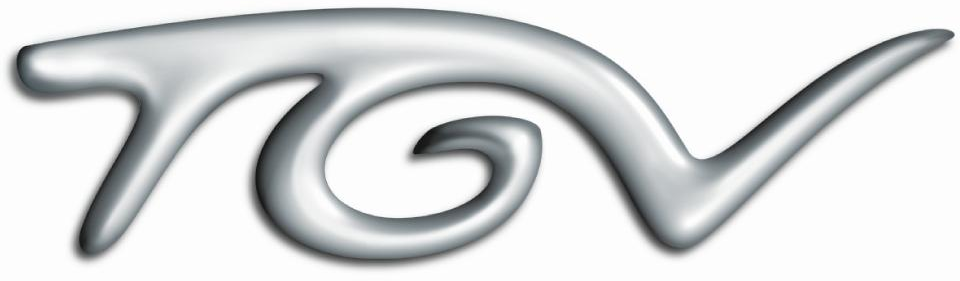
\includegraphics[height=1em]{meca/ondes_meca/TGV.png} ne se transforme en 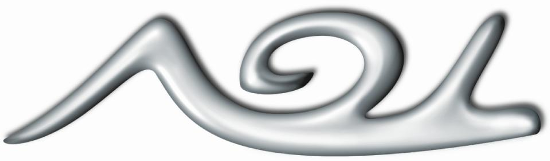
\includegraphics[height=1em]{meca/ondes_meca/GTV.png}...
\end{exercise}
% Niveau :      PCSI
% Discipline :  Méca

\begin{exercise}{Corde verticale}{3}{Spé}
{Mécanique,Ondes mécaniques,Corde}{lelay}

Le but de cet exercice est de modéliser les mouvements d'une corde soumise à une excitation sinusoïdale. On commence par étudier les mouvements selon l'axe $y$ d'une corde de longueur $L$, tendue entre deux points placés sur l'axe $x$ avec une tension $T_0$. 
\begin{questions}
    \questioncours Équation de D'Alembert et notion d'impédance.
    \question Montrez que l'on peut au premier ordre modéliser les petits mouvements de la corde par une équation de D'Alembert. Quelle est la célérité associée ?
    \question Faire apparaître une "impédance mécanique", en considérant les variables $v_y$ et $T_y$.
    \uplevel{On étudie maintenant les mouvements transversaux d'une corde verticale accrochée un plafond ($z=0$), de masse $m$ et de longueur $L$.}
    \question Déterminer $T_0(z)$ la tension de la corde au repos.
    \question Déterminer l'équation de propagation dans la corde.
    \question L'extrémité de la corde en $z=L$ est libre de se mouvoir. On suppose que l'on impose un petit mouvement transversal à la corde $y(0,t) = y_0\cos(\omega t)$.
    \begin{parts}
        \part Justifier que l'on cherche les solutions sous la forme $y(z,t) = f(z)\cos(\omega t)$
        \part Établir l'équation différentielle vérifiée par $f$. L'adimensionner en utilisant comme longueur caractéristique $g/\omega^2$.
        \part La suite de cet exercice n'a pas encore été écrite, mais bravo si vous êtes arrivé jusque là !
    \end{parts}
\end{questions}
\end{exercise}
% Niveau :      PC
% Discipline :  Méca
% Mots clés :   Ressort, Impureté, Chaines

\begin{exercise}{Impureté dans un cristal}{2}{Spé}
{Mécanique, Ondes mécaniques, Ressort}{potier,bermu}

On considère une chaîne infinie linéaire d’atomes ponctuels de masse $m$ liés par des ressorts de raideur $K$. La chaîne est portée par l’axe $OX$ ; à l’équilibre, les atomes occupent les positions $x_n = n a$ avec $n\in\mbb{Z}$, où $a$ est la longueur à vide des ressorts. En $X=0$ se trouve une impureté (atome de masse $M$).
\begin{figure}[H]
    \centering
    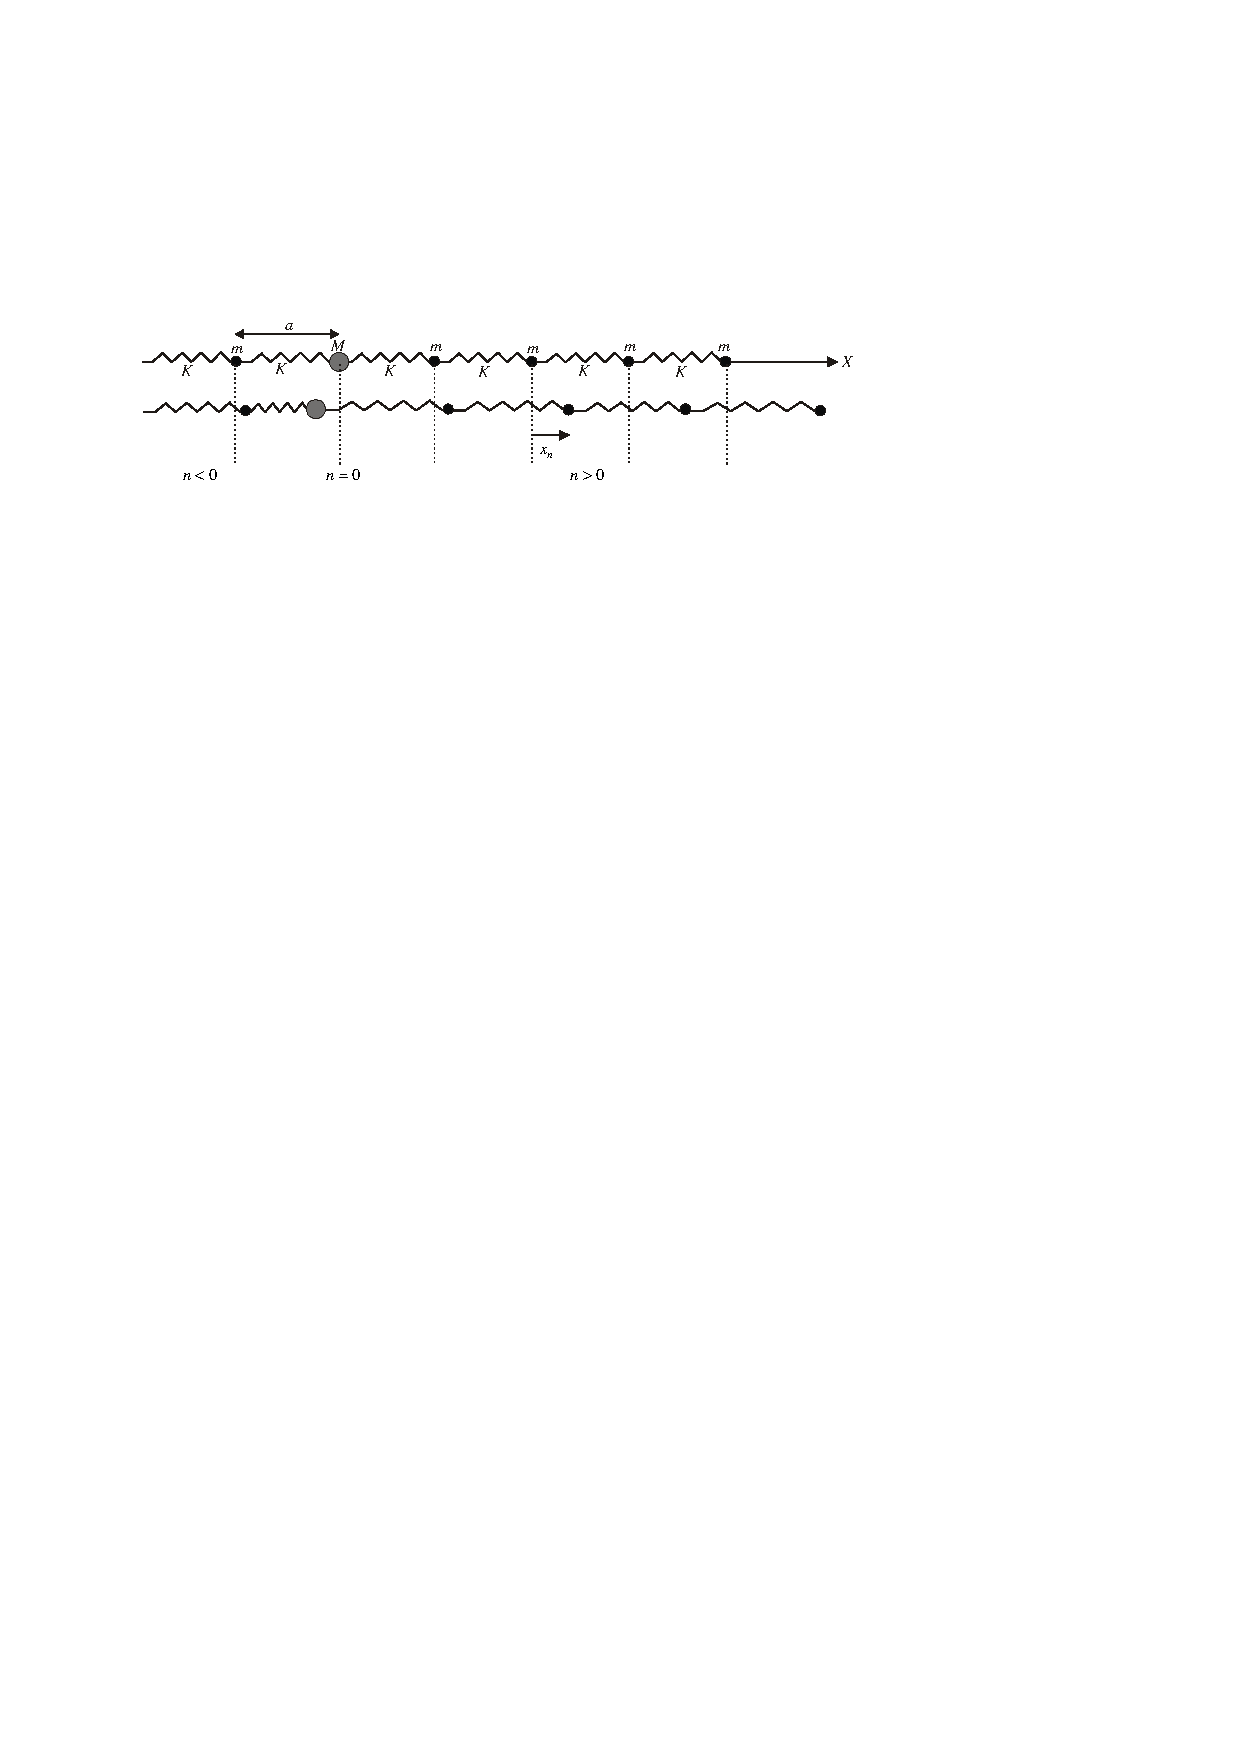
\includegraphics[width=\linewidth]{meca/ondes_meca/impurete.pdf}
    \vspace{-1.5em}
    \caption{Modèle de l'impureté dans un cristal par une chaine de ressorts.}
\end{figure}

\begin{questions}
\question (\emph{Préliminaire}) Quel sens physique peut-on donner à $m$, $K$ et $a$ ? Dans quelle limite le modèle de la chaîne de ressorts est valable ? Estimer en ordre de grandeur ces quantités.
\question Établir le système d'équations différentielles régissant l'écart à l'équilibre $x_n$ de l’atome $n$ par rapport à sa position d’équilibre.

\uplevel{On cherche des solutions sous la forme $\underline{x_n}(t) = A e^{i(\omega t -  k X_n)}$ dans la partie $X_n<0$, avec $A\in\mbb{R}$.}
\question Montrer que $k$ et $\omega$ sont liés par une relation de dispersion.
\question Montrer que si l’on considère une onde progressive incidente $\underline{x_n}(t) = A e^{i(\omega t -  k X_n)}$ dans la partie $X_n<0$, il y a nécessairement en $X=0$ une onde réfléchie d’amplitude $B$ et une onde transmise d’amplitude $C$.\\
Déterminer ces amplitudes complexes en fonction de A.
\question Étudier les cas
\begin{parts}
\part $M \gg m$,
\part $M \ll m$,
\part $\abs{M - m} \ll m, M$.
\end{parts}
Interpréter ces résultats.
\question On se place dans le cas où $M = m$ : il n’y a pas de défaut. \\
Montrer que la chaîne se comporte comme un filtre passe-bas dont on calculera la pulsation de coupure $\omega_c$ . Tracer le graphe $\omega(k)$. \\
On interprétera en particulier $x_n$ dans les cas limites
\begin{parts}
\part $\omega \ll \omega_c$,
\part $\abs{\omega - \omega_c} \ll \omega, \omega_c$.
\end{parts}
\question Déterminer alors la vitesse de phase et la vitesse de groupe
de l’onde. Montrer que l’on peut déterminer dans ce cas une équation d’onde et retrouver les résultats précédents.
\end{questions}
\end{exercise}
% Niveau :      PC
% Discipline :  Méca
% Mots clés :   Ondes

\begin{exercise}{Ondes sismiques}{3}{Spé}
{Mécanique, Ondes mécaniques, Ondes sismiques}{bermu}

\begin{questions}
    \questioncours Par analogie avec un système de ressorts en série, quelle est le comportement d'un solide élastique. \\
    On pourra utiliser le module d'Young $E$.
\end{questions}

Idée : faire redémontrer la propagation d'ondes anisotrope ondes S et P et faire un peu de géométrie en mode hodochrones.

\end{exercise}
% Niveau :      PCSI
% Discipline :  Ondes
%Mots clés :    

\begin{exercise}{Modélisation du traffic}{2}{Sup, Spé}
{Ondes}{lelay}

\begin{questions}
    \questioncours Soit une grandeur extensive de densité $\rho(\vx,t)$. Cette grandeur est mue par une densité de flux $\boldsymbol{\varphi}$. Donnez l'équation de conservation de cette grandeur puis comparez plusieurs exemples usuels en explicitant la forme de $\boldsymbol{\varphi}$.
\begin{EnvUplevel}
Nous allons par la suite modéliser le trafic routier 1D à l'aide d'une équation de conservation.
\end{EnvUplevel}
    \question Proposez une grandeur physique à laquelle on applique l'équation de conservation.
    \question On suppose que le flux de voitures obéit se déplace localement à la vitesse suivante
    $$u(\rho) = u_\text{max}\qty(1 - \dfrac{\rho}{\rho_\text{c}}).$$
    Identifiez le sens physique de cette expression en considérant les cas limites. \question Quel est le flux $\varphi$ associé ? En déduire l'équation de la dynamique du système.
    \question Adimensionnez ce modèle.
\uplevel{Par la suite, les variables désignent les quantités adimensionnées.}
    
    \question On considère tout d'abord que le traffic est très fluide $\rho \ll 1$.
    \begin{parts}
        \part Donnez à l'ordre principal en $\rho$ l'équation de la dynamique du système et résolvez-là avec la situation générale
        $$\rho(x, t=0) = \rho_0(x).$$
        On pourra considérer le changement de variable $z = x - t$.
        \part Faire un schéma pour une distribution gaussienne de voitures.
        \part Représenter la relation de dispersion du milieu et considérez les cas limites que ne prennent pas en compte l'appoximation $\rho\ll 1$.
    \end{parts}
    
    A finir !
    
\end{questions}

\paragraph{Données :}
\begin{itemize}
    \item accélération de la pesanteur terrestre $g = 10$ m$^2\cdot$s$^{-1}$,
    \item masse volumique de l'acier $\rho = 8\cdot 10^3$ $\mathrm{kg\cdot m^{-3}}$,
    \item hauteur de la tour Eiffel $H = 300$ m,
    \item largeur de la base de la tour Eiffel $L = 125$ m.
\end{itemize}
\end{exercise}

\section{Mécanique en référentiel non galiléen}
% Niveau :      Spé
% Discipline :  Méca
% Mots clés :   Chaine, caténaire

\begin{exercise}{Analogie RMN et pendule en rotation}{2}{Spé}
{Mécanique,Mécanique en référentiel non galiléen,Pendule}{bermu}

\begin{questions}
    \questioncours Forces d'inertie d'entraînement et de Coriolis.
\begin{EnvUplevel}
Considérons un pendule rigide de longueur $\ell$ et de masse $m$ fixé en $O$ dans un champ de pesanteur $\vg = -g\ve_z$. Le pendule se trouve dans un référentiel $\cal{R}'$ en rotation uniforme à la vitesse $\Omega$ autour de l'axe $\ve_z$. \\
On se placera dans un système de coordonnées sphériques $(r,\theta,\varphi)$ où $\theta\in\qty[0,\pi]$ est l'angle entre $Oz$ et l'axe du pendule.
\end{EnvUplevel}
    \question Chercher les positions d'équilibre du pendule $\theta_\text{eq}$, ainsi que leur stabilité. \\
    On ne fera intervenir que la fréquence propre du pendule $\omega_0$ et la fréquence de rotation $\Omega$.
    \question Tracer pour plusieurs valeurs pertinentes de $\Omega$ le profil d'énergie potentielle ainsi que les positions d'équilibre stables et instables. Interpréter les différentes zones de ce graphe.
    \uplevel{Nous allons maintenant étudier la dynamique locale du pendule proche des positions d'équilibre.}
    \question Pour chaque position d'équilibre $\theta_{\text{eq}, i}$, en substituant $\theta$ dans l'équation de la dynamique du pendule par
    $$\theta = \theta_{\text{eq}, i} + \varepsilon_i,$$
    montrer que pour de faibles variations $\varepsilon_i$ autour de la position d'équilibre, l'équation de la dynamique devient à l'ordre 1 en $\varepsilon_i$
    \begin{itemize}
        \item celle d'un oscillateur harmonique classique de pulsation $\omega_i$, si elle est stable,
        \item celle d'un système exponentiellement divergent avec taux de croissance $\sigma_i$, si elle est instable.
    \end{itemize}
    Interpréter physiquement ces deux résultats en discutant notamment des limites du modèle.
    Tracer $\theta_{\text{eq}, i}$, $\omega_i$ et $\sigma_i$ en fonction de $\Omega$ et interpréter.
\end{questions}
\paragraph{Questions facultatives (niveau PC) :}
\begin{questions}
    \question Rappeler ce qu'est la précession de Larmor et dresser une analogie avec le système précédent.
    \question Rappeler ce qu'est une transition de phase, ou changement d'état. \\
    En quoi peut-on dire que ce système effectue une transition de phase à la pulsation $\omega_c$ ?
\end{questions}

\end{exercise}
% Niveau :      Spé
% Discipline :  Méca
% Mots clés :   Chaine, caténaire

\begin{exercise}{Pendule de Foucault}{3}{Spé}
{Mécanique,Mécanique en référentiel non galiléen,Pendule,Coriolis}{bermu}

\begin{questions}
    %\questioncours Caractère galiléen approché des référentiels héliocentrique, de Copernic, géocentrique et terrestre. \\
    %On appuiera la démonstration d'ordres de grandeur et on estimera la contribution des forces d'inertie dans un problème de dynamique terrestre.
    \questioncours Forces d'inertie d'entraînement et de Coriolis.
    %\question Montrer que sur Terre, à une lattitude $\lambda$ donnée, l'accélération d'inertie d'entraînement agit comme une correction sur $\vec{g}_0\mapsto\vec{g}$, dont on donnera l'ordre de grandeur. Quel est l'angle entre $\vec{g}_0$ et $\vec{g}$ ?

\begin{EnvUplevel}
On se propose d'étudier l'expérience effecutée par Léon Foucault en 1851 à Paris sur les effets du caractère non galiléen du référentiel terrestre sur la dynamique d'un pendule.

Soit un pendule simple, constitué d’une corde de très grande longueur $L$ de masse négligeable, suspendue en un point fixe $B$ du repère terrestre, et au bout de laquelle oscille un point matériel $M$ de masse~$m$. Soit $\lambda$ la latitude du lieu.

On étudie le mouvement du point $M$ dans le référentiel terrestre $\scr{R}$ lié au repère $(A ; x, y,z)$ centré sur la position d’équilibre $A$ du point $M$, $Az$ étant la verticale ascendante du lieu, $Ax$ dirigé vers le nord et $Ay$ vers l'est. On néglige tout frottement.
\end{EnvUplevel}
    \questionbonus Culture scientifique : contributions scientifiques de Léon Foucault.
    \question En précisant bien quels référentiels vous utilisez, effectuer un bilan des forces détaillé sur $M$.
\uplevel{Dans l’hypothèse de petites oscillations autour de la verticale locale $(Az)$, on a en première approximation que le mouvement s’effectue dans le plan $(A ; x, y)$ et que la composante suivant $Oz$ de la résultante des forces est nulle. On introduit donc $\Big.\vec{\xi} \deq x\ve_x + y\ve_y$, la projection de $M$ dans le plan $(A ; x, y)$.}
    \question Justifiez cette hypothèse et montrez qu'on a par conséquent que dans le plan $(A ; x, y)$
    \begin{align*}
        &\textsf{(a)}& \vec{T} & \propto \vec{AM} \simeq - m\omega_0^2 \vec{\xi}, &&\\
        &\textsf{(b)}& \vec{F}_\textsc{c} &\simeq -m f \ve_z \cross\dv{\vec{\xi}}{t},&&
    \end{align*}
    où $\vT$ est la tension de la corde, $\vec{F}_\textsc{c}$ la force de Coriolis, et $\omega_0$ et $f$ des quantités constantes (le justifier) dont on donnera les expressions, le sens physique et les ordres de grandeur.
    
    \question En déduire que l’équation vectorielle du mouvement projeté dans le plan horizontal $(A ; x, y)$ est
    $$\dv[2]{\vec{\xi}}{t} = -{\omega_0}^2\vec{\xi} - f \ve_z\cross\dv{\vec{\xi}}{t}$$
    et interpréter chaque terme.
    \question Montrez que si l'on se place dans un référentiel $\scr{R}'$ en rotation autour de l'axe $Oz$ par rapport à $\scr{R}$ à une pulsation $\omega_\textsc{c}$ bien choisie, on obtient l'équation d'un oscillateur harmonique.
    %$$\dv[2]{\vec{\xi}'}{t} = -{\omega_0}^2\vec{\xi}'.$$
    En déduire que le pendule oscille dans un plan tournant à une vitesse angulaire qu'on donnera.
\end{questions}
\paragraph{Données historiques :} pendule du Panthéon, $L = 67$ m et $\lambda = 49^\circ$.
On note $\omega_\textsc{t}$ la pulsation associée à la rotation de la Terre.

\noindent\textsf{Nota :} la latitude $\lambda$ est l'angle depuis l'équateur jusqu'au point étudié.
\end{exercise}


\begin{solution}

\begin{questions}
    \setcounter{question}{2}
    \question On se place dans $\scr{R}$, en translation circulaire autour
\end{questions}

\end{solution}
% Niveau :      Spé
% Discipline :  Méca
% Mots clés :   Chaine, caténaire

\begin{exercise}{Gravimétrie terrestre}{3}{Spé}
{Mécanique,Mécanique en référentiel non galiléen,Pesanteur,Gravité,Forces d'inertie}{bermu}

\begin{questions}
    \questioncours Caractère conservatif de la force d'inertie d’entraînement et champ de pesanteur dans un référentiel non galiléen. 
    
\begin{EnvUplevel}
On considère le référentiel terrestre qui se situe en surface de la Terre à la latitude $\lambda$.

\end{EnvUplevel}
    \question \textsf{Question ouverte :} le champ de pesanteur $g$ varie plus significativement si on se déplace de $h = \SI{1}{m}$ vers le nord, vers l'est, ou en altitude ? \`A quelle conditions peut-on estimer que $g$ est constant ?
\end{questions}
\paragraph{Notations :} 
On note $\Omega_\textsc{t}$ la pulsation associée à la rotation de la Terre, et $R_\textsc{t}$ son rayon.

\hspace{4.3em}
On note $\lambda$ la latitude qui est l'angle entre l'équateur et point le étudié ($\lambda = 49^\circ$ à Paris).
\end{exercise}

\begin{solution}
\begin{questions}
    \questioncours $$\vec{g} = \vec{g}_0 + \vec{a}_\text{ie} = -\dfrac{GM}{(R_\textsc{t}+z)^2}\vec{e}_z + \Omega^2_\textsc{t} R_\textsc{t} \cos\lambda \vec{e}_h = -\grad\qty(\dfrac{GM}{R_\textsc{t}+h} + \dfrac{1}{2}\Omega^2_\textsc{t} R_\textsc{t}^2 \cos\lambda^2),$$
$\vec{e}_z$ étant la verticale locale (depuis le centre de la Terre) et $\vec{e}_h$ le projeté orthogonal depuis l'axe de rotation de la Terre.
    \question
    \begin{itemize}
        \item \textsf{Variation selon $y$ :} nulle
        \item \textsf{Variation selon $z$ :}
        $$\delta g \simeq \delta\qty(-\dfrac{GM}{(R_\textsc{t}+h)^2}) = g_0 \dfrac{2 \delta z}{R_\textsc{t}} \qquad \dfrac{\delta  g}{g_0} \simeq \SI{3e-7}{}$$
        Raisonnable donc pour $\delta z \ll R_\textsc{t}$.
        \item \textsf{Variation selon $x$ :}
        $$\delta g \simeq \delta\qty(\Omega^2_\textsc{t} R_\textsc{t} \cos\lambda) = \Omega^2_\textsc{t} R_\textsc{t} \sin\lambda \delta\lambda = \Omega^2_\textsc{t} \sin\lambda \delta x \qquad \dfrac{\delta  g}{g_0} \simeq \SI{4e-10}{}$$
        Toujours raisonnable car $a_\text{ie}/g_0 \simeq \SI{5e-3}{}$ au max.
    \end{itemize}
\end{questions}
\end{solution}

% Niveau :      Spé
% Discipline :  Méca
% Mots clés :   Chaine, caténaire

\begin{exercise}{Expérience de Cassini}{3}{Spé}
{Mécanique,Mécanique en référentiel non galiléen,Chute libre,Déviation vers l'est}{bermu}

\begin{questions}
    \questioncours Caractère galiléen approché du référentiel terrestre. \\
    On appuiera la démonstration d'ordres de grandeur et on estimera la contribution des forces d'inertie dans un problème de dynamique terrestre.
    

\begin{EnvUplevel}
On se propose d'étudier l'expérience effectuée par Cassini en 1679 à l'observatoire de Paris sur les effets du caractère non galiléen du référentiel terrestre sur la chute libre d'un corps de masse $m$, supposé ponctuel, lâché sans vitesse dans un puits de profondeur $h$, et situé à la latitude $\lambda$.

On se placera dans le repère $(O,x,y,z)$ placé à la surface de la Terre, $Ox$ pointant vers le nord et $Oy$ vers l'ouest.

\end{EnvUplevel}
    \question Donner les équations de la dynamique de la particule, projetées sur chaque axe.
    \question Considérant que les effets non-galiléens son faibles, simplifier l'équation de sorte à ce qu'il n'y ait qu'un terme de force suivant chaque composante et résoudre l'équation.
    \question \`A l'observatoire de Paris (lattitude $\lambda = 49^\circ$), dans un puits de $h = \SI{158}{m}$ de profondeur,\linebreak Cassini a mesuré une déviation vers l'est de $y = 28$ mm vers l'est. Interpréter.
    \questionbonus Montrer également qu'on devrait observer une faible déviation vers le sud.
\end{questions}
\paragraph{Notations :} 
On note $\Omega_\textsc{t}$ la pulsation associée à la rotation de la Terre, et $R_\textsc{t}$ son rayon.

\hspace{4.3em}
On note $\lambda$ la latitude qui est l'angle entre l'équateur et point le étudié ($\lambda = 49^\circ$ à Paris).\end{exercise}

\begin{solution}
\begin{questions}
    \questioncours Dynamique inférieure à 24 heures.
    \question 
    $$\dv{\vv}{t} = -g\vec{e}_z - 2\vec{\Omega}_\textsc{t}\cross\vv = -g\mqty(0,0,1) - 2\Omega_\textsc{t} \mqty(\cos\lambda\\0\\-\sin\lambda)\cross\mqty(\dot{x}\\\dot{y}\\\dot{z}).$$

    $$\left\lbrace\begin{array}{l}
        \ddot{x} = 2\Omega_\textsc{t} \sin\lambda \dot{y}  \\
        \ddot{y} = 2\Omega_\textsc{t} (\sin\lambda \dot{x} + \cos\lambda \dot{z})  \\
        \ddot{z} = -g - 2\Omega_\textsc{t} \cos\lambda \dot{y}
    \end{array}\right.$$
    \question Or on a $\dot{x}$ et $\dot{y}$ négligeables, donc :
    $$\left\lbrace\begin{array}{l}
        \ddot{x} = 2\Omega_\textsc{t} \sin\lambda \dot{y}  \\
        \ddot{y} = 2\Omega_\textsc{t} \cos\lambda \dot{z}  \\
        \ddot{z} = -g
    \end{array}\right.$$
    d'où
    \begin{align*}
        \ddot{z} &= -g &
        \dot{z} &= -gt &
        z &= -\dfrac{1}{2}gt^2 \\
        \ddot{y} &= -2\Omega_\textsc{t} \cos\lambda g t &
        \dot{y} &= -\Omega_\textsc{t} \cos\lambda g t^2 &
        y &= - \dfrac{1}{3}\Omega_\textsc{t} \cos\lambda g t^3 \\
        \ddot{x} &= -2\Omega_\textsc{t}^2 \cos\lambda \sin\lambda g t^2 &
        \dot{x} &= -\dfrac{2}{3}\Omega_\textsc{t}^2 \cos\lambda \sin\lambda g t^3 &
        x &= -\dfrac{1}{6}\Omega_\textsc{t}^2 \cos\lambda \sin\lambda g t^4
    \end{align*}
    or $t = \sqrt{\dfrac{2h}{g}}$ d'où
    $$\left\lbrace\begin{array}{l}
        x =  -\dfrac{2}{3}\Omega_\textsc{t}^2 \cos\lambda \sin\lambda \dfrac{h^2}{g} \\
        y = - \dfrac{1}{3}\Omega_\textsc{t} \cos\lambda g \qty(\dfrac{2h}{g})^{3/2} \\
        z = - h
    \end{array}\right.$$
    \question On introduit une longueur typique :
    $$\ell = \dfrac{g}{\Omega_\textsc{t}^2} \simeq \SI{1,8e9}{m}$$
    $$\left\lbrace\begin{array}{l}
        x =  -\dfrac{2}{3} \cos\lambda \sin\lambda \dfrac{h^2}{\ell} \\
        y = - \dfrac{2\sqrt{2}}{3} \cos\lambda h \sqrt{\dfrac{h}{\ell}} \\
        z = - h
    \end{array}\right.$$
    On retrouve bien l'ODG.
    \question Pour $x$ on trouve une déviation vers le sud de $x = \SI{0,13}{um}$
\end{questions}
\end{solution}
% Niveau :      Spé
% Discipline :  Méca
% Mots clés :   Chaine, caténaire

\begin{exercise}{Attention fragile ! (dans le camion)}{2}{Spé}
{Mécanique,Mécanique en référentiel non galiléen,Frottements}{bermu}


\textsf{Question de cours :} Lois du frottement solide de Coulomb.

Lors d'un déménagement, vous transportez vos cartons avec un camion.
Vous craignez qu'une conduite brusque entraîne les cartons à se cogner contre les parois du camion.

\textsf{Question ouverte :} Estimez l'accélération maximale du camion permettant de ne pas casser la vaisselle contenue dans un carton. (\textsl{On pourra s'aider des indications ci-après})

\paragraph{Indications}

\begin{enumerate}
    \item Modéliser la situation de manière simple : un carton de masse $m$, dans un camion de longueur $L$ allant à une accélération constante $\gamma$ et estimer à quelle condition se produit le glissement du carton.
    \item Estimer l'énergie nécessaire à briser la vaisselle dans le carton à partir de considérations simples.
    \item Estimer l'énergie acquise par le carton avant le choc contre la paroi du camion.
    \item Comparer à l'accélération typique d'un véhicule.
\end{enumerate}

On estimera par des ordres de grandeur pertinents les quantités physiques du problème.

\end{exercise}

\begin{solution}
Dans le référentiel en accélération :
    $$m\dv{\vec{v}}{t} = -mg\vec{e}_z + N\vec{e}_z + T\vec{e}_x - m\gamma\vec{e}_x$$
Avec $N = mg$.

Les lois de Coulomb donnent :
\begin{itemize}
    \item en statique : $v = 0$, $T = m\gamma < f_s N = f_s m g$ soit $\gamma < f_s g$ \\
    \noindent il y a donc une première accélération critique qui est $\gamma_\text{c1} = f_s g$.
    \item en dynamique : $T = f_d N$ donc $\ddot{x} = -\gamma + f_d g$
\end{itemize}

Donc on accumule une énergie $E = m L (\gamma - f_d g)$.

On estime que l'énergie nécessaire à fracasser la vaisselle est celle donnée par une chute de $H = 1$~m.

Donc $\gamma_\text{c2} = g\qty(f_sd + \dfrac{H}{L})$.

ODG :


L'angle de glissement limite pour un carton est de l'ordre de 10$^\circ$ donc $f \sim 0.2$ et $\gamma_\text{c1} \sim 0.2g$.

$L = 5$ m. Donc $\gamma_\text{c2} = 0.4$.

$\gamma = 0.3$ g pour un véhicule.

Il faudra donc être prudent.


\end{solution}

% Niveau :      Spé
% Discipline :  Méca
% Mots clés :   Chaine, caténaire

\begin{exercise}{Attention fragile ! (avec la brouette)}{2}{Spé}
{Mécanique,Moment cinétique,Frottements}{bermu}


\textsf{Question de cours :} Lois du frottement solide de Coulomb.

Lors d'un déménagement, vous transportez vos cartons avec une brouette.
Vous craignez que pencher trop la brouette fasse glisser ou se renverser le carton.

\textsf{Question ouverte :} Estimez les angles à partir desquels le carton se renverse ou glisse.

\paragraph{Indications}~\\

On modélisere la situation de manière simple : un carton de masse $m$, de hauteur $H$ et de longueur de largeur identiques $L$, posé sur un plan incliné d'un angle $\theta$ en étudiant :
\begin{enumerate}
    \item Etudier la situation du glissement.
    \item Etudier la situation du versage.
\end{enumerate}

On estimera par des ordres de grandeur pertinents les quantités physiques du problème.

\end{exercise}

\begin{solution}
On a dans le référentiel penché :
    $$m\dv{\vec{v}}{t} = m\vec{g} + N\vec{e}_y + T\vec{e}_x$$
Avec $\vec{g} = -g(\cos\theta\vec{e}_y + \sin\theta\vec{e}_x)$

Les lois de Coulomb donnent :
\begin{itemize}
    \item en statique : $v = 0$, $T = m g \sin\theta < f_s N = f_s m g \cos\theta$ soit $\tan\theta < f_s$ \\
    \noindent il y a donc l'angle de glisement qui est $\theta_\text{g} = \tan^{-1}f_s$.
\end{itemize}

Pour le glissement, on applique le TMC au point inférieur du carton $A$.

$$J = \dfrac{m}{HL^2} \iiint \dd{x}\dd{y}\dd{z} (x^2+y^2) = \dfrac{1}{3}m(L^2+H^2)$$

$$\scr{M}^{Oz}_{T} = \scr{M}^{Oz}_{R} = \vec{0}$$

$$\scr{M}^{Oz}_{m\vec{g}} = \dfrac{m}{HL^2z} \iiint \dd{x}\dd{y}\dd{z} \vec{r}\cross\vg = m\vec{\text{AG}}\cross\vec{g} = \dfrac{mg}{2}(L \cos\theta - H\sin\theta) =  -\dfrac{mg}{2}\sqrt{L^2+H^2}\sin(\theta-\theta_\text{b}),$$
avec G le barycentre du système et $\theta_\text{b} = \tan^{-1}\dfrac{L}{H}$.

Le système basculera donc si on passe l'angle de basculement $\theta_\text{b}$
\end{solution}
% Niveau :      Spé
% Discipline :  Méca RNG

\begin{exercise}{Bague sur un cerceau centré}{2}{Spé}
{Mécanique,Mécanique en référentiel non galiléen}{lelay, classique}

\begin{questions}
    \questioncours Forces de frottement solides et fluides.
\begin{EnvUplevel}
On considère une bague de masse $m$ enfilée sur un cerceau rigide, qui tourne à vitesse angulaire $\Omega$ autour de son axe de symétrie vertical.
\end{EnvUplevel}
    \question Quel type de frottement intervient entre la bague et le cerceau ? On les négligera par la suite.
    \question Donner l'équation du mouvement de la bague et interpréter qualitativement l'influence de chaque terme sur sa dynamique. On fera intervenir une pulsation caractéristique $\omega_0$ convenablement choisie.
    \question Combien de positions d'équilibre de la bague y a-t-il ? De quoi dépend ce nombre ?
    \question Indiquer la (les) positions d'équilibre(s) de la bague en fonction du paramètre $\mu = \frac{\Omega^2}{\omega_0^2}$. Pour chaque position d'équilibre, donner la condition de stabilité.
    \question Montrer que toutes les forces considérées ici dérivent d'un potentiel et donner la forme de l'énergie potentielle totale $E_p$ de la bague.
    \question Tracer pour plusieurs valeurs pertinentes de $\mu$ le profil d'énergie potentielle et indiquer les positions d'équilibre stables et instables. Identifier les "bassins d'attraction" des points fixes stables.
    \question Pourquoi parle-t-on d'une "bifurcation" ou "transition de phase" du système en $\mu = 1$ ? 
\end{questions}
\end{exercise}
% Niveau :      Spé
% Discipline :  Méca RNG

\begin{exercise}{Bille dans un récipient conique}{2}{Spé}
{Mécanique,Mécanique en référentiel non galiléen}{lelay}

\begin{questions}
    \questioncours Forces conservatives et conservation de l'énergie.
\begin{EnvUplevel}
On considère une bille de masse $m$ libre de rouler sans frottements sur la surface d'un cône d'angle au sommet $\alpha$ renversée dans lequel elle est posée. Ce cône tourne à une fréquence $\Omega$ autour de son axe de révolution, et la bille tourne avec lui de manière synchronisée.
\end{EnvUplevel}
    \question On suppose qu'au départ la bille se trouve à une distance $\ell_0$ de la pointe du cône. Indiquer la condition sur $g$, $\Omega$, $\alpha$ que doit vérifier $\ell_0$ pour que la bille soit à l'équilibre. 
    \question Dire qualitativement si l'équilibre considéré est stable ou instable.
    \question On suppose maintenant que la bille posée sans vitesse initiale à une distance $\ell = \ell_0 - \epsilon$ du sommet. Comment va varier $\ell$ en fonction du signe de $\epsilon$ ?
    \question En considérant $\epsilon \ll 1$, donner le temps que va mettre la bille à retomber au sommet du cône.
    % \question On se place maintenant exactement en $\ell = \ell_0$ et on donne une petite pichenette à la bille afin de lui donner une petite vitesse $\nu$. Comment va varier $\ell$ en fonction du signe de $\nu$ ?
    % \question En considérant $\\nu \ll 1$, donner le temps que va mettre la bille à sortir du cône (on considère que le cône est de taille $L$^). Quelle sera sa vitesse $v_s$ au moment de sortir ?
    % \question Calculer la trajectoire de la bille après sa sortie dans le référentiel tournant puis dans le référentiel du laboratoire
\end{questions}
\end{exercise}
% Niveau :      Spé
% Discipline :  Méca RNG

\begin{exercise}{Bague sur un cerceau non centré}{2}{Spé}
{Mécanique,Mécanique en référentiel non galiléen}{lelay}

\begin{questions}
    \questioncours Forces d'inertie d'entraînement et de Coriolis.
\begin{EnvUplevel}
On considère une bague de masse $m$ enfilée sur un cerceau rigide, qui tourne à vitesse angulaire $\Omega$ autour d'un axe vertical lui étant tangent. Tous les frottements sont ici négligés.
\end{EnvUplevel}
    \question Donner l'équation du mouvement de la bague et interpréter qualitativement l'influence de chaque terme sur sa dynamique. On fera intervenir une pulsation caractéristique $\omega_0$ convenablement choisie.
    \question Combien de positions d'équilibre de la bague y a-t-il ?
    \question Donner la position d'équilibre de la bague en fonction du paramètre $\mu = \frac{\Omega^2}{\omega_0^2}$. 
    \question Montrer que toutes les forces considérées ici dérivent d'un potentiel et donner la forme de l'énergie potentielle totale $E_p$ de la bague.
    \question Tracer le profil de l'énergie potentielle et indiquer les positions d'équilibre stables et instables pour $\mu \ll 1$, $\mu \gg 1$ et $\mu$ quelconque.
    \question Imaginer une méthode graphique pour trouver les positions d'équilibre.
\end{questions}
\end{exercise}